% !TEX TS-program = xelatex
% !TEX useTabsWithFiles
% !TEX tabbedFile{starlight/starlight.tex}
% !TEX tabbedFile{hydrostatic-balance/hydrostatic-balance.tex}
% !TEX tabbedFile{radiative-transport/radiative-transport.tex}
% !TEX tabbedFile{stellar-atmospheres/stellar-atmospheres.tex}
% !TEX tabbedFile{atomic-lines/atomic-lines.tex}
% !TEX tabbedFile{classifying-stars/classifying-stars.tex}
% !TEX tabbedFile{degeneracy/degeneracy.tex}
% !TEX tabbedFile{convection/convection.tex}
% !TEX tabbedFile{nuclear-burning/nuclear-burning.tex}
% !TEX tabbedFile{main-sequence/main-sequence.tex}
% !TEX tabbedFile{post-main-sequence/post-main-sequence.tex}

\documentclass[profonts,stix,symmetric]{astro-bookshelf}
\hypersetup{colorlinks=true,linkcolor=blue,citecolor=black,urlcolor=blue}

\setcounter{secnumdepth}{1}

\graphicspath{%
{frontmatter/}{starlight/figs/}{classifying-stars/figs/}{hydrostatic-balance/figs/}{radiative-transport/figs/}{stellar-atmospheres/figs/}{atomic-lines/figs/}{degeneracy/figs/}{convection/figs/}{nuclear-burning/figs/}{main-sequence/figs/}
}

\usepackage{starType}
% symbols used in this work
\newcommand*{\ssb}{\ensuremath{\sigma_{\mathrm{SB}}}} %Stefan-Boltzmann constant
\newcommand*{\rn}{\ensuremath{r_{\mathrm{N}}}} %nuclear radius
\newcommand*{\re}{\ensuremath{r_{\mathrm{E}}}} %classical turning point
% \newcommand*{\EG}{\ensuremath{E_{\mathrm{G}}}} %Gamow energy
% \newcommand*{\Epk}{\ensuremath{E_{\mathrm{pk}}}} %Peak energy for reaction
\newcommand*{\TPstar}{\left.\frac{\dif T}{\dif P}\right|_{\star}} % derivative of T wrt P in star
\newcommand*{\sun}{\ensuremath{\odot}} %sun
\newcommand*{\eF}{\ensuremath{\varepsilon_{\mathrm{F}}}} %Fermi energy

% vector macros
\newcommand*{\unitvector}[1]{\ensuremath{\bvec{\hat{#1}}}}
\newcommand*{\unitn}{\unitvector{n}} %unit 'n' vector
\newcommand*{\unitk}{\unitvector{k}} %unit 'k' vector
\newcommand*{\unitj}{\unitvector{\jmath}} %unit 'j' vector
\newcommand*{\vu}{\ensuremath{\bvec{u}}} %vector 'u'
\newcommand*{\vv}{\ensuremath{\bvec{v}}} %vector 'v'
\newcommand*{\vx}{\ensuremath{\bvec{x}}} %vector 'x'
\newcommand*{\vr}{\ensuremath{\bvec{r}}} %vector 'r'
\newcommand*{\vg}{\ensuremath{\bvec{g}}} %vector 'g'
\newcommand*{\vp}{\ensuremath{\bvec{p}}} %vector 'p'
\newcommand*{\vk}{\ensuremath{\bvec{k}}} %vector 'k'
\newcommand*{\vkt}{\ensuremath{\bvec{k}_{t}}} %vector 'k_{t}'
\newcommand*{\vxi}{\ensuremath{\bvec{\xi}}} %vector 'k'
\newcommand*{\usp}{\unitskip}
\newcommand*{\nsp}{\usp}
\newcommand*{\watt}{\unitstyle{W}}

\newcommand*{\pfcn}{\ensuremath{\mathcal{Q}}}
\newcommand*{\EG}{\ensuremath{E_{\mathrm{G}}}}
\newcommand*{\Epk}{\ensuremath{E_{\mathrm{pk}}}}

\newcommand*{\kapabs}{\ensuremath{\kappa_\nu^{\mathrm{abs}}}}
\newcommand*{\kapscat}{\ensuremath{\kappa_\nu^{\mathrm{sca}}}}

\newcommand*{\binom}[3]{\ensuremath{\prob_{#1}(#2;#3)}}
\newcommand*{\prob}{\ensuremath{\mathcal{P}}}
\newcommand*{\mean}[1]{\ensuremath{\left\langle#1\right\rangle}}
\newcommand*{\Pl}[1]{\ensuremath{\mathcal{P}_{#1}}}

\newcommand*{\DDtt}[1]{\frac{\dif^{2} #1}{\dif t^{2}}}
\newcommand*{\wt}{\omega t}
\newcommand*{\wot}{\omega_{0} t}
\newcommand*{\wmt}{\omega_{m} t}
\newcommand*{\womw}{(\omega_{0}^{2}-\omega^{2})}
\newcommand*{\gw}{\Gamma^{2}\omega^{2}}

\newcommand*{\ERy}{E_{\mathrm{Ry}}}
\newcommand*{\ion}[2]{\ensuremath{\mathrm{#1}\,\textrm{\scshape #2}}}

\newcommand{\newterm}[1]{\textsc{#1}}

% for aligning table columns
\usepackage{dcolumn}
\newcolumntype{d}[1]{D{.}{.}{#1}}
\newcommand{\tabhead}[1]{\multicolumn{1}{c}{#1}}
% for coloring rows
\usepackage{colortbl}
\usepackage{aasjournals}

\newcommand*{\maintitle}{Stars}
\newcommand*{\notice}{\thanks{\ccCopy\ 2017 Edward Brown; \ccbyncsa\ Except where explicitly noted, this work is licensed under the Creative Commons
Attribution-NonCommercial-ShareAlike 4.0 International (CC BY-NC-SA
4.0) license.}}

\title{To Build A Star}
%\publisher{Open Astrophysics Bookshelf}
\author{Edward Brown}
\date{26 September 2017}

\begin{document}
\frontmatter
\pagenumbering{roman}
% !TEX root = ../intro-stellar-physics.tex

\ThisCenterWallPaper{1.0}{cover-art}
\maketitle
\newpage
\begin{fullwidth}
\thispagestyle{empty}

\vspace{3\baselineskip}
\noindent \textit{About the cover: This Hubble image of the nebula NGC 3603 shows stars at different life stages, from birth to main-sequence and beyond.} \\
\noindent Credit: Wolfgang Brandner (JPL/IPAC), Eva K. Grebel (U. Wash.), You-Hua Chu (UIUC), NASA

\vfill
\noindent \ccCopy\ 2017 Edward Brown\\
\noindent git version \input{git-info}\ldots

\vspace{3\baselineskip}
\noindent \ccbyncsa \\
\noindent Except where explicitly noted, this work is licensed under the Creative Commons
Attribution-NonCommercial-ShareAlike 4.0 International (CC BY-NC-SA
4.0) license.

\end{fullwidth}

\newpage
% !TEX root = ../intro-stellar-physics.tex

\section*{Preface}
These notes grew out of a collection of handouts and exercises that I wrote while teaching the junior/senior undergraduate course on stars at Michigan State University in the autumn semesters of 2012, 2014, and 2016. In addition to deriving a basic physical description of how stars work, a secondary goal of the course was to train students to make simple physical models and order-of-magnitude estimates. This is a crucial skill that is not incorporated enough into the typical undergraduate physics courses. In keeping with this goal, many of the exercises asked the students to make estimates or to employ simple models, such as constant density throughout the star, rather than to perform elaborate calculations.

Concern about rising costs motivated me during the spring and summer of 2018 to assemble the handouts and exercises into a package that could be inexpensively distributed to students and eliminate the need for a required textbook. As I prepared for the transition to online teaching in the spring and summer of 2020, I added some notes on three common numerical tasks: finding roots, solving ordinary differential equations, and interpolating tabulated data. These methods are used in the group computational project that is part of the course. Because there are many excellent references and numerical libraries available for these tasks, the goal of the appendix is just to introduce the techniques.

\newthought{In laying out the course outline, there were several options} for the order in which to present material. One would be to start with chapter~\ref{ch.basic-stellar-properties}, which covers hydrostatic equilibrium and establishes estimates for the mean stellar density, pressure, and temperature. The material in chapter~\ref{ch.starlight} on radiant intensity, flux, and thermal emission would then be introduced in chapters~\ref{ch.radiative-transport} and \ref{ch.classifying-stars}, which cover radiative heat transport in the stellar interior and the conditions at the photosphere. The remainder of chapter~\ref{ch.starlight} on magnitudes would then come later, perhaps in chapter~\ref{ch.main-sequence} where we discuss the main sequence.

Although this order is logical---and one an instructor could reasonably choose---I decided on the layout used here for pedagogical reasons. First, radiative transfer is a difficult subject, and introducing the basic concepts early gives the students more time to become familiar with the topic. Second, finding Wien's law requires a numerical rootfind (exercise~\ref{ex.Wien-wavelength}), and this is a good warmup for further numerical projects. Finally, the discussion of radiative intensity allows us to introduce magnitudes and color indices, and it is good to establish contact with subject's observational foundations at the start.

\newthought{The text layout uses the \code{tufte-book} \LaTeX\ class}\sidenote{\url{https://tufte-latex.github.io/tufte-latex/}}: the main features are a large outer margin in which the students can take notes and the tight integration of text, figures, and sidenotes. Exercises are embedded throughout the text. The exercises range from comprehension checks to longer, more challenging problems. Some of the exercises have a numerical component, denoted with a ``\notebook'' symbol. Because the exercises are spread throughout the text, there is a ``List of Exercises'' in the front. I've also added boxes containing more advanced material that I felt students should be exposed to, but were not essential to the main development of the course. 

\newthought{One evening I tried to enliven the chapter titles.} I noticed that the first two chapters had titles that were also titles for pop songs. I then decided to find song titles that would fit for the remaining chapters. When selecting titles, I imposed a rule that they all could plausibly go together on a playlist. This was challenging since the chapters originally had titles such as ``The equation of state'' and ``The radiative opacity''. The credits for the chapter titles, in order, go to Muse, Queen/David Bowie, Greta van Fleet, Dio, Deep Purple, David Bowie, The Traveling Wilburys, and Muse.

\newthought{Please be advised that these notes are under active development;} to refer to a specific version, use the eight-character stamp labeled ``git version'' on the copyright page.


\tableofcontents
\listoffigures
\listoftables
\listofsidebars
\listofexercises


\mainmatter
\pagenumbering{arabic}
\setcounter{page}{1}

\chapter{Starlight}\label{ch.starlight}
% !TEX root = ../intro-stellar-physics.tex

\section{Introduction: Our Sun}

Let's start by considering the star we know best: our sun.  We'll denote the sun with the symbol $\sun$.  From the orbits of the planets we can deduce the mass of the sun from Kepler's laws:
\[
	\Msun = \val{\sci{1.99}{30}}{\kilo\gram}.
\]
Radar ranging of the solar system gives us the mean Earth-Sun distance, which defines the \emph{astronomical unit}
\[
	\val{1}{\AU} = \val{\sci{1.5}{11}}{\meter}.
\]
Knowing this distance and the angular size of the sun then tells us its radius,
\[
	\Rsun = \val{\sci{6.96}{8}}{\meter}.
\]
From measurements of the radiant flux and the distance, we then can infer the sun's radiant power, or luminosity,
\[
	\Lsun = \val{\sci{3.86}{27}}{\watt}.
\]

\begin{exercisebox}[Solar power]
Suppose we wish to replace the Simon power plant with a grid of solar panels. Under ideal conditions (direct light and 100\% efficient panels), how many square meters of solar panels are needed to generate $\val{70}{\Mega\watt}$ ($\val{\sci{70}{6}}{\watt}$)?
\end{exercisebox}
%The planetary orbits and the gravitational constant $G$ tell us its mass; our knowledge of the earth-sun distance and observations tell us its radius; measurements of the solar radiant flux and spectra tell us its luminosity and temperature; and radiometric dating of meteorites tells us the age of the solar system. In summary:
%\begin{eqnarray*}
%\Msun &=& 1.99\ee{33}\nsp\gram\\
%\Rsun &=& 6.96\ee{10}\nsp\cm\\
%\Lsun &=& 3.86\ee{33}\nsp\ergspersecond\\
%\Teff &=& 5780\nsp\K\\
%\tau_{\sun} &=& 4.6\nsp\Giga\yr.
%\end{eqnarray*}
%Moreover, the composition of the sun is well known\cite{anders.grevesse:abundances,Asplund2005The-Solar-Chemi}; the five most abundant elements are H, He($-1.07$), N($-4.22$), O($-3.34$), and C($-3.61$), where the number in parentheses is $\log(n_{\mathrm{el}}/n_{\mathrm{H}})$, the abundance relative to hydrogen.

\chapter{Under Pressure}\label{ch.basic-stellar-properties}
% !TEX root = ../intro-stellar-physics.tex

\section{Hydrostatic equilibrium}
\label{s.hydrostatic-equilibrium}


Let's consider a fluid at rest in a gravitational field. By \emph{at rest}, we simply mean that the fluid velocity is sufficiently small that we can neglect the inertia of the moving fluid in our equation for force balance.  By a \emph{fluid}, we mean that the pressure is isotropic\sidenote{Meaning the pressure is the same in all directions.} and directed perpendicular to a surface.  Let's now imagine a small fluid element, with thickness $\Delta r$ and cross-sectional area $\Delta A$, as depicted in Fig.~\ref{f.hydrostatic-equilibrium}.
\begin{marginfigure}
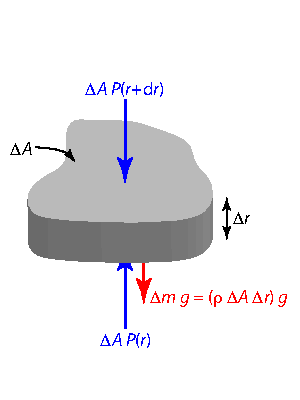
\includegraphics[width=\linewidth]{hydrostatic-equilibrium}
\caption[A fluid element in hydrostatic equilibrium]{A fluid element in hydrostatic equilibrium.
\label{f.hydrostatic-equilibrium}}
\end{marginfigure}

The force on the upper face is $\Delta A\times P(r+\Delta r)$; on the lower face, $\Delta A\times P(r)$.  Here $P(r)$ is the pressure.  For the element to be in hydrostatic equilibrium the forces must balance,
\[
        \Delta A \left[ -P(r+\Delta r) + P(r) - \Delta r \rho g(r)  \right] = 0;
\]
substituting for $g(r)$, dividing by $\Delta r$, taking the limit $\Delta r \to 0$ gives us the equation of hydrostatic equilibrium:
\begin{equation}\label{e.hydrostatic-equilibrium}
        \DD{P}{r} = -\rho \frac{Gm(r)}{r^{2}}.
\end{equation}
Here the mass enclosed within radius $r$ is
\begin{equation}\label{e.mass-continuity}
	m(r) = 4\pi \int_{0}^{r}\rho(r)r^{2}\,\dif r,
\end{equation}
with $\rho$ being the mass density. We can't solve these equations yet because we don't have a relation---yet---between $P$ and $\rho$.  But rather than wait to develop all of the physics we need, we are going to leapfrog ahead by \emph{assuming} a simple form for $\rho(r)$ and using that to understand better how stars work.

\begin{exercisebox}[A star of constant density]
\label{ex.constant-density-star}
Let's suppose that $\rho$ is constant throughout the star. 
In what follows, you should be able to express everything in terms of the star's mass $M$ and radius $R$, along with physical constants such as $G$ and $\kB$.

\begin{enumerate}
\item\label{rhoc} First, find $\rho$ in terms of the total mass $M$ and radius $R$.

\item Next, solve equation~(\ref{e.mass}) to find $m(r)$ in terms of $M$ and $r/R$.

\item\label{Pc} Use this expression for $m(r)$ and your expression for $\rho$ to integrate equation~(\ref{e.hydrostatic-equilibrium}) and to find the pressure at the center, $P_{c} = P(r=0)$.

\item
Now that we have an expression for the central pressure in terms of $M$ and $R$, let's try to understand what it means. For an ideal gas, the pressure, density, and temperature are related:
\begin{equation}\label{e.eos}
P = \rho\left(\frac{\kB}{\mu\mb}\right) T,
\end{equation}
where $\mb = 1/12\times(\textrm{mass of a \carbon\ atom})$ and $\mu$ is the mean molecular weight---the average mass of a particle in the gas.  We'll show how to compute $\mu$ later; for now, just treat it as a constant. Use your result from parts \ref{Pc} and \ref{rhoc}, as well as equation~(\ref{e.eos}) to find the central temperature of the star, in terms of $G$, $M$, $R$, and the mean molecular weight of the gas $\mu$.  Evaluate $T_{c}$ for $M=M_{\odot}$, $R=R_{\odot}$, and $\mu = 0.6$.  Do you get a reasonable result?
\end{enumerate}
\end{exercisebox}

\section{A closer look at hydrostatic equilibrium}
\label{s.closer-look}

Let's imagine what would happen if the star fell out of equilibrium.  Suppose we could turn off the pressure.  The star would collapse; how long would this take?  Let's calculate the amount of time a particle would need to free-fall from the surface to the center.  We can get this from Kepler's law. Start with a circular orbit and deform it while keeping the center at one focus, as shown in Fig.~\ref{f.fall-to-center}.  

The limit of these increasingly eccentric orbits is a fall into the center.  The time is one-half of an orbital period, and the semi-major axis in this limiting case is $a = R/2$:
\[
\tau_{\mathrm{ff}} = \frac{T}{2} = \frac{\pi}{\sqrt{GM}} \left(\frac{R}{2}\right)^{3/2}.
\]
Notice that we again have the combination $\sqrt{R^{3}/M}$.  Let's convert this into an expression involving the mean density $\bar{\rho}$:
\begin{equation}\label{e.tff}
\tau_{\mathrm{ff}} = \left(\frac{3}{32\pi}\right)^{1/2}\left(\frac{1}{G}\frac{4\pi R^{3}}{3M}\right)^{1/2} = \left(\frac{3}{32\pi}\right)^{1/2} \frac{1}{\sqrt{G\bar{\rho}}}.
\end{equation}
The time to collapse is proportional to $1/\sqrt{G\bar{\rho}}$ and depends on the average density of the star. We call $t_{\mathrm{dyn}} \equiv 1/\sqrt{G\bar{\rho}}$ the \emph{dynamical timescale} of the star.

\begin{marginfigure}
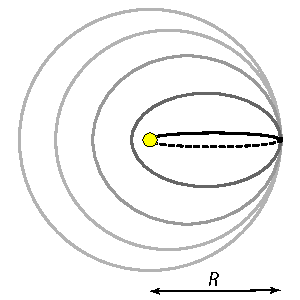
\includegraphics[width=\linewidth]{fall-to-center}
\caption[Fall to center]{\label{f.fall-to-center} Deformation of an orbit until it becomes a fall to the center, denoted by the yellow dot.}
\end{marginfigure}

Let's avoid a collapse by turning the pressure back on.  If part of the star is falling inward, the gas within the star will be compressed, the pressure will rise, and hydrostatic equilibrium will be restored.  How quickly can the star respond? A change is pressure is communicated to the rest of the star by sound waves, which travel at a speed (see Box~\ref{b.sound-speed})
\begin{equation}\label{e.speed-of-sound}
c_{s} = \left(\gamma\frac{P}{\rho}\right)^{1/2}
	= \left(\gamma\frac{\kB T}{\mu\mb}\right)^{1/2}.
\end{equation}
Here $\gamma$ is the adiabatic index: for an ideal monatomic gas, $\gamma = 5/3$.  How long would it take for a sound wave to go a distance $R$?  Using the expression for the average temperature of a constant density sphere from eq.~(\ref{e.mean-T-rho}), we find
\[
	\tau_{\mathrm{sc}} = \frac{R}{c_{s}} = R\left(\frac{3R}{GM}\right)^{1/2}
		= \left(\frac{3}{2\sqrt{\pi}}\right)\frac{1}{\sqrt{G\bar{\rho}}}.
\]
Both the sound-crossing time, $\tau_{\mathrm{sc}}$, and the free-fall time, $\tau_{\mathrm{ff}}$, are approximately equal to the dynamical timescale $1/\sqrt{G\bar{\rho}}$.  This is another way of looking at hydrostatic equilibrium: the star is able to remain in balance because the time for pressure disturbances to propagate, $\tau_{\mathrm{sc}}$, is comparable to the time for large-scale motions of the fluid, $\tau_{\mathrm{ff}}$.

\begin{sidebar}[The sound speed]
\label{b.sound-speed}
Suppose we have a long tube filled with gas at pressure $P(x,t) = P_{0}$, density $\rho(x,t) = \rho_{0}$, and velocity $u(x,t) = U_{0} = 0$. We then tap on one end of the tube; this causes a disturbance to propagate down the tube. Let's look at a small mass of fluid, located between $x$ and $x+\Delta x$; if the cross-sectional area of the tube is $A$, then the mass in this small volume is $\rho A\,\Delta x$.

As a result of the disturbance, the pressure in the tube becomes $P(x,t) = P_{0}+\sigma P_{1}(x,t)$. In this expression, $\sigma$ is a bookkeeping parameter that we'll eventually set to unity. We will expand our equations and keep only terms that are linear in $\sigma$. The fluid will also acquire a velocity $u(x,t) = \sigma u_{1}(x,t)$. This compresses or rarifies the gas: $\rho(x,t) = \rho_{0} + \sigma\rho_{1}(x,t)$.  Because the pressure in the tube is no longer uniform, our small mass will accelerate: 
\begin{eqnarray*}
	\rho A\,\Delta x \ddt{u} &=& A\,\Delta x\,(\rho_{0} + \sigma\rho_{1})\ddt{(0 + \sigma u_{1})}\\
	&\approx& \sigma\left[A\,\Delta x \rho_{0}\ddt{u_{1}}\right] + \mathcal{O}(\sigma^{2}).
\end{eqnarray*}
The corresponding force on our mass is
\[
	A \left[ P(x) - P(x+\Delta x) \right] \approx -\sigma A \left[P_{1}(x+\Delta x)-P_{1}(x)\right];
\]
equating this to the expression---to order $\sigma$---for the acceleration, taking the limit $\Delta x\to 0$, and canceling common factors gives
\begin{equation}\label{e.sound-speed-ut}
	\ddt{u_{1}} = -\frac{1}{\rho_{0}}\ddx{P_{1}}.
\end{equation}
Because of the non-uniform velocity, the volume and hence density of our little mass will also change:
\[
	\ddt{V} = A\left[u(x+\Delta x)-u(x)\right] 
		= \sigma A\,\Delta x\left[\frac{u_{1}(x+\Delta x)-u_{1}(x)}{\Delta x}\right]
\]
or
\begin{equation}\label{e.sound-speed-lnVt}
	\frac{1}{V}\ddt{V} = \sigma \ddx{u_{1}}.
\end{equation}
This change in volume is related to the change in pressure. We are interested in fluctuations that are sufficiently quick that no heat is transferred into or out of our mass. This is an adiabatic process, for which $PV^{\gamma} = \mathrm{const.}$. Here $\gamma$ is called the adiabatic index; for an ideal gas, this is the ratio of specific heats, $\gamma = C_{P}/C_{V}$.

As the pressure changes adiabatically from $P_{0}$ to $\sigma P_{1}$, the volume changes as
\[
	\frac{\dif V}{V} = \dif\ln V = -\frac{1}{\gamma}\dif\ln P.
\]
Hence
\begin{equation}\label{e.sound-speed-lnVt-2}
	\ddt{\ln V} = -\frac{1}{\gamma}\ddt{\ln (P_{0} + \sigma P_{1})} \approx 
		-\frac{\sigma}{\gamma P_{0}}\ddt{\ln P_{1}} = \sigma \ddx{u_{1}}.
\end{equation}
The last equality comes from equation (\ref{e.sound-speed-lnVt}).

We therefore have two equations for the perturbed velocity to order $\sigma$:
\begin{eqnarray*}
\ddt{u_{1}} &=& -\frac{1}{\rho_{0}} \ddx{P_{1}}\\
\ddx{u_{1}} &=& -\frac{1}{\gamma P_{0}} \ddt{P_{1}};
\end{eqnarray*}
differentiating the top equation with respect to $x$ and the bottom with respect to $t$, and equating the expressions for $\partial^{2}u_{1}/\partial t\partial x$ gives
\begin{equation}\label{e.sound-speed}
\frac{\partial^{2} P_{1}}{\partial t^{2}} = \left(\frac{\gamma P_{0}}{\rho_{0}}\right)
	\frac{\partial^{2} P_{1}}{\partial x^{2}}.
\end{equation}
This is the equation for a wave: the solutions are $P_{1}(x,t) = P_{1}(x\pm c_{s}t)$, where the sound speed is $c_{s} = \sqrt{\gamma P/\rho}$.
\end{sidebar}

For the sun, $\bar{\rho} = \val{1400}{\kilo\gram\usk\meter^{-3}} = \val{1.4}{\grampercc}$; this is just a bit denser than you.  The dynamical timescale for the sun is about one hour.

\begin{exercisebox}[Sound-crossing time]
The central temperature $T_{c}$ is a measure of the average kinetic energy of a particle at the stellar center. Use the central temperature that you found for the constant density star in exercise~\ref{ex.constant-density-star} and estimate the time that such a particle would take to cross a distance $R$. How does this time compare to the orbital period of a satellite orbiting just outside the stellar surface?
\end{exercisebox}

\section{Virial Equilibrium}
\label{s.virial-equilibrium}

With the assumption that $\rho = \textrm{constant}$, we showed (exercise~\ref{ex.constant-density-star}) that the central temperature and pressure depended on the total mass $M$, total radius $R$, and the gravitational constant $G$ as
\begin{eqnarray}
\label{e.Tc}
T_{c} &=& \frac{1}{2}\left\{\frac{GM}{R}\frac{\mu\mb}{\kB}\right\}\\
\label{e.Pc}
P_{c} &=& \frac{3}{8\pi}\left\{\frac{GM^{2}}{R^{4}}\right\}.
\end{eqnarray}
Here $\mu\mb$ is the average mass of a particle in the plasma\sidenote{%
The constant $\mb$ is defined as $1/12$ the mass of a \carbon\ atom.}.
Our task now is to show that the scalings of $T_{c}$ and $P_{c}$ with $M$ and $R$---the quantities in $\{\,\}$---hold in general for an a star in mechanical equilibrium.

To show this, we are going to employ a form of the \emph{virial theorem}.  Suppose we have a collection of $N$ particles, all moving about and exerting forces on one another.  If we let this system settle down into some kind of bound configuration, then we can add up the kinetic and potential energies of all the particles to get a total kinetic energy $K$ and a total potential energy $\Omega$. The virial theorem asserts that $K$ is proportional to, and comparable in magnitude to, $\Omega$; indeed if the potential between a pair of particles scales as $r^{-1}$, $r$ being the distance between the particles, then $K = -\Omega/2$, as we'll now show.

Let us take the position and momentum of particle $i$ to be $\bvec{r}_{i} = (x_{i},y_{i},z_{i})$ and $\bvec{p}_{i}=(p_{x},p_{y},p_{z})$.  Then the total kinetic energy is
\begin{eqnarray}
\nonumber
	K &=& \frac{1}{2}\sum_{i=1}^{N}\bvec{p}_{i}\vdot\DDt{\bvec{r}_{i}}\\
		&=& \frac{1}{2}\left[\DDt{}\left(\sum_{i=1}^{N}\bvec{p}_{i}\vdot\bvec{r}_{i}\right) - \sum_{i=1}^{N}\bvec{r}_{i}\vdot\DDt{\bvec{p}_{i}}\right].
\label{e.expand-K}
\end{eqnarray}
The quantity $G = \sum_{i}\bvec{p}_{i}\vdot\bvec{r}_{i}$ is called the ``virial'' of the system.  By expressing the force $\bvec{F}_{i} = \dif\bvec{p}_{i}/\dif t$ on particle $i$ as the gradient of a potential $\Omega$, $\bvec{F}_{i} = -\grad_{i}\Omega$, we can rewrite eq.~(\ref{e.expand-K}) as
\begin{equation}\label{e.virial-deriv-1}
	2K = \DDt{G} + \sum_{i=1}^{N}\bvec{r}_{i}\vdot\grad_{i}\Omega.
\end{equation}
So far, we just shuffled and relabeled terms.  The crucial step comes in taking the time-average of the kinetic energy, which we'll denote by $\langle\;\rangle$:
\[	\langle f\,\rangle \equiv \lim_{\tau\to\infty} \frac{1}{\tau}\int_{0}^{\tau}f(t)\,\dif t. \]
Applying this to equation~(\ref{e.virial-deriv-1}) gives
\begin{eqnarray*}
	2\langle K\,\rangle &=&
		 \left\langle\DDt{G}\right\rangle 
		+ \left\langle\sum_{i=1}^{N}\bvec{r}_{i}\vdot\grad_{i}\Omega\right\rangle\\
	&=& \lim_{\tau\to\infty}\left[\int_{0}^{\tau}\,\DDt{G}\,\dif t\right] 
		+ \left\langle\sum_{i=1}^{N}\bvec{r}_{i}\vdot\grad_{i}\Omega\right\rangle\\
	&=& \underbrace{\lim_{\tau\to\infty}\left[\frac{G(\tau)-G(0)}{\tau}\right]}_{\mathrm{I}}
		+ \underbrace{\left\langle\sum_{i=1}^{N}\bvec{r}_{i}\vdot\grad_{i}\Omega\right\rangle}_{\mathrm{II}}
\end{eqnarray*}
Now, if the system is bound and in mechanical equilibrium, then the positions and momenta of all particles are finite: none of the particles can escape, and the system doesn't violently collapse so that momenta are diverging.  Hence both $G(\tau)$ and $G(0)$ are finite numbers, so as $\tau\to\infty$, term I vanishes.

As for term II, we can show that if the potential between pairs of particles depends on $1/r$, where $r$ is the distance between those particles, then term II is just $-\Omega$ (see Box~\ref{b.working-vectors}).  For now, I'll give a rough argument of why this is so:  in a spherically symmetric system, then the potential just depends on the distance $r$ from the origin; and since
\[
	r\dd{}{r} \left(\frac{1}{r}\right) = -\frac{1}{r},
\]
the last term is just $-\Omega$ and our equation is
\begin{equation}\label{e.virial-theorem}
2\langle K\,\rangle + \langle \Omega\rangle = 0.
\end{equation}
This is the virial theorem.

\begin{sidebar}[Working with vectors]
\label{b.working-vectors}
In this sidebar we'll show that the second term in equation~(\ref{e.virial-deriv-1}) is
\begin{equation}\label{e.term-2}
	\sum_{i=1}^{N}\bvec{r}_{i}\vdot\grad_{i}\Omega = -\Omega.
\end{equation}
First, we need an expression for $\Omega$. Suppose we pick a pair of particles, $i$ and $k$.  The potential between this pair is
\[
	-\frac{Gm_{i}m_{k}}{r_{ik}} = -\frac{Gm_{i}m_{k}}{\sqrt{(\bvec{r}_{i}-\bvec{r}_{k})^{2}}}.
\]
Our total potential consists of a sum over the potentials between all $N(N-1)/2$ unique pairs of particles,
\[
	\Omega = -\frac{Gm_{1}m_{2}}{\sqrt{(\bvec{r}_{1}-\bvec{r}_{2})^{2}}} - \ldots 
	-\frac{Gm_{i}m_{k}}{\sqrt{(\bvec{r}_{i}-\bvec{r}_{k})^{2}}} - \dots
\]
When we take the derivative in eq.~(\ref{e.term-2}), we apply $\bvec{r}_{i}\vdot\grad_{i}$ to each term in the potential.  For the term with the pair $i$, $k$, this will give
\begin{eqnarray*}
	\lefteqn{\sum_{i=1}^{N}\bvec{r}_{i}\vdot\grad_{i}\left(-\frac{Gm_{i}m_{k}}{\sqrt{(\bvec{r}_{i}-\bvec{r}_{k})^{2}}}\right)} \\
	&=& -Gm_{i}m_{k}\left[\bvec{r}_{i}\vdot\grad_{i}\left(\frac{1}{\sqrt{(\bvec{r}_{i}-\bvec{r}_{k})^{2}}}\right) + \bvec{r}_{k}\vdot\grad_{k}\left(\frac{1}{\sqrt{(\bvec{r}_{i}-\bvec{r}_{k})^{2}}}\right)\right].
\end{eqnarray*}
Since many of you aren't yet comfortable with vector expressions, we'll do this in detail for the $x$-component:
\begin{eqnarray*}
	\lefteqn{\left[\bvec{r}_{i}\vdot\grad_{i}\left(\frac{1}{\sqrt{(\bvec{r}_{i}-\bvec{r}_{k})^{2}}}\right) + \bvec{r}_{k}\vdot\grad_{k}\left(\frac{1}{\sqrt{(\bvec{r}_{i}-\bvec{r}_{k})^{2}}}\right)\right]_{x}}\\
	&=& x_{i}\dd{}{x_{i}}\left(\frac{1}{\sqrt{(\bvec{r}_{i}-\bvec{r}_{k})^{2}}}\right)
		+ x_{k}\dd{}{x_{k}}\left(\frac{1}{\sqrt{(\bvec{r}_{i}-\bvec{r}_{k})^{2}}}\right) \\
		&=& -\frac{x_{i}(x_{i}-x_{k})}{(\bvec{r}_{i}-\bvec{r}_{k})^{3/2}}
		+ \frac{x_{k}(x_{i}-x_{k})}{(\bvec{r}_{i}-\bvec{r}_{k})^{3/2}}\\
		&=& -\frac{(x_{i}-x_{k})^{2}}{(\bvec{r}_{i}-\bvec{r}_{k})^{3/2}}
\end{eqnarray*}
The $y$- and $z$-components are similar, giving
\begin{eqnarray*}
	\sum_{i=1}^{N}\bvec{r}_{i}\vdot\grad_{i}\left(-\frac{Gm_{i}m_{k}}{\sqrt{(\bvec{r}_{i}-\bvec{r}_{k})^{2}}}\right) &=& Gm_{i}m_{k}
	\frac{(\bvec{r}_{i}-\bvec{r}_{k})^{2}}{(\bvec{r}_{i}-\bvec{r}_{k})^{3/2}}\\
 &=& -\left(-\frac{Gm_{i}m_{k}}{\sqrt{(\bvec{r}_{i}-\bvec{r}_{k})^{2}}}\right).
\end{eqnarray*}
This can be done for every term in the sum, with the final result that
\[
	\sum_{i=1}^{N}\bvec{r}_{i}\vdot\grad_{i}\Omega = -\Omega.
\]
\end{sidebar}

For an ideal monatomic gas in thermal equilibrium, the mean kinetic energy of a particle in the gas is $K = (3/2)\kB T$, and we therefore may define an average temperature
\begin{equation}\label{e.Tbar}
	2 K = 3 N\kB \bar{T} = -\Omega.
\end{equation}
The total number of particles is $N=M/(\mu\mb)$, and so
\begin{equation}\label{e.mean-T}
\bar{T} = -\frac{1}{3}\Omega\frac{\mu\mb}{M\kB}.
\end{equation}
The total potential of the system depends on only three parameters: $G$, $M$, and $R$.  The only way to make a quantity having dimensions of energy is for
\[ \Omega \propto -\frac{GM^{2}}{R}, \]
and so
\[ \bar{T} \propto \frac{GM}{R}\frac{\mu\mb}{\kB}.  \]
By using the ideal gas law, $\bar{P} = \bar{\rho}(\kB/\mu\mb)\bar{T}$, we find
\[ \bar{P} \propto \frac{GM^{2}}{R^{4}}. \]
As a concrete example, let's compute $\Omega$ for a constant density sphere.
If we bring a small amount of mass $\dif m$ from infinity onto a sphere of mass $m$ and radius $r$, then the change in potential is \[ \dif\Omega = -\frac{Gm}{r}\,\dif m. \]
For a constant density, $r = R(m/M)^{1/3}$; upon substituting for $r$ we have
\[
	\Omega_{\textrm{const.\ den.}} = - \int_{0}^{M}\frac{GM^{1/3} m^{2/3}}{R}\,\dif m = -\frac{3}{5}\frac{GM^{2}}{R}.
\]
Using this in equation~(\ref{e.mean-T}) gives us the mean temperature, and hence pressure, for a constant density sphere,
\begin{eqnarray}\label{e.mean-T-rho}
\bar{T} &=& \frac{1}{5}\frac{GM}{R}\frac{\mu\mb}{\kB},\\
\label{e.mean-P}
\bar{P} &=& \frac{3}{20\pi}\frac{GM^{2}}{R^{4}}.
\end{eqnarray}
These are comparable to the central values, eqn.~(\ref{e.Tc}) and (\ref{e.Pc}).

\begin{table}
\caption{\label{t.stellar-properties} Masses, radii, and luminosities for selected stellar types.}
\begin{tabular}{ld{4.2}d{3.2}d{1.2}d{1.2}d{1.2}d{2.3}}
 & \tabhead{B2} & \tabhead{B8} & \tabhead{F0} & \tabhead{G5} & \tabhead{M0} & \tabhead{M7}\\ 
\hline
$M/\Msun$ & 9.8 & 3.8 & 1.6 & 0.92 & 0.51 & 0.12\\
$R/\Rsun$ & 5.6 & 3.0 & 1.5 & 0.92 & 0.60 & 0.18\\
$L/\Lsun$ & 5800.0    & 180.0 & 6.5 & 0.79 & 0.08 & 0.003\\
%$\rho_{c}/\rho_{c,\odot}$ & 0.06 & 0.14 & 0.47 & 1.18 & 2.36 & 20.58\\
%\rowcolor{yellow}
%$T_{c}/T_{c,\odot}$ & 1.75 & 1.27 & 1.07 & 1.00 & 0.85 & 0.67\\
%$P_{c}/P_{c,\odot}$ & 0.10 & 0.18 & 0.51 & 1.18 & 2.01 & 13.72\\
\end{tabular}
\end{table}

\begin{exercisebox}\label{ex.stellar-properties}
We can infer a great deal from our simple virial scalings. Table~\ref{t.stellar-properties} provides masses, radii, and luminosities, in units of $\Msun$, $\Rsun$, and $\Lsun$, for stars from type B to type M.  
Using the constant density model, compute $\rho/\rho_{\odot}$, $T_{c}/T_{c,\odot}$, and $P_{c}/P_{c,\odot}$. You should find that each quantity depends only on $m=M/\Msun$ and $r=R/\Rsun$. Describe your findings: do $P_{c}/P_{c,\odot}$, $\rho/\rho_{\odot}$, and $T_{c}/T_{c,\odot}$ vary in a similar fashion? If not, how do they change with stellar type?
\end{exercisebox}

%Notice that $P_{c}$ and $\rho_{c}$ are larger for lower-mass stars. An even more surprising finding from this table is how little $T_{c}$ varies. This table spans nearly two decades in mass and six decades in luminosity, and yet $T_{c}$ varies by only a factor of three.  As we'll derive later, this is a consequence of the fusion reactions being extremely sensitive to temperature.

\section{Contraction to the main sequence}
\label{s.stellar-contraction}

Stars are born when a cold, dense\sidenote{Dense is a relative term; here we mean $\sim 100$ \emph{atoms} per cubic centimeter} cloud of gas and dust becomes unstable to gravitational collapse. The details of this process is a topic of current research; for our purposes, however, after a period of time a pre-main sequence star forms.  This object is in hydrostatic balance, but with a radius much larger than its main-sequence value.  As you know from the previous discussion, its central temperature will therefore be too low for fusion reactions to be important.  What happens to this object?

The pre-main sequence star is in hydrostatic balance, so it doesn't collapse. But the interior, and hence the surface, is warm, so it radiates energy.  The only source of energy is gravitational, so the pre-main sequence star \emph{must} contract.  How long would this take?  For our sun, the total energy is
\[
	E_{\odot} = K + \Omega = \Omega/2 \approx -\frac{G\Msun^{2}}{\Rsun};
\]
the time to radiate this energy away is
\begin{equation}\label{e.kelvin-helmholtz}
t_{\mathrm{KH}} = \frac{|E_{\odot}|}{\Lsun} \approx \frac{G\Msun^{2}}{\Rsun\Lsun} \approx \val{\sci{3}{7}}{\yr}.
\end{equation}
This timescale is called the \emph{Kelvin-Helmholtz timescale}.  Since $t_{\mathrm{KM}} \gg t_{\mathrm{dyn}}$ the star is, to an excellent approximation, in hydrostatic equilibrium throughout the whole contraction.
%
%As the star contracts and $R$ decreases, the central density, pressure, and temperature increase.  When the central temperature becomes sufficiently hot, the heating from nuclear reactions rapidly increases and supplies enough energy to offset that radiated from the surface.  At this point the star is on the main-sequence, where it remains until the hydrogen fuel is exhausted from its core.

\begin{exercisebox}
Using the constant-density model (note that constant here means ``constant throughout the star at any given time'' and the virial relations, give a qualitative sketch for how the pressure, density, temperature, radius, and total energy change with time as the protostar contracts.
\end{exercisebox}


\chapter{Shining Star}\label{ch.radiative-transport}
% !TEX root = ../intro-stellar-physics.tex

We saw in chapter~\ref{ch.basic-stellar-properties} that the equilibrium central temperature of a self-gravitating object---such as a star---with an ideal gas EOS depends \emph{solely} on the mass, radius, and composition of that star. For the Sun, this temperature is $\approx \val{15}{\Mega\K}$ and much higher than the surface effective temperature $T_{\!\mathrm{eff,\odot}} = \val{5780}{\K}$. The photons emitted from the Sun are coming from the cooler surface layers.

\newthought{Photons in a plasma, such as in the interior of the sun, transport energy.}  Were the sun transparent, these photons would immediately stream out, and the sun would release its stored energy in a fiery blast.  This doesn't happen: a photon can only travel a short distance before being scattered or absorbed. The net effect is that radiation generated in the core must travel a tortuous path, rather like a pinball, before reaching the surface and escaping.

\section{Interaction of radiation and matter}\label{s.interaction-radiation-matter}

How far does a photon---or any particle, for that matter---travel, on average, in the interior of the sun? Imagine a particle traveling with speed $v$.  Draw a cylinder, of length $\ell$ and cross-sectional area $\mathcal{A}$, around its path, as shown in Fig.~\ref{f.MFP}. What the particle ``sees'' is that the cylinder is partly blocked by obstacles---other particles in its path.
\begin{marginfigure}
    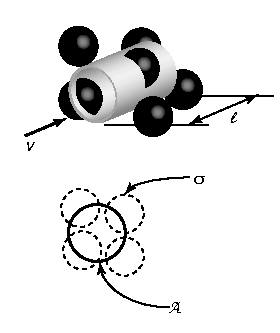
\includegraphics[width=\linewidth]{mean-free-path}
    \caption{\label{f.MFP} Schematic of a particle incident on a group of scattering or absorbing particles.}
\end{marginfigure}

\newthought{What is the probability of our particle making it through the cylinder unscathed?} The probability of the particle hitting an obstacle is the ratio
\[
    \mathcal{P} = \frac{\textrm{total area covered by obstacles}}{\textrm{area of cylinder}}
\]
Denote the cross-sectional area of the other particles by $\sigma$. If the density of obstacles is $n$, then the number of obstacles in the cylinder is $n\times(\mathcal{A}\ell)$, and therefore the fraction of the area blocked by the obstacles is
\begin{equation}
    \mathcal{P} = \frac{n\times(\mathcal{A}\ell)\times\sigma}{\mathcal{A}} = n\sigma\ell.
\label{e.prob-MFP}
\end{equation}
\marginnote{We are taking $\ell$ and $\mathcal{A}$ sufficiently small that we don't have to worry about particles overlapping.}
The particle will suffer a collision when $\mathcal{P}\to 1$, or when
\begin{equation}\label{e.MFP}
    \ell = \frac{1}{n\sigma}.
\end{equation}
We call $\ell$ the ``mean free path''.

\begin{marginfigure}[3\baselineskip]
    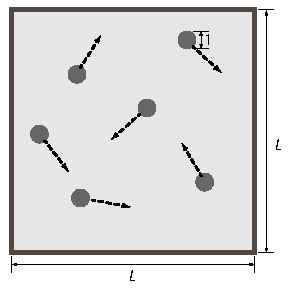
\includegraphics[width=\linewidth]{air-hockey-mfp}
    \caption[Mean free path of a hockey puck]{\label{f.MFP-2D}Schematic for Exercise~\ref{ex.MFP-2D}}
\end{marginfigure}
\begin{exercisebox}[Mean free path of a hockey puck]\label{ex.MFP-2D}
    Suppose we have a flat, slippery surface on which hockey pucks are sliding around, as shown in Fig.~\ref{f.MFP-2D}. The pucks bounce off the walls as they slide around.  Suppose there are $N$ pucks, each with unit diameter, and the table is square with sides of length $L$.  Estimate the mean free path of a puck.
\end{exercisebox}

Although we have motivated this derivation with a classical picture, the cross-section $\sigma$ is just related to the probability of an interaction and can therefore be defined for quantum mechanical systems.

\begin{exercisebox}[Mean free path for electron scattering]\label{ex.MFP}
    In the sun, free electrons scatter photons; the cross-section for this is
    \[
    \sigma_{\mathrm{Th}} = \left(\frac{8\pi}{3}\right)\left(\frac{e^2}{m_e c^2}\right)^2 = \val{\sci{6.65}{-27}}{\meter^2}.
    \]
    What is the mean free path against this process for a photon at the average density of the solar interior?
\end{exercisebox}

As the ray of light traverses a small distance $\Delta s$ through some matter, the probability of a photon being absorbed is $\mathcal{P} = n\sigma\Delta s$. Thus, out of every $N$ photons, $\Delta N = N \times\mathcal{P} = N\times n\sigma\Delta s$ are absorbed. Since the intensity $I_{\nu}$ is proportional to the number of photons, the change in intensity is just
\[ \Delta I_{\nu} = -n\sigma I_{\nu}\Delta s. \]
Taking the limit $\Delta s\to0$, we obtain an equation for the absorption of light,
\begin{equation}\label{e.absorption-microscopic}
\left.\DD{I_{\nu}}{s}\right|_{\mathrm{absorption}} = -n\sigma I_{\nu}.
\end{equation}
Rather than work with the microscopic cross-section, it is convenient to define the \newterm{absorption opacity},
\[
	\kapabs = \frac{n\sigma}{\rho},
\]
so that $\dif I_{\nu}/\dif s = -\rho\kapabs I_{\nu}$. The units of opacity are $\cm^{2}/\gram$. We use a subscript $\nu$ to indicate that the opacity is a function of frequency. In terms of the opacity, the photon mean free path is $\ell = (\rho\kapabs)^{-1}$.

\begin{exercisebox}[Attenuation of light in an absorbing medium]
A ray of light crosses a slab of absorbent material. Calculate the intensity $I_{\nu}$ as a function of distance traveled. Your expression should be in terms of $\rho$ and $\kapabs$. How far does the ray go before its intensity has dropped to $1/e$ of its original value?
\end{exercisebox}

\newthought{In addition to absorbing photons, the matter can also spontaneously emit them.} Denote the power emitted per wavelength per volume per angle by $\rho j_{\nu}$. After traveling a distance $\Delta s$ through matter with this \newterm{emissivity}, the ray will increase in intensity by $\rho j_{\nu}\Delta s$; or
\begin{equation}\label{e.emission-microscopic}
\left.\DD{I_{\nu}}{s}\right|_{\mathrm{emission}} = \rho j_{\nu}.
\end{equation}

\begin{exercisebox}[Combined absorption and emission]
Suppose a ray traverses matter that both absorbs (opacity $\kapabs$) and emits (emissivity $j_{\nu}$), so that
\[	\DD{I_{\nu}}{s} = \rho j_{\nu} - \rho\kapabs I_{\nu}. \]
Solve for $I_{\nu}(s)$, and show that as $s\to\infty$, $I_{\nu}\to j_{\nu}/\kapabs$.
\label{ex.intensity-at-large-depth}
\end{exercisebox}

\newthought{Finally, the matter can also scatter light.} This removes photons from a ray, similar to absorption, but it also adds them into a ray propagating in a different direction. 
If we assume that the direction into which the photon is scattered is random and isotropic (as is most often the case), then if the intensity in our ray is greater than the angle-average $J_{\nu}$, scattering will cause a net reduction in intensity as more photons are scattered out of the ray than are scattered into it. Conversely, if $I_{\nu} < J_{\nu}$, then more photons will be scattered into the ray than out of it. Thus, the effect of scattering can be described via
\begin{equation}\label{e.scattering-microscopic}
\left.\DD{I_{\nu}}{s}\right|_{\mathrm{scattering}} = -\rho\kapscat \left(I_{\nu} - J_{\nu}\right).
\end{equation}

\section{The equation of radiative transfer}
\label{s.equation-radiative-transfer}

Combining our expressions for absorption, emission, and scattering gives us the full expression for how the intensity changes along a ray,
\begin{equation}\label{e.transfer-equation}
\DD{I_{\nu}}{s} = -\rho\left(\kapabs + \kapscat\right) I_{\nu} + \rho j_{\nu} + \rho\kapscat J_{\nu}.
\end{equation}
This is a complicated \newterm{integrodifferential} equation: it contains both the derivative $\dif I_{\nu}/\dif s$ of the intensity as well as its integral $J_{\nu} = (4\pi)^{-1}\int I_{\nu}\,\dif\Omega$.

In general, eq.~(\ref{e.transfer-equation}) must be solved numerically; but conditions in the deep interior of the star and near the surface allow us to make simplifying approximations and to obtain a solution that gives some insight into the physics. First, let's clean up the equation: divide through by $\rho\kappa_{\nu}\equiv\rho(\kapabs + \kapscat)$,
\[
	\frac{1}{\rho\kappa_{\nu}}\dd{I_{\nu}}{s} = -I_{\nu} + \left[\frac{j_{\nu} + \kapscat J_{\nu}}{\kappa_{\nu}}\right].
\]
Next, define a new quantity, the \newterm{optical depth} $\tau_{\nu}$ via the equation
\[
	\dd{\tau_{\nu}}{s} = \rho\kappa_{\nu} = \rho(\kapabs+\kapscat),
\]
which allows us to change variables, $\dif I_{\nu}/\dif s = (\dif I_{\nu}/\dif\tau_{\nu})\cdot(\dif\tau_{\nu}/\dif s)$; and finally define the \newterm{source function} $S_{\nu}$ as the term in $\left[\cdot\right]$. Doing all that gives us the simpler-looking equation,
\[
	\DD{I_{\nu}}{\tau_{\nu}} = -I_{\nu} + S_{\nu}.
\]
This prettifying doesn't advance us any closer to the solution, but notice! The optical depth has a simple meaning:
\[
	\tau_{\nu} = \int_{0}^{s} \rho\kappa_{\nu}\,\dif s = \int_{0}^{s} n\sigma_{\nu}\,\dif s = \int_{0}^{s} \frac{\dif s}{\lambda}.
\]
That is, the optical depth measures distance along the ray in units of mean free path. Said differently, if you have traveled one optical depth, then you have gone one mean free path. We also see from this equation that $I_{\nu}\to S_{\nu}$ as $\tau_{\nu}\to\infty$ (cf.\ exercise~\ref{ex.intensity-at-large-depth}).

Thus, if your object has $\tau_{\nu}\ll 1$, then photons are hardly affected by the medium and the object is nearly transparent; if, on the other hand, $\tau_{\nu} \gg 1$, then photons cannot go through the object: it is opaque, and the emission is determined by the emissivity (via the source function $S_{\nu}$) of the matter.

\begin{exercisebox}[Optical depth of the solar center]
For the electron scattering cross-section (Exercise~\ref{ex.MFP}), estimate the optical depth between the solar center and the solar photosphere.
\end{exercisebox}

\newthought{Suppose we are in a cavity in which the radiation and matter are in a steady-state}. 
The matter is not gaining or losing energy to the radiation. This requires balancing
\[ \left(\textrm{energy emitted per unit volume}\right) = \rho\int j_{\nu}\,\dif\nu\,\dif\Omega\] 
with
\[ \left(\textrm{energy absorbed per unit volume}\right) = \rho\int \kapabs I_{\nu}\,\dif\nu\,\dif\Omega,\]
so that
\begin{equation}\label{e.rad-equil}
\int_{0}^{\infty}\! \left(j_{\nu} - \kapabs J_{\nu}\right)\,\dif\nu = 0.
\end{equation}
We don't include scattering in this expression because scattering doesn't transfer energy between the radiation and the gas.

If, in addition, the matter and radiation are in thermal equilibrium, so that $J_{\nu} = B_{\nu}$, then eq.~(\ref{e.rad-equil}) implies that
\begin{equation}\label{e.detailed-balance}
\frac{j_{\nu}}{\kapabs} = B_{\nu}(T).
\end{equation}
Now $j_{\nu}$ and $\kapabs$ are properties of the matter, and do not depend on the state of the radiation field. Hence, equation~(\ref{e.detailed-balance}) must hold whenever the matter is in equilibrium, \emph{regardless of the state of the radiation field}.

\section{Radiative diffusion}

We can now examine how heat transport works in the deep interior of a star. First, we need to adjust our coordinates. In equation~(\ref{e.transfer-equation}), the coordinate $s$ is distance along a ray; but we are considering many different rays. We shall therefore use radial distance $r$ as a coordinate, and measure the optical depth it: $\dif\tau_{\nu} = \rho\kappa_{\nu}\,\dif r$. 
Since $\dif r = \mu\,\dif s$, where $\mu=\cos\theta$ is the cosine between $\dif s$ and $\dif r$ (Fig.~\ref{f.dr-ds-relation}), the equation of transfer becomes
\begin{equation}
\mu\DD{I_{\nu}}{r} = -\rho\kappa_{\nu}\left(I_{\nu} - S_{\nu}\right).
\end{equation}
\begin{marginfigure}
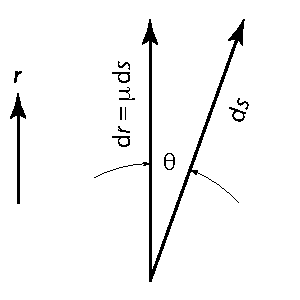
\includegraphics[width=\linewidth]{dr-ds-relation}
\caption{\label{f.dr-ds-relation} Schematic of coordinate for solving the radiative transport equation.}
\end{marginfigure}

\newthought{Let's examine the typical scales of terms in the radiative transfer equation, for conditions in the deep solar interior.} We'll start with eq.~(\ref{e.transfer-equation}), and indicate some expected scales:
\[
\underbrace{\mu\DD{I_{\nu}}{r}}_{\sim I_{\nu}/\Rsun} = -\underbrace{\rho\kappa_{\nu} I_{\nu}}_{\sim I_{\nu}/\lambda}  +\rho\kappa_{\nu} S_{\nu}.
\]
If we are far from the surface of the star, then we should expect the intensity to change over lengthscales comparable to $\Rsun$. Of course, it won't be exactly this, but---as we'll show---the exact value doesn't matter so long as $|\dif I_{\nu}/\dif s|$ is in the ballpark of $I_{\nu}/\Rsun$. Notice the enormous disparity in scales:
\[
	\frac{|\dif I_{\nu}/\dif r|}{\rho\kappa_{\nu}I_{\nu}} \sim \frac{\lambda}{\Rsun};
\]
the left-hand side is smaller than the terms on the right by the ratio of the mean free path to the solar radius. This implies that conditions are nearly homogeneous. They are also isotropic, so that $I_{\nu} = J_{\nu}$. We expect that collisions are fast enough so that the matter is in thermal equilibrium and $j_{\nu} = \kapabs B_{\nu}$. We also know from exercise~\ref{ex.intensity-at-large-depth} that $I_{\nu} \to j_{\nu}/\kapabs = B_{\nu}$.

We can't have $I_{\nu} = B_{\nu}$ exactly, however, since in that case there is no net flux! We'll treat the intensity as a perturbation to its thermal value:
\[ I_{\nu} = B_{\nu} + I_{\nu}^{(1)}, \]
where the superscript ``(1)'' indicates that this is a small correction. Inserting this expansion into eq.~(\ref{e.transfer-equation}) and keeping only the lowest-order terms on each side gives
\begin{equation}\label{e.perturbation-radiative-transfer}
I_{\nu}^{(1)} = -\mu\DD{B_{\nu}}{\tau_{\nu}}.
\end{equation}
$B_{\nu}$ depends on the temperature $T$, so $\dif B_{\nu}/\dif\tau_{\nu} = \dif B_{\nu}/\dif T \cdot \dif T/\dif \tau_{\nu}$. To get the flux, multiply eq.~(\ref{e.perturbation-radiative-transfer}) by $\mu$ and integrate over angles:
\[ F_{\nu} = \int\mu I_{\nu}^{(1)}\,\dif\Omega = -\int \mu^{2}\DD{B_{\nu}}{T}\,\DD{T}{\tau_{\nu}}\,\dif \Omega = -\frac{4\pi}{3} \DD{B_{\nu}}{T}\,\DD{T}{\tau_{\nu}}. \]
We can switch back to the radial coordinate:
\begin{equation}\label{e.specific-radiative-transport}
	F_{\nu} = -\frac{4\pi}{3}\left[\frac{1}{\rho\kappa_{\nu}}\dd{B_{\nu}}{T}\right]\DD{T}{r}.
\end{equation}
The term in $\left[\cdot\right]$ controls which frequencies are most responsible for energy transport.

\begin{exercisebox}[Transport by frequency]
\label{ex.radiative-transfer}
Let's examine the term $\left[\cdot\right]$ in eq.~(\ref{e.specific-radiative-transport}) more closely. Fig.~\ref{f.planck} shows $B_{\nu}$ and $\dif B_{\nu}/\dif T$ (top panel) and a hypothetical $\kappa_{\nu}$ (middle). Sketch $F_{\nu}$ on the bottom panel.  For which frequencies is it maximum?
\end{exercisebox}

\begin{marginfigure}
\includegraphics[width=\linewidth]{radiative-transfer-exercise}
\caption{\label{f.planck} Comparison of the Planck function and its derivative w.r.t.\ temperature, the opacity, and the specific flux.}
\end{marginfigure}

To get the total flux, we integrate $F_{\nu}$ over all frequencies. 
\begin{eqnarray*}
	F = \int_{0}^{\infty}F_{\nu}\,\dif\nu &=& -\frac{4\pi}{3} \left[\int_{0}^{\infty} \frac{1}{\rho\kappa_{\nu}}\dd{B_{\nu}}{T}\right]\DD{T}{r}\\
	&\equiv& -\frac{4\pi}{3}\frac{1}{\rho\kappa_{\mathrm{R}}}\dd{}{T}\left[\int_{0}^{\infty}B_{\nu}\,\dif\nu\right]\DD{T}{r}.
\end{eqnarray*}
Here we've defined the \newterm{Rosseland mean} of the opacity:
\begin{equation}\label{e.rosseland-opacity}
	\frac{1}{\kappa_{\mathrm{R}}} = \left(\int_{0}^{\infty} \dd{B_{\nu}}{T}\,\dif\nu\right)^{-1}\int_{0}^{\infty} \frac{1}{\kappa_{\nu}}\dd{B_{\nu}}{T}\,\dif\nu.
\end{equation}
This is done to put the equation in more familiar terms. Since (cf.\ eq.~[\ref{e.bolometric-thermal-flux}]) $\int B_{\nu}\,\dif\nu = \sigmaSB T^{4}/\pi = c a T^{4}/4\pi$, we can write the equation for the flux as
\begin{equation}
	F = -\frac{1}{3}\frac{c}{\rho\kappa_{\mathrm{R}}}\DD{}{r}aT^{4}.
\label{e.radiative-transfer}
\end{equation}
Equation (\ref{e.radiative-transfer}) is known as the equation for radiative diffusion, for reasons that will become apparent in the next section.

If we multiply the flux by the surface area of a shell in the star we obtain the luminosity $L = 4\pi r^{2} F$; we can therefore recast eq.~(\ref{e.radiative-transfer}) into an equation for the thermal gradient:
\begin{equation}
    \label{e.gradient-temperature}
    \DD{T}{r} = -\frac{3\rho\kappa_{R}}{4acT^3}\frac{L(r)}{4\pi r^2}.
\end{equation}

\begin{exercisebox}[Radiative transfer equation]
\label{ex.radiative-transfer-diffusion}
Let's dissect eq.~(\ref{e.radiative-transfer}) to see how it sets the luminosity.  
\begin{enumerate}
\item\label{p.F-L}
To keep the algebra simple, assume that $F$ is constant throughout the star and that $aT^{4}$ is linear in $r$---that is, $aT^{4} = aT_{c}^{4}(1-r/R)$.  Since $F$ is constant, you can express it in terms of the luminosity at the surface $L$.  Use this to transform eq.~(\ref{e.radiative-transfer}) into an expression for $L$ in terms of $R$ and $T_{c}$ (along with $\rho$, $\kappa_{\mathrm{R}}$, and $c$).

\item\label{p.L-tau}
Write the luminosity as $L = E_{\gamma}/\tau$, where $E_{\gamma}$ is the total radiative energy of the star, and $\tau$ some as-yet-undetermined \emph{diffusion timescale}.  Give an estimate of $E_{\gamma}$ in terms of the mean temperature $T$ and the radius $R$ of the star.

\item\label{p.tau}
Finally, assume that the photon mean free path $\lambda = (\rho\kappa_{\mathrm{R}})^{-1}$ is constant.  Substitute the results from parts \ref{p.F-L} and \ref{p.L-tau} into equation~(\ref{e.radiative-transfer}).  After simplifying, you should end up with a simple expression for $\tau$ in terms of $c$, $R$, and $\lambda$.  For Thomson scattering, what is $\tau$ (express in years)?
\end{enumerate}
\end{exercisebox}

\section{Diffusion}\label{s.diffusion}

In the presence of scattering or absorption, the photons crossing the face can travel one mean free path $\ell$. Imagine a small cube with sides of length $\ell$ and filled with photons. The total radiant energy in the cube is $\Delta E$. In a time $\Delta t = \ell/c$, all of the energy will leave this cube. The total luminosity is $\Delta E/\Delta t = c\Delta E/\ell$. If everything is isotropic, then the flux out of any one face is $1/6$ of the luminosity, divided by the area of that face:
\[
	F = \frac{1}{6\ell^{2}}\frac{c\Delta E}{\ell} = \frac{1}{6}c U,
\]
where $U = E/\ell^{3}$ is the radiative energy density. 

Now place two of these cubes against one another, with their common face located at position $x$. The energy density of the two cubes need not be the same; the energy density of the left cube is $U(x-\ell)$ and of the right cube is $U(x+\ell)$ (see Fig.~\ref{f.diffusive-flux}). The net flux traveling in the $x$-direction through the common face is then
\[
	F = {\color{blue}\frac{1}{6} c U(x-\ell)} - {\color{red}\frac{1}{6} c U(x+\ell)} \approx -\frac{1}{3}c\ell \DDx{U}.
\]
This is an expression for a \newterm{diffusive flux}. Although we gave a heuristic explanation, the formula is in general true:
\begin{eqnarray}
\nonumber
(\textrm{flux of something}) &=& -\frac{1}{3}\times(\textrm{speed of carriers})\times(\textrm{MFP of carriers})\\
&&\times \grad(\textrm{density of something})
\label{e.diffusive-flux}
\end{eqnarray}
For radiation, the ``something'' is ``radiative energy'' and the carriers are photons.
\begin{marginfigure}[-12\baselineskip]
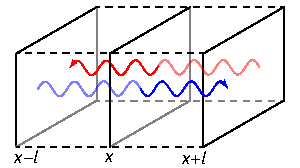
\includegraphics[width=\linewidth]{diffusive-flux}
\caption{\label{f.diffusive-flux} Illustration of net flux crossing a face between regions with slightly different energy densities.}
\end{marginfigure}

\begin{exercisebox}[Rosseland weighting]
Compare this crude diffusion model,
\[
	F = -\frac{1}{3}c\lambda\DD{U}{r},
\]
with eq.~(\ref{e.radiative-transfer}). Using the results of exercise~\ref{ex.radiative-transfer}, give a succinct description for why the effective mean free path $\lambda = 1/(\rho\kappa_{\mathrm{R}})$ is computed using a weighting function $\partial B_{\nu}/\partial T$.
\end{exercisebox}

\begin{marginfigure}
\includegraphics[width=\linewidth]{random-walk-schematic}
\caption{\label{f.random-walk-schematic}Schematic of a random walk of 50 steps.}
\end{marginfigure}
\newthought{As an alternate take on our estimation, let's model the transport as a photon that is randomly walking throughout the interior.}
The photon moves at speed $c$, but it can only go one mean free path $\lambda$ before being absorbed or scattered, at which point it is sent off in a random direction.\marginnote{To keep things simple, we'll imagine that after absorption the atom immediately emits an identical photon in a random direction.} The path of the photon will therefore look something like that in Fig.~\ref{f.random-walk-schematic}.

We will just do our calculation for motion along a diameter, with the photon starting at the center. At each hop, the photon either goes left or right with equal probability. On average, the photon doesn't go anywhere; but after enough hops, there is some probability for the photon to reach the edge of the star and escape. Figure~\ref{f.random-walk} shows the distribution of positions for walks of length $n = 10, 30, 100, 300$ steps, with each step having length 1.0. Suppose the edge of the star is at $x=\pm 10$ (red dotted lines).  Although the average position is at $x=0$, for $n \gtrsim 100$ steps, there is a reasonable probability of the photon escaping.
\begin{figure}[htbp]
\forceversofloat
\includegraphics[width=\linewidth]{random-walk}
\caption{\label{f.random-walk} Distribution of positions after $n$ steps in a random walk.}
\end{figure}

To make this into a workable model, let us first recall the basic features of a random walk. It is described by a binomial distribution: after $n$ steps, the probability that $m$ of them were to the right is
\begin{equation}\label{e.binomial}
    \binom{n}{m}{p} = \frac{n!}{m!(n-m)!} p^{m}(1-p)^{n-m}.
\end{equation}
Here $p$ is the probability of any single step being to the right.
The mean and root variance of $m$ are
\begin{eqnarray}
	\mean{m} &=& np \label{e.mean-binomial} \\
	\left[\mean{\left(m-\mean{m}\right)^{2}}\right]^{1/2} &=& \left[np(1-p)\right]^{1/2}. \label{e.var-binomial}
\end{eqnarray}
We can use these to estimate the diffusion timescale $\tau$.

\begin{exercisebox}[Radiative diffusion as a random walk]
\begin{enumerate}
\item
Show from equation~(\ref{e.mean-binomial}) that the mean distance traveled by the photon after $n$ steps is $\langle d\rangle = \lambda(2np-n)$, so for $p=1/2$, $\langle d\rangle = 0$.

\item
If all the steps were in the same direction, how many steps are needed to reach the edge, at a a distance $R$ from the center? Assume all steps have the same length $\lambda$.

\item\label{p.straight-line-steps}
We want the distribution of steps (cf.\ Fig.~\ref{f.random-walk}) to be wide enough to reach the edge. Set the root variance---a measure of the width of the probability distribution---equal to this number of steps in part~\ref{p.straight-line-steps}, and use equation~(\ref{e.var-binomial}) to find $n_{\mathrm{edge}}$ in terms of $R$ and $\lambda$.

\item
What is the \emph{total} distance traveled by the photon after $n_{\mathrm{edge}}$ steps? If the photon traveled at speed $c$, how long did it take? Compare your answer with that for part~\ref{p.tau} of exercise~\ref{ex.radiative-transfer-diffusion}.

\end{enumerate}
\end{exercisebox}


\chapter{Edge of Darkness}\label{ch.stellar-atmospheres}
% !TEX root = ../intro-stellar-physics.tex

We are now ready to investigate heat transport near the edge, where the optical depth $\tau_{\nu} \lesssim 1$ and photons begin to freely escape. We can no longer use the approximation of radiative diffusion, because conditions in the star are now changing over distances of a mean free path. Let's return to equation~(\ref{e.transfer-equation}) for radiative transport:
\[
	\DD{I_{\nu}}{s} = -\rho\left(\kapabs + \kapscat\right) I_{\nu} + \rho j_{\nu} + \rho\kapscat J_{\nu}.
\]
In general, this is difficult to solve: for some frequencies, the atmosphere will be nearly transparent, while for other frequencies it is quite opaque. Rather than develop the numerical machinery to solve the equation, we shall adopt a simple approximation that will allow us to obtain an approximate solution for the temperature of the stellar atmosphere.

\marginnote[\baselineskip]{\colorbox{yellow}{\textbf{Assumption: Grey opacity}}}We assume that the opacity is gray. That is, the opacity is independent of frequency. This is unphysical, but the solutions for temperature and pressure will have the correct overall behavior.

We next must define a coordinate system. Since we are in a thin layer near the edge of the star, we will adopt planar coordinates, with $z$ being the altitude above some point. We'll pick $z=0$ to be a point deep enough in the star that $I_{\nu}\approx B_{\nu}$. Then we define the optical depth as
\begin{equation}\label{e.optical-depth-planar}
	\tau = \int_{z}^{\infty} \rho\left(\kappa^{\mathrm{abs}}+\kappa^{\mathrm{sca}}\right)\,\dif z ;
\end{equation}
differentiating this expression gives
\[
	\DD{\tau_{\nu}}{z} = -\rho\left(\kappa^{\mathrm{abs}}+\kappa^{\mathrm{sca}}\right).
\]
Note the ``$-$'': in these coordinates, as $z$ gets larger, $\tau$ gets smaller.

We may rewrite the equation (\ref{e.hydrostatic-equilibrium-g}) of hydrostatic balance as
\begin{eqnarray}
	-\rho g = \DD{P}{z} &=& \DD{P}{\tau}\DD{\tau}{z} = -\rho\kappa,\nonumber\\
	\DD{P}{\tau} &=& \frac{g}{\kappa}.
\label{e.P-tau}
\end{eqnarray}
Since we are in a thin layer, we can take the gravitational acceleration $g$ as being approximately constant. Integrate hydrostatic equilibrium to where $\tau = 1$, and if $\kappa$ is approximately constant over this layer,
\[
	P_{\mathrm{ph}} = \int_{0}^{P_{\mathrm{ph}}}\,\dif P = \int_{0}^{1}\frac{g}{\kappa}\,\dif\tau \approx \frac{g}{\kappa}.
\]
\emph{The surface gravity sets the pressure at the \textbf{photosphere}, the location where the optical depth is of order unity and where photons can escape from the star.}

\begin{exercisebox}[Photospheric pressure]
Suppose you observe a star that has a 10\% larger mass and 10\% larger radius than the Sun. All else being equal, how does the pressure at the photosphere of this star compare to that of the Sun?
\end{exercisebox}

\marginnote[\baselineskip]{\colorbox{yellow}{\textbf{ASSUMPTION: Steady-state, LTE}}}
Next, we assume that the matter is in \newterm{local thermal equilibrium} (LTE). This means there is a well-defined temperature at each depth. Furthermore, the emissivity is related to the absorption opacity,
\[
	j_{\nu} = \kappa^{\mathrm{abs}}B_{\nu}.
\]
Note that this does \emph{not} imply anything about the radiation field. We can now take the radiative transfer equation (\ref{e.transfer-equation}) and substitue our definition of optical depth (eq.~[\ref{e.optical-depth-planar}]) to obtain
\begin{equation}\label{e.transfer-gray}
	\mu\DD{I_{\nu}}{\tau} = I_{\nu} - S_{\nu}.
\end{equation}
Here
\[
	S_{\nu} = \frac{j_{\nu} + \kappa^{\mathrm{sca}} J_{\nu}}{\kappa}
	= \frac{\kappa^{\mathrm{abs}} B_{\nu} + \kappa^{\mathrm{sca}} J_{\nu}}{\kappa}.
\]
If, in addition, the matter is in steady-state, then the rate at which energy is absorbed from the radiation field, $\int\kappa^{\mathrm{abs}}I_{\nu}\,\dif\nu\,\dif\Omega$, must equal the rate at which energy is emitted, $\int j_{\nu}\,\dif\nu\,\dif\Omega$. Since we are in LTE,
\[
	\int \left(j_{\nu} - \kappa^{\mathrm{abs}}I_{\nu}\right)\,\dif\nu\,\dif\Omega
	= 4\pi\kappa^{\mathrm{abs}}\int\left(B_{\nu} - J_{\nu}\right)\,\dif\nu = 0.
\]
The average intensity, $J_{\nu} = (4\pi)^{-1}\int I_{\nu}\,\dif\Omega$ may not be equal to $B_{\nu}$, but it has to balance when integrated over all angles.

Let's use this: integrate equation~(\ref{e.transfer-gray}) over all angles and frequencies. Since $\tau$ is gray, we can pull the derivative out from the integral,
\begin{eqnarray*}
	\DD{}{\tau}\int \mu I_{\nu}\,\dif\nu\,\dif\Omega &=& \int I_{\nu}\,\dif\nu\,\dif\Omega - \frac{\kappa^{\mathrm{abs}}}{\kappa}\int B_{\nu}\,\dif\nu\,\dif\Omega - \frac{\kappa^{\mathrm{sca}}}{\kappa} \int J_{\nu}\,\dif\nu\,\dif\Omega\\
	\DD{}{\tau}\int F_{\nu}\,\dif\nu &=& \frac{4\pi}{\kappa}\left[
		(\kappa^{\mathrm{abs}}+\kappa^{\mathrm{sca}})\int J_{\nu}\,\dif\nu
		- \kappa^{\mathrm{abs}}\int B_{\nu}\,\dif\nu
		- \kappa^{\mathrm{sca}}\int J_{\nu}\,\dif\nu\right]\\
	&=& 4\pi\frac{\kappa^{\mathrm{abs}}}{\kappa}\int\left(J_{\nu}-B_{\nu}\right) = 0.
\end{eqnarray*}
Here we used $\kappa = \kappa^{\mathrm{abs}}+\kappa^{\mathrm{sca}}$ to simplify the right-hand side.

\newthought{We have our first result!} For a steady-state gray atmosphere in local thermal equilibrium, the total flux $F = \int F_{\nu}\,\dif\nu$ is constant. The radiative energy is just passing through. Looking at equation (\ref{e.transfer-gray}), you might notice that if we multiplied by $\mu$ and integrated over all frequencies and angles, then we would have an expression for $F$. Let's try that:
\[
	\DD{}{\tau}\int\mu^{2}I_{\nu}\,\dif\nu\,\dif\Omega = F - \int \mu S_{\nu}\dif\nu\,\dif\Omega = F.
\]
The last term vanishes because $S_{\nu}$ is independent of angle and $\int_{0}^{2\pi} \cos\theta\,\sin\theta\,\dif\theta = 0$.  The term on the left-hand side is just $c\,\dif\Prad/\dif\tau$, where $\Prad$ is the radiation pressure (Box~\ref{sb.radiation-pressure}). Since $F$ is constant, we can integrate this equation to obtain
\[
	c\Prad = F(\tau + \tau_{0}),
\]
where $\tau_{0}$ is an integration constant.

\begin{sidebar}[Momentum transport and radiation pressure]
\label{sb.radiation-pressure}
In chapter~\ref{ch.starlight} we defined the flux and radiative energy density, and related both the the intensity $I_{\nu}$. You will learn in your quantum mechanics course that the momentum of a photon of energy $h\nu$ traveling along direction $\unitk$ is
\[ \bvec{p} = \frac{h\nu}{c}\unitk = \frac{h}{\lambda}\unitk. \]
Here $\nu$ and $\lambda = c/\nu$ are the frequency and wavelength of the photon. If we now have a ray of light with intensity $I_{\nu}$ traveling along $\unitk$, then $I_{\nu}$ is the amount of energy carried by photons per area per time along the direction $\unitk$. Hence the momentum transported by those photons per area per time along direction $\unitk$ is $(I_{\nu}/c)\unitk$.

Now suppose we have a sheet of absorbing material with a normal $\unitn$. As the photons are absorbed, they transfer to momentum to the material. The rate of momentum transfer per area is
\begin{eqnarray}
P_{\nu} &=& \frac{1}{c}\int I_{\nu}
	{\color{red}\underbrace{\left(\unitn\vdot\unitk\right)}_{\textrm{proj.~area}}}
	{\color{blue}\underbrace{\left(\unitn\vdot\unitk\right)}_{\textrm{comp.\ of $\bvec{p}$ along $\unitn$}}}
	\,\dif\Omega \nonumber\\
	&=& \frac{1}{c}\int_{0}^{2\phi}\int_{-1}^{1}I_{\nu} \mu^{2}\,\dif \mu\,\dif\phi.
\label{e.momentum-transfer}
\end{eqnarray}
A change in momentum per time is a force; hence equation~(\ref{e.momentum-transfer}) represents the force per area, or \newterm{pressure}, exerted by photons with frequencies in $[\nu,\nu+\dif\nu]$ on the material. The two factors of $\mu=\cos\theta$ account for the projected area and the component of momentum along the normal to the surface $\unitn$.

If the radiation is thermal, then $I_{\nu} = B_{\nu}$, which is independent of angle. Hence
\[
	P_{\nu} = \frac{4\pi}{3c}B_{\nu},
\]
and we can integrate over frequency to get the total pressure,
\begin{equation}\label{e.radiation-pressure}
	\Prad = \frac{4\pi}{3c}\int_{0}^{\infty}B_{\nu}\,\dif\nu = \frac{4}{3c}\sigmaSB T^{4} = \frac{1}{3}aT^{4}.
\end{equation}
Note that the pressure is $1/3$ of the energy density. This is in general true for a gas of relativistic particles that have momentum proportional to energy.
\end{sidebar}

By itself, the expression for the radiation pressure doesn't help: we have an additional equation, but also an additional unknown, namely $\Prad$. But notice! At great depths, where $I_{\nu}\to B_{\nu}$, we have (eq.~[\ref{e.radiation-pressure}]) $\Prad = aT^{4}/3 = (4\pi/3c)J$, where $J=\int J_{\nu}\,\dif\nu$. In desperation, we might try the assumption that this holds everywhere. This assumption is clearly wrong; but desperation often masquerades as genius. Our desperate act is equivalent to expressing the intensity as a \emph{linear} function in $\cos\theta$, which looks like a reasonable approximation scheme, and is in fact called the \emph{Eddington approximation.}
\marginnote{\colorbox{yellow}{\textbf{APPROXIMATION: intensity is linear in $\mu$}}}

Going back to our starting equation (\ref{e.transfer-gray}), we can integrate over all frequencies. Since $\int(J_{\nu}-B_{\nu})\,\dif\nu = 0$, it is easy to show that $S = J$, where $S=\int S_{\nu}\,\dif\nu$. But $J = 3c\Prad/4\pi = (3/4\pi)F(\tau + \tau_{0})$, and so eq.~(\ref{e.transfer-gray}) becomes
\[
	\mu \DD{I}{\tau} = I -\frac{3}{4\pi} F (\tau +\tau_{0}).
\]
This is a first-order ordinary differential, and is easily solved. The solution is
\[
	I(\mu,\tau=0) = \frac{3}{4\pi}F(\mu + \tau_{0})
\]
Now, at $\tau=0$, all of the radiation is outward-bound ($0\le\mu\le 1$). So let's integrate this equation,
\[
	F = 2\pi\int_{0}^{1}\mu I(\mu,\tau=0)\,\dif\mu = \frac{3}{2}F\int_{0}^{1} (\mu^{2} + \mu\tau_{0}),\dif\mu = F\left(\frac{1}{2} + \frac{3}{4}\tau_{0}\right).
\]
This fixes $\tau_{0} = 2/3$.

Now we can assemble all of the pieces and wrap up this long derivation. Since the total flux $F$ is constant, we can set it to its value at $\tau=0$, namely $F = \sigmaSB\Teff^{4}$. Then we can write $\Prad = (1/3) a T^{4}$ and use our solution $c\Prad = F(\tau+\tau_{0})$ along with the relation $\sigmaSB = ac/4$ to obtain
\begin{equation}\label{e.T-tau}
T^{4} = \frac{3}{4}\Teff^{4}\left(\tau + \frac{2}{3}\right).
\end{equation}
This equation, along with eq.~(\ref{e.P-tau}), determines the structure of the stellar atmosphere.

\section{Whatever this is}
You may recall from electrostatics that we can decompose the field from a set of charges into a sum of moments: dipole, quadrupole, and so on. The basis functions for this are the Legendre polynomials $\Pl{n}(\cos\theta)$, defined by the expansion
\begin{equation}
	\frac{1}{\sqrt{1 - 2\mu z + z^{2}}} = \sum_{n=0}^{\infty}\Pl{n}(\mu)z^{n},
\end{equation}
for $-1<\mu<1,\;|z| < 1$. The first three polynomials are
\begin{eqnarray}
	\Pl{0}(\mu) &=& 1 \nonumber\\
	\Pl{1}(\mu) &=& \mu \nonumber\\
	\Pl{2}(\mu) &=& \frac{1}{2}(3\mu^{2}-1).
\end{eqnarray}
The first eight Legendre polynomials are plotted below.

\begin{figure*}
\includegraphics[width=\linewidth]{legendre}
\caption[Legendre polynomials]{\label{f.legendre}
Polar plots of $\Pl{n}(\cos\theta)$ for $n=0,\ldots,7$.}
\end{figure*}

The Legendre polynomials are \emph{orthogonal} in the following sense:
\begin{equation}\label{e.orthogonal}
\int_{-1}^{1}\Pl{n}(\mu)\Pl{m}(\mu)\dif \mu = \left\{
\begin{array}{lr}
	0 &  m\neq n\\
	\frac{2}{2n+1} & m=n
\end{array}\right..
\end{equation}
As a result, we can decompose the radiative intensity into multipoles:
\begin{equation}\label{e.decomposition}
	I = \sum_{n=0}^{\infty} I_{n} \Pl{n}(\mu).
\end{equation}
As $n$ increases, the angular scale of variations becomes finer.

\newthought{To take moments of the intensity}, notice that we can write the weighting factors in terms of Legendre polynomials:
\begin{eqnarray*}
	J &=& \frac{1}{4\pi}\int\,\dif\phi\dif\mu\,{\color{red}\mu^{0}}\,I 
		= \frac{1}{2}\int_{-1}^{1}\dif\mu\sum_{n=0}^{\infty} \,{\color{red}\Pl{0}} I_{n} \\
	H &=& \frac{1}{4\pi}\int\,\dif\phi\dif\mu\,{\color{red}\mu^{1}}\,I 
		= \frac{1}{2}\int_{-1}^{1}\dif\mu\sum_{n=0}^{\infty} \,{\color{red}\Pl{1}} I_{n} \\
	K &=& \frac{1}{4\pi}\int\,\dif\phi\dif\mu\,{\color{red}\mu^{2}}\,I 
		= \frac{1}{2}\int_{-1}^{1}\dif\mu\sum_{n=0}^{\infty} \,{\color{red} \frac{1}{3}(2\Pl{2}+\Pl{0})} I_{n}
\end{eqnarray*}
Now we can use the orthogonality relation (eq.~[\ref{e.orthogonal}]) to compute the integrals:
\begin{eqnarray*}
	J &=& I_{0} \\
	H &=& \frac{1}{3}I_{1} \\
	K &=& \frac{1}{3}\left(\frac{2}{5}I_{2} + I_{0}\right)
		= \frac{1}{3}\left(\frac{2}{5}I_{2} + J\right)
\end{eqnarray*}
Applying the Eddington approximation, i.e., setting $K = J/3$, means that we must set $I_{2} = 0$. Once we do this, we can solve for $J$, $H$, and $K=J/3$ as functions of optical depth $\tau$. This gives us a description of the radiative intensity in terms of $J(\tau)$ and $H$,
\[
	I(\tau,\mu) = J(\tau) + 3H \Pl{1}(\mu) + \cdots \approx J(\tau) + 3H\cos\theta,
\]
which neglects the higher order terms $I_{n}\Pl{n},\forall n > 2$.

\newcommand*{\DDtt}[1]{\frac{\dif^{2} #1}{\dif t^{2}}}
\newcommand*{\wt}{\omega t}
\newcommand*{\wot}{\omega_{0} t}
\newcommand*{\wmt}{\omega_{m} t}
\newcommand*{\womw}{(\omega_{0}^{2}-\omega^{2})}
\newcommand*{\gw}{\Gamma^{2}\omega^{2}}

\nocite{Mihalas1978Stellar-Atmosph,LeBlanc2010An-Introduction,Carroll2006An-Introduction}

\section{Atomic Lines}

Let's begin with a simple system: a mass $m$ attached to a spring with force constant $k$ as shown in Fig.~\ref{f.simple-spring}.

\begin{marginfigure}[-8\baselineskip]
\includegraphics[width=\linewidth]{simple-spring}
\caption[A simple harmonic oscillator]{A simple harmonic oscillator: a mass $m$ on a frictionless surface attached to a  spring with force $F = -kx$.
\label{f.simple-spring}}
\end{marginfigure}

\subsection{With no driving force}

If we put the origin of our coordinate system where the mass is at rest with the spring relaxed, then the equation of motion of the mass is
\begin{equation}\label{e.SHO-basic}
	\DDtt{x} + \frac{k}{m} x = 0.
\end{equation}
You have solved this before: the most general solution is
\begin{equation}\label{e.SHO-general-solution}
	x(t) = x_{0}\cos(\wot) + \frac{v_{0}}{\omega_{0}}\sin(\wot)
\end{equation}
with $\omega_{0}^{2} = k/m$ and with $x_{0}$ and $v_{0}$ being the initial position and velocity of the mass.

\subsection{With driving at frequency $\omega \neq \omega_{0}$}

Now let's push on our mass with an oscillating force, $F\cos(\omega t)$ with $\omega\neq\omega_{0}$. A real world example would be holding a vibrating tuning fork near another fork tuned to a different frequency.  The equation of motion is now
\begin{equation}\label{e.SHO-driven}
	\DDtt{x} + \omega_{0}^{2}x = \frac{F}{m}\cos(\wt).
\end{equation}
You can verify by substitution that a general solution is
\[
	x(t) = \frac{F/m}{(\omega_{0}^{2}-\omega^{2})}\cos(\wt) + A\cos(\wot)+B\sin(\wot).
\]
Let's start with our harmonic oscillator at rest ($v_{0} = \left.\dif x/\dif t\right|_{t=0} = 0$) and at $\left. x\right|_{t=0} = 0$.  With these conditions, we can determine the constants $A$ and $B$; the solution is
\[
	x(t) = \frac{F/m}{(\omega_{0}^{2}-\omega^{2})}\left[\cos(\wt)-\cos(\wot)\right].
\]
Let's recast this by defining $\Delta = \omega_{0} - \omega$ and $\omega_{m} = (\omega_{0}+\omega)/2$.  Then
\begin{eqnarray*}
  \omega_{0}^{2}-\omega^{2} &=& (\omega_{0}-\omega)(\omega_{0}+\omega) = 2\Delta\omega_{m},\\
  \cos(\wot) &=& \cos\left(\wmt+\Delta t/2\right) = \cos(\wmt)\cos(\Delta t/2) - \sin(\wmt)\sin(\Delta t/2),\\
  \cos(\wt) &=& \cos\left(\wmt-\Delta t/2\right) = \cos(\wmt)\cos(\Delta t/2) + \sin(\wmt)\sin(\Delta t/2);
\end{eqnarray*}
and we write the solution as
\begin{equation}\label{e.beats}
	x(t) = \left[\frac{F/m}{\Delta\omega_{m}}\sin(\Delta t/2)\right]\sin(\wmt).
\end{equation}
This illustrates the phenomena of beats: the oscillation consists of a carrier signal at frequency $\omega_{m}$ with the amplitude modulated at the slower frequency $\Delta /2$.  Notice that the amplitude increases as $\Delta \to0$, i.e., $\omega\to\omega_{0}$.

\subsection{With both driving and damping}

Now let's make our model even more realistic by adding some damping.  We add a frictional force that is proportional to velocity, $F_{\mathrm{friction}} = -m\Gamma \dif x/\dif t$. Our complete equation of motion is then
\begin{equation}
	\DDtt{x} + \Gamma \DDt{x} + \omega_{0}^{2}x = \frac{F}{m}\cos(\omega t).
\end{equation}
The solution to this is straightforward to find, although the algebra is tedious (trust me on this). The general solution for initial conditions $\left.x\right|_{t=0} = x_{0}$ and $\left.\dif x/\dif t\right|_{t=0} = v_{0}$ is
\begin{eqnarray}
\label{e.general-solution-ddo}
\lefteqn{x(t) = \frac{F\womw/m}{\womw^{2}+\gw}\cos(\omega t)} && \\
	&+& \frac{\Gamma\omega F/m}{\womw^{2}+\gw}\sin(\omega t)\nonumber \\
	&+& \left[x_{0}-\frac{F\womw/m}{\womw^{2}+\gw}\right]{\color{red}e^{-\Gamma t/2}} \cos(\omega_{\Gamma}t) \nonumber\\
	&+& \left[\frac{v_{0}}{\omega_{\Gamma}}-\frac{\Gamma\omega F/m}{\womw^{2}+\gw}
	\,\frac{\omega}{\omega_{\Gamma}}\right]{\color{red}e^{-\Gamma t/2}} \sin(\omega_{\Gamma}t), 
	\nonumber
\end{eqnarray}
with
\[ 
    \omega_{\Gamma} = 
        \omega_{0}\left(1-\frac{\Gamma^{2}}{4\omega_{0}^{2}}\right)^{1/2}.
\]
Let's simplify this to the most relevant case.  First, the last two terms decay as {\color{red}$e^{-\Gamma t/2}$}: these are transients set by the initial conditions. After a time $2/\Gamma$ there will only be the first two terms, which oscillate at frequency $\omega$. 

We can simplify these first two terms even further: write
\[ \cos(\wt) = \frac{e^{i\wt}+e^{-i\wt}}{2},\quad \sin(\wt) 
    = \frac{e^{i\wt}-e^{-i\wt}}{2i}; \]
and combine terms to find
\begin{eqnarray}
    x(t) &=& \frac{F}{2m}\left[\frac{1}{\left(\omega_0^2-\omega^2\right) + i\Gamma\omega}\right]e^{i\wt} + \frac{F}{2m}\left[\frac{1}{\left(\omega_0^2-\omega^2\right) - i\Gamma\omega}\right]e^{-i\wt} \nonumber\\
    &=& \Re\left\{\frac{F}{m}\left[\frac{1}{\left(\omega_0^2-\omega^2\right) + i\Gamma\omega}\right]e^{i\wt}\right\}\label{e.oscillator-expression}
\end{eqnarray}
We use the symbol ``$\Re$'' to denote taking the real part of a complex quantity.  

From Eq.~(\ref{e.oscillator-expression}), we see that the oscillator can be described as the real part of a complex quantity $Ae^{i\wt}$, with
\[
    A = \frac{F}{m}\left[\frac{1}{\left(\omega_0^2-\omega^2\right) + i\Gamma\omega}\right].
\]
For $\omega \approx \omega_0$, we write $(\omega_0^2-\omega^2)\approx 2\omega_0(\omega_0-\omega)$ and take the square of the amplitude to find,
\begin{eqnarray}
    \left|A\right|^2 &=& \left(\frac{F}{2m\omega_0}\right)^2
        \frac{1}{(\omega_0-\omega)^2 + (\Gamma/2)^2}\nonumber\\
    &=& \frac{\pi}{2\Gamma}\left(\frac{F}{m\omega_0}\right)^2
        \left\{\frac{1}{\pi}\frac{\Gamma/2}{(\omega_0-\omega)^2 + (\Gamma/2)^2}\right\}
\end{eqnarray}
We rewrote the amplitude in the second line so that the term in $\{\cdot\}$ is normalized. The function
\[
    \mathcal{L}(\omega;\Gamma) = \frac{1}{\pi} 
        \frac{\Gamma/2}{(\omega_0-\omega)^2 + (\Gamma/2)^2}
\]
is known as a Lorentzian.  In contrast to a Gaussian, a Lorentzian is characterized by broad ``wings'' (Fig.~\ref{f.comparison}) as it goes to zero away from the central frequency $\omega_{0}$.
\begin{marginfigure}[-4\baselineskip]
\includegraphics[width=\linewidth]{comparison}
\caption[Comparison of Lorentzian and Gaussian distributions]{\label{f.comparison}
Comparison of a Lorentzian ($\mathcal{L}$, solid line) and a Gaussian ($\mathcal{G}$, dotted line), both with $\mathrm{FWHM}=1$. The area under each curve is unity.}
\end{marginfigure}

\section{Atomic Lines}
You may be thinking, ``What does this have to do with atomic lines?'' Consider an electronic transition in an atom between two energy levels, $E_m$ and $E_n$. The natural frequency of this transition is $\nu_0 = |E_n-E_m|/h$. Light incident on the atom with frequency\sidenote{We are switching from angular frequency $\omega$ to frequency $\nu = \omega/2\pi$.} $\nu\neq\nu_0$ drives the electron at frequency $\nu$. An accelerating electron radiates, which damps the acceleration of the electron.  Classically, the transition in an atom is an electromagnetic oscillator with damping and driving terms, with cross-section\sidenote{For details, see the Box~\ref{b.line-emission}.}
\begin{equation}\label{e.semi-classical}
    \sigma = \left(\frac{\pi e^2}{m_e c}\right)
    \left\{\frac{\Gamma/4\pi}{(\nu_0-\nu)^2 + (\Gamma/4\pi)^2}\right\}.
\end{equation}
The actual value of the cross-section must be calculated using quantum mechanics. The overall shape of the cross-section is still in the form of equation~(\ref{e.semi-classical}) with opacity
\begin{equation}
    \rho\kappa_\nu = n_i \left(\frac{\pi e^2}{m_e c}\right) f_{mn}
        \left\{\frac{\Gamma/4\pi}{(\nu_0-\nu)^2 + (\Gamma/4\pi)^2}\right\}.
\end{equation}
In this equation, $f_{mn}$ is a number, called the \emph{oscillator strength}, that results from the calculation of the transition probability from state $m$ to state $n$, and $n_i$ is the density of atoms in state $m$.  The key point is that $f_{mn}$ depends only on the details of the transition: the energies, spins, and parities of the atomic states.  It does not depend on environmental parameters such as temperature and pressure.  As a result, $f_{mn}$ can be measured or computed once and then tabulated.


\begin{sidebar}[Treating line emission as a driven damped oscillator]
\label{b.line-emission}
NB. In this box, Gaussian CGS units are used for the electromagnetic field. To convert to MKS, make the following substitutions:
\begin{eqnarray*}
e &\to& \frac{1}{\sqrt{4\pi\varepsilon_0}}e\\
\bvec{E} &\to& \sqrt{4\pi\varepsilon_0}\bvec{E}\\
c &\to& (\mu_0\varepsilon_0)^{-1/2}.
\end{eqnarray*}

\newthought{Suppose we have a classical charged harmonic oscillator.}  The instantaneous power emitted by the oscillator is
\begin{equation}\label{e.larmor-power}
	 P(t) = \frac{2}{3}\frac{e^{2}}{c^{3}} |\dot{\vu}|^{2},
\end{equation}
and when averaged over a cycle is
\begin{equation}\label{e.oscillator-power}
	 \left\langle P(t) \right\rangle = \frac{e^{2}}{3c^{3}}x_{0}^{2} \omega^{4},
\end{equation}
since $\dot{\vu} = -\omega^{2}\bvec{x}_{0}\cos \omega t$. Since the oscillator is radiating, it is losing energy and is damped. Let us write the damping as $\bvec{F}_{\mathrm{rad}}\vdot \vu$; to find $\bvec{F}_{\mathrm{rad}}$, we integrate the power loss over a cycle,
\[  -\int_{t_{1}}^{t_{2}}\!\dif t\;\frac{2}{3}\frac{e^{2}}{c^{3}}\dot{\vu}\vdot\dot{\vu} 
	= -\left.\frac{2}{3}\frac{e^{2}}{c^{3}}\dot{\vu}\vdot\vu\right|_{t_{1}}^{t_{2}} 
	+ \frac{2}{3}\frac{e^{2}}{c^{3}} \int_{t_{1}}^{t_{2}}\!\dif t\;\ddot{\vu}\vdot\vu. 
\]
Since the motion is periodic, the first term vanishes and we can therefore identify 
\[ 
	\bvec{F}_{\mathrm{rad}} = \frac{2}{3}\frac{e^{2}}{c^{3}}\ddot{\vu} 
	= -m\left(\frac{2e^{2}\omega^{2}}{3c^{3}m}\right)\vu
\]
as the radiation damping term with the term in parenthesis being the damping constant $\gamma$. 
If there is an driving electric field on our oscillator, then its equation of motion becomes
\begin{equation}\label{e.eq-sho}
	m\ddot{\bvec{x}} = -m\omega_{0}^{2}\bvec{x} + e\bvec{E}e^{i\omega t} - m\gamma \dot{\bvec{x}}.
\end{equation}
Using a trial function $\bvec{x}\propto e^{i\omega t}$ gives
\[
	\bvec{x} = \frac{e}{m}\frac{E e^{i\omega t}}{(\omega_{0}^{2}-\omega^{2}) + i\omega\gamma}.
\]
Taking the second derivative w.r.t.\ time of $\bvec{x}$, substituting into eq.~(\ref{e.larmor-power}), and averaging over a cycle gives the power radiated by the oscillator,
\[
	\left\langle P(t)\right\rangle = \frac{e^{4}\omega^{4} E^{2}}{3 c^{2}m^{2}}
	\frac{1}{(\omega_{0}^{2}-\omega^{2})^{2} + \gamma^{2}\omega^{2}}.
\]
Dividing $\langle P(t)\rangle$ by the incident power per unit area, $cE^{2}/(8\pi)$, gives the cross-section:
\begin{equation}\label{e.classical-oscillator-cross-section}
	\sigma = \frac{8\pi}{3}\frac{e^{4}}{m^{2}c^{3}}
	\frac{\omega^{4}}{(\omega_{0}^{2}-\omega^{2})^{2} + \gamma^{2}\omega^{2}}.
\end{equation}
Now, for $\omega \approx \omega_{0}$, we can expand $(\omega_{0}^{2}-\omega^{2})^{2} \approx 4\omega_{0}^{2}(\omega_{0}-\omega)^{2}$; furthermore, we identify $2e^{2}\omega_{0}^{2}/(3c^{3}m) = \gamma$ and equation~(\ref{e.classical-oscillator-cross-section}) becomes
\begin{equation}\label{e.cross-section-lorentz}
	\sigma = \pi\left(\frac{e^{2}}{mc}\right)\frac{\gamma}{(\omega_{0}-\omega)^{2} + (\gamma/2)^{2}}.
\end{equation}
The line profile is Lorentzian, with a width $\gamma$. In terms of wavelength, the width is
\[ 
	\Delta \lambda = \left|\frac{\dif\lambda}{\dif\omega}\right|\gamma = \frac{2\pi c}{\omega^{2}}\gamma
	= \val{\sci{1.2}{-4}}{\textrm{\AA}}.
\]
This width is independent of the transition frequency (it is just the classical electron radius), and it is very, very small.  In a stellar atmosphere, the width is set by interactions and doppler broadening.

\newthought{To understand how impacts affect the line width}, suppose we model the oscillator as being started and stopped by impacts; in between impacts it just goes as $e^{i\omega_{0}t}$.  To get the spectrum, we take the Fourier transform,
\[
	F(\omega,t) = \int_{0}^{t}\!\dif t'\; \exp[i(\omega_{0}-\omega)t'],
\]
where $t$ is some time between impacts. Now if the impacts are distributed randomly and are uncorrelated, then the distribution of wait times follows a Poisson distribution,
\[ W(t)\,\dif t = e^{-t/\tau}\,\dif t/\tau, \]
where $\tau$ is the average time between collisions.  Using this to compute the energy spectrum, we obtain
\[ E(\omega) = \frac{1}{2\pi\tau}\int_{0}^{\infty}\!\dif t\; F(\omega,t)F^{*}(\omega,t)W(t) = \frac{1}{\pi\tau} 
	\frac{1}{(\omega_{0}-\omega)^{2} + (1/\tau)^{2}};
\]
the line profile is again Lorentzian, with a FWHM $2/\tau$.
\end{sidebar}



\chapter{A Sky Full of Stars}\label{ch.classifying-stars}
% !TEX root = ../intro-stellar-physics.tex

\nocite{Mihalas1978Stellar-Atmosph,LeBlanc2010An-Introduction,Carroll2006An-Introduction}

To recap, we have established a description for the basic features of a self-gravitating fluid:
\begin{enumerate}

\item For a set mass and radius, hydrostatic equilibrium (balance of pressure and gravity) is established on the time needed for a sound wave to cross the star. Once this equilibrium is established, the central pressure, density, and temperature are established.

\item The gradient in temperature from center to surface drives a luminosity, which is controlled by the opacity of material in the stellar interior.

\item The ambient pressure and temperature near the stellar photosphere (where $\tau \sim 1$) are set by the surface gravity and opacity.

\end{enumerate}

What we haven't established---yet---is how the luminosity is generated: if nuclear reaction are not operating, then the star must contract (on a Kelvin-Helmholtz timescale) until the central temperature is sufficiently hot for reactions to generate the required luminosity.
Before discussing this, however, we shall explore how the emergent spectra of stars serve as diagnostic indicators of ambient conditions in the stellar photosphere. 

\section{Overview}

If light from the Sun is passed through a grating (a piece of glass with finely etched lines), the light is dispersed in wavelength and creates a spectrum, such as the highly detailed one show in Fig.~\ref{f.solar-spectrum}. 
\begin{marginfigure}
\includegraphics[width=\linewidth]{sunsqa}
\caption[Visible spectrum of the sun]{\label{f.solar-spectrum} Visible spectrum of the Sun. Wavelength increases along a row from left to right, and by rows from bottom to top. \emph{Credit:
N.A.Sharp, NOAO/NSO/Kitt Peak FTS/AURA/NSF.}}
\end{marginfigure}
Superposed on the slow variation from red to violet are dark \newterm{absorption lines}. The ions, atoms, and molecules in the solar atmosphere absorb light at specific frequencies and create these lines.

Beginning in the late 1800's, astronomers began classifying stars by the observed absorption lines in the spectra. At this time, Edward Pickering and Williamina Fleming of the Harvard College Observatory began amassing a vast catalog of stellar spectra. They classified these spectra according to the strength of observed hydrogen Balmer lines (the first four are H$\alpha$: \val{657}{\nano\meter}; H$\beta$: \val{486}{\nano\meter}; H$\gamma$: \val{434}{\nano\meter}; H$\delta$: \val{410}{\nano\meter}). Stars, such as Vega, with the strongest Balmer lines were classified as type ``A'', those with the next strongest were type ``B'', and so forth. Annie Jump Cannon, who would later succeed Fleming as curator of astronomical photography at the observatory, simplified and reorganized the scheme, and added decimal subdivisions ($0\ldots9$) for each type\sidenote{For example, the Sun's type is G2}. When stellar color is taken into account, the ordering of stars, from blue to red, is ``OBAFGKM''. In the 1990's the ``L'' and ``T'' classes were added\cite{Kirkpatrick1999Dwarfs-Cooler-t} for cool stars and brown dwarfs (stellar-like objects that do not reach central temperature sufficient for fusion of hydrogen into helium).

Hertzsprung and Russell independently noticed that most stars tended to lie along a band, termed the \newterm{main sequence}, in a plot of absolute magnitude (or luminosity) against stellar type (now known as a \newterm{Hertzsprung-Russell diagram}). Figure~\ref{f.HR} shows some standard main-sequence stars, along with their stellar type and approximate color.
\begin{marginfigure}
\includegraphics[width=\linewidth]{HR}
\caption[Hertzsprung-Russell diagram of standard main-sequence stars]{\label{f.HR} Hertzsprung-Russell diagram showing standard main-sequence stars. Colors are approximate translations of the spectra.}
\end{marginfigure}

In an influential PhD thesis, Cecilia Payne-Gaposhkin\cite{Payne1925Stellar-Atmosph} applied the Boltzmann and Saha equations to show that different stellar spectra were consistent with changes in temperature, rather than composition, of the stellar photosphere. The sequence of stellar types is therefore a temperature sequence, with ``O'' stars being the hottest. 

\section{The hydrogen atom}

To understand why the Balmer lines are strongest in a certain range of temperatures, we first need to review the workings of a hydrogen atom.

The electrons bound to an atom or molecule can only occupy states having a discrete set of energies. For example, the electron in a hydrogen atom only has energies
\begin{equation}\label{e.H-levels}
        E_{n} = -\val{13.6}{\eV}\times \frac{1}{n^{2}},
\end{equation}
where $n > 0$ is an integer known as the \newterm{principal quantum number}.  These energies are negative, relative to a free electron.  For example, the ground state ($n=1$) has energy $-\ERy = -\val{13.6}{\eV}$, meaning that \val{13.6}{\eV} is required to remove an electron in its ground state from the atom.

Because the electrons in an atom can only have certain energies, the atom can only absorb or emit light at specific wavelengths, such that the energy of the photon matches the difference in energy between two levels. For example, a hydrogen atom in its ground state can absorb a photon of energy
\[
        E_{1\to2} = -\ERy \left(\frac{1}{2^{2}} - \frac{1}{1^{2}}\right)
                 = \val{10.2}{\eV}
\]
corresponding to the energy required to excite the electron from level $n=1$ to $n=2$. The wavelengths that can be absorbed by a hydrogen atom at rest can be found by substituting $E = hc/\lambda$ into equation~(\ref{e.H-levels}):
\begin{equation}
        \lambda_{m\to n} = \lambda_{0}\left(\frac{1}{m^{2}}-\frac{1}{n^{2}}\right)^{-1},
\end{equation}
where $\lambda_{0} = \val{91.2}{\nano\meter}$ and $n > m$.
The transitions from the lowest levels are named after their discoverers: Lyman for $1\to n$, Balmer for $2\to n$, Paschen for $3\to n$. A greek letter is used to denote the higher state: for example Lyman $\alpha$ (abbr.\ Ly$\alpha$) means $1\to2$, with $\lambda_{\mathrm{Ly}\alpha} = \val{121.6}{\nano\meter}$. Note that $\lambda_{m\to n} > \lambda_{0}$; photons with wavelengths $\lambda < \val{91.2}{\nano\meter}$ have sufficient energy to knock the electron out of the atom, thereby producing a hydrogen ion and a free electron. The first line transition in the Balmer series is $2\to3$, and is designated H$\alpha$: $\lambda_{\mathrm{H}\alpha} = \val{656.3}{\nano\meter}$. The first 20 lines for each of the Lyman, Balmer, and Paschen series are shown in Fig.~\ref{f.H-spectrum}; note the $3\to4$ transition is outside the plot range. The Balmer lines lie in the visible range.

\begin{marginfigure}[-8\baselineskip]
\includegraphics[width=\linewidth]{H-spectrum}
\caption{Spectral lines of neutral hydrogen 
\label{f.H-spectrum}}
\end{marginfigure}

\section{The Boltzmann Equation}
\label{s.boltzmann-eqn}

In order to produce a Balmer absorption line, we must have some hydrogen atoms in the photosphere with electrons in the energy level $n=2$. The more atoms in a state $n=2$, the more absorption and the stronger the line. To find the number of atoms with energy level $n=2$, we make use of a fundamental result, due to Boltzmann, from statistical (thermal) physics; namely, that if our sample of atoms is in thermal equilibrium, then the ratio of the number of atoms with energy $E_{i}$ to the number of atoms with energy $E_{j}$ is
\begin{equation}\label{e.boltzmann}
\frac{N_{i}}{N_{j}} = \frac{g_{i}}{g_{j}} 
\exp\left(-\frac{E_{i}-E_{j}}{\kB T}\right).
\end{equation}
Here the number $g_{n}$ gives the number\sidenote{$g_{n}$ is known as the \emph{degeneracy} of a given level $n$} of quantum mechanical states having energy $E_{n} = -\ERy/n^{2}$. For an energy level $n$, there are $n^{2}$ possible states, each having a different angular momentum. For each of these $n^{2}$ states, both the electron and proton may each have 2 possible spins. The total number of states for energy $E_{n}$ is therefore $g_{n} = 2\times2\times n^{2}$.

Suppose we wish to know the fraction of atoms in a given state $i$: that is, we wish to know
\[	x_{i} = \frac{N_{i}}{N_{1}+N_{2}+\ldots+N_{i}+\ldots} ? \]
Using equation~(\ref{e.boltzmann}), we can express $x_{i}$ as 
\begin{eqnarray}
  x_{i} &=& \frac{g_{i}e^{-E_{i}/\kB T}}{g_{1}e^{-E_{1}/\kB T}+g_{2}e^{-E_{2}/\kB T}+\ldots+g_{i}e^{-E_{i}/\kB T}+\ldots} \nonumber\\
        &\equiv& \frac{g_{i}e^{-E_{i}/\kB T}}{\pfcn}.
\end{eqnarray}
The quantity 
\begin{equation}\label{e.partition-function}
	\pfcn = \sum_{n} g_{n}\exp\left(-\frac{E_{n}}{\kB T}\right)
\end{equation}
is called the \emph{partition function}: loosely speaking, it indicates the number of ways the sample of atoms can be partitioned among the different energy levels.

\begin{exercisebox}[Partition function for neutral hydrogen]
Assuming that the first term $g_{1}e^{-E_{1}/\kB T}$ dominates the sum in the partition function (see Box~\ref{sb.partition-function}), plot the fraction of neutral hydrogen in its $n=2$ state as a function of temperature, for $\val{5\,000}{\K} < T < \val{20\,000}{\K}$.
\end{exercisebox}

\begin{sidebar}[The partition function for neutral hydrogen]
\label{sb.partition-function}
The partition function for neutral hydrogen, eq.~(\ref{e.partition-function}), has some interesting features. Substituting $g_{n}=4n^{2}$ and $E_{n} = -\ERy/n^{2}$ and factoring out common terms gives
\[	\pfcn = 4e^{\beta\ERy}\sum_{n} n^{2} e^{-\beta\ERy(1-1/n^{2})}, \]
with $\beta = (\kB T)^{-1}$. The sum diverges, since for $n\gg 1$ the individual terms approach $n^{2}e^{-\beta\ERy}$. In practice, this isn't a problem, as there is an upper limit on $n$ set by ambient conditions. For example, the mean distance of the electron from the nucleus is $\approx \abohr n^{2}$, where $\abohr = \val{\sci{5.29}{-11}}{\cm}$ is the Bohr radius. As a result, each atom takes up a volume $\approx \abohr^{3}n^{6}$; if we want the atoms to not overlap, then the volume per atom, $V/N = 1/\xi$, must be larger than this by some factor. Suppose we set that the volume of an atom must be less than half of that available in our gas; then
\[
\xi = \frac{N}{V} < \frac{N}{N\cdot 2\abohr^{3}n^{6}}.
\]
Thus the maximum level is $n < (2\abohr^{3}\xi)^{-1/6}$. For a typical A-star photospheric density $\xi\sim \val{10^{15}}{\cm^{-3}}$, the energy level cutoff is $n \approx 35$. In practice the cutoff will be even lower because of collisions.

The precise maximum value of $n$ is not that important for most applications. The reason is that the terms in the partition function increase only slowly. As an example, the terms and cumulative sum in the partition function at a temperature $T=\val{10^{4}}{\K}$ are as follows.
\begin{center}
\begin{tabular}{rrr}
$n$ & $n^{2} e^{\beta\ERy(1-1/n^{2})}$ & $4\sum_{i=1}^{n} i^{2}e^{-\beta\ERy(1-1/i^{2})}$ \\
\hline
   1 & 1.00e+00 &  4.0000 \\
   2 & 2.88e-05 &  4.0001 \\
   3 & 7.23e-06 &  4.0001 \\
  \multicolumn{3}{c}{\vdots} \\
  26 & 9.62e-05 &  4.0038 \\
  \multicolumn{3}{c}{\vdots} \\
  52 & 3.78e-04 &  4.0274 \\
  \multicolumn{3}{c}{\vdots} \\
 268 & 9.99e-03 &  7.5901 \\
\end{tabular}
\end{center}
As we can see from the cumulative sum (rightmost column), the partition function is insensitive to the precise value of the cutoff until $n$ is quite large; indeed, for many applications it is reasonably accurate to just use the first term: $Q\approx 4e^{\beta\ERy}$. 
\end{sidebar}

\section{Ionization: The Saha equation}
\label{s.saha-eqn}

As the temperature in the gas rises, there are more photons with sufficient energy to eject electrons from an atom. In addition, collisions between atoms also become sufficiently energetic to ionize the atom. In astronomical nomenclature, the ionization state is denoted by a small Roman numeral: \ion{Fe}{i} denotes neutral iron, \ion{Fe}{ii} denotes singly-ionized iron (charge $+1$), \ion{Fe}{iii} denotes doubly-ionized iron (charge $+2$), and so on. In thermal equilibrium, the rate at which atoms are ionized must equal the rate at which ions and electrons recombine: for example, in a gas consisting of hydrogen atoms, hydrogen ions (i.e., protons), and electrons the reaction
\[
	\ion{H}{ii} + e \longleftrightarrow \ion{H}{i}
\]
is in equilibrium. We'd like to extend equation~(\ref{e.boltzmann}) to find the ratio of two ionization states $N_{i+1}/N_{i}$. Although deriving this equation, termed the \newterm{Saha equation}\sidenote{Derived by Meghnad Saha in 1920}, is beyond the scope of the course, what we shall do is take the equation apart and try to understand how it works.  The Saha equation for the ratio of the populations of two ionization states $N_{i+1}$ and $N_{i}$ is
\begin{equation}\label{e.saha}
\frac{N_{i+1}}{N_{i}} 
= {\color{red}\left[\frac{2}{n_{e}}
\left(\frac{2\pi m_{e}\kB T}{h^{2}}\right)^{3/2}\right]}
{\color{blue}\frac{\pfcn_{i+1}}{\pfcn_{i}}}.
\end{equation}
In this equation, $n_{e}$ denotes the electron density---the number of free electrons per unit volume---and $m_{e}$ is the electron mass. The terms $\pfcn_{i+1}$ and $\pfcn_{i}$ are the partition functions for the two states, \emph{both measured with respect to the same zero-point for energy}.

Let's start with the term $\color{blue} Q_{i+1}/Q_{i}$. If both partition functions are dominated by the ground state term\sidenote{see Box~\ref{sb.partition-function}} then
\begin{eqnarray*}
	\frac{Q_{i+1}}{Q_{i}} &=& \frac{g_{i+1,1}}{g_{i,1}} e^{-\beta (E_{i+1,1}-E_{i,1})}\\
	&=& \frac{g_{i+1,1}}{g_{i,1}} e^{-\beta\,E_{\mathrm{ion}}}
\end{eqnarray*}
Here $E_{\mathrm{ion}} = E_{i+1,1} - E_{i,1}$ is the energy needed to remove an electron from an ion in state $i$ and we use the common shorthand $\beta = (\kB T)^{-1}$. Thus $Q_{i+1}/Q_{i}$ resembles equation~(\ref{e.boltzmann}).

The term in $\color{red}\left[\cdot\right]$ in eq.~(\ref{e.saha}) arises because we also need to allow for the number of free electron states. When the atom is ionized, each electron quickly acquires an average kinetic energy $(3/2)\kB T$. There are many different states having this energy: the electron can be in different locations and moving in different directions, for example.  

You might think that there would be an infinitude of possible electron states.  Quantum mechanics, however, sets limitations on this number. First, we have the Pauli exclusion principle: no two electrons can be in the same location with the same momentum and same spin. What do we mean by same location and momentum?  Recall the Heisenberg uncertainty principle: the electrons $x$-position and $x$-momentum are spread about a range of values $\Delta x$ and $\Delta p_{x}$, and these uncertainties are related via
\[ \Delta x\,\Delta p_{x} \gtrsim h. \]
Thus, if we imagine dividing our volume into little boxes of volume
\[ 
 \Delta V = \Delta x\,\Delta y\,\Delta z \approx \frac{h^{3}}{\Delta p_{x}\,\Delta p_{y}\,\Delta p_{z}},
\]
each box can hold two electrons.\sidenote{Because electrons have spin 1/2, we can put two electrons into the same position and momentum state if their spins are oppositely directed.} Suppose we have a volume $V$; how many boxes are there?  The number of available boxes is
\[
	\frac{V}{\Delta V} \approx \frac{V\;\Delta p_{x}\,\Delta p_{y}\,\Delta p_{z}}{h^{3}}.
\]
To estimate the size of $\Delta p_{x}\,\Delta p_{y}\,\Delta p_{z}$, let's take $\Delta p_{x}\sim p_{x}$ and similarly for $\Delta p_{y}$ and $\Delta p_{z}$; further, if everything is isotropic then $p_{x}\approx p_{y}\approx p_{z}$ on average, so $\Delta p_{x}\,\Delta p_{y}\,\Delta p_{z} \sim p_{x}^{3}$.  Now the kinetic energy of the electron is $p^{2}/2m_{e}$, and $p^{2} = p_{x}^{2} + p_{y}^{2} + p_{z}^{2} \approx 3 p_{x}^{2}$. Hence the kinetic energy is $(3/2)p_{x}^{2}/m_{e}$; in thermal equilibrium, however, the kinetic energy has an average value of $(3/2)\kB T$.  The value of $p_{x}^{2}$ is therefore
\[
	p_{x}^{2} \approx m_{e}\kB T,
\]
and the number of boxes is
\[
	\frac{V}{\Delta V} \sim V\frac{p_{x}^{3}}{h^{3}} \sim V\frac{\left(m_{e}\kB T\right)^{3/2}}{h^{3}}.
\]
If our volume $V$ contains $N_{e}$ electrons, then the number of states electron is
\[
	\frac{2V}{N_{e}\Delta V} \sim \frac{2V}{N_{e}}\frac{\left(m_{e}\kB T\right)^{3/2}}{h^{3}}.
\]
The factor of 2 appears because each box can hold 2 electrons.  Recognizing that $N_{e}/V = n_{e}$, we see that this number of states per free electrons corresponds to the factor in $\color{red}\left[\;\right]$ in equation~(\ref{e.saha}). When the numerical calculation is done correctly, the additional factor of $2\pi$ arises.

The number of states per free electron plays an important role in setting the temperature at which a species ionizes. You might expect, since a term $e^{-E_{\mathrm{ion}}/\kB T}$ appears in the ratio $N_{i+1}/N_{i}$, that a species would ionize at a temperature $E_{\mathrm{ion}}/\kB$. In fact the ionization temperature is much lower. To see how this works, define
\[
	\zeta = \ln\left[\frac{1}{n_{e}}\left(\frac{2\pi m_{e}\kB T}{h^{2}}\right)^{3/2}\right].
\]
We can then write eq.~(\ref{e.saha})---with the approximation that the partition functions are dominated by the ground state---as
\[
	\frac{N_{i+1}}{N_{i}} = \frac{2g_{i+1,1}}{g_{i,1}}\exp\left(\zeta - \beta E_{\mathrm{ion}}\right).
\]
Now the factor $g_{i+1,1}/g_{i,1}$ is of order unity. Hence, when the gas ionizes and $N_{i+1,1}\approx N_{i,1}$, we must have that $\zeta\approx \beta E_{\mathrm{ion}}$; put differently, the ionization temperature will not be $E_{\mathrm{ion}}/\kB$ but rather $E_{\mathrm{ion}}/\kB\zeta$. Under conditions in the photosphere of an A star ($T \approx \val{10^{4}}{\K}$, $n\sim \val{10^{15}}{\cm^{-3}}$), $\zeta \approx 15$.

In more intuitive terms, when an electron is ejected from an atom, it has an enormously large number $\sim e^{15}$ number of different states available. To rejoin with an ion requires being in the right place at the right time with the right energy. The large number of available states makes this unlikely, so the electron must wander lonely through a vast and desolate phase space until at long last it reunites with an ion. In a sense, the large number of available states per electron makes ionization easier than recombination; as a result the temperature at which ionization occurs is considerably lower than $E_{\mathrm{ion}}/\kB$.

\begin{exercisebox}[Conditions for strong Balmer lines]
\label{ex.strong-Balmer}
Let $n_{\textsc{i}}$ be the density of \ion{H}{i} and $n_{\textsc{ii}}$ be the density of \ion{H}{ii}. Denote the fraction of neutral hydrogen as $x = n_{\textsc{i}}/(n_{\textsc{i}}+n_{\textsc{ii}})$, so that $1-x = n_{\textsc{ii}}/(n_{\textsc{i}}+n_{\textsc{ii}})$ is the fraction of ionized hydrogen. Take $n_{\textsc{i}}+n_{\textsc{ii}} = \val{10^{15}}{\cm^{-3}}$, and assume that all free electrons come from the ionization of hydrogen, so that $n_{e} = n_{\textsc{ii}}$. Plot $x$ as a function of temperature for $\val{7\,500}{\K}\le T\le \val{15\,000}{\K}$, and find the temperature at which $x = 1/2$. Then multiply $x$ by the fraction $n_{2}/n_{1}$, as set by the Boltzmann equation, to find the fraction of hydrogen in the $n=2$ level.
\end{exercisebox}

As shown in exercise~\ref{ex.strong-Balmer}, the Balmer lines, which correspond to transitions $2\to3$, $2\to 4$, \ldots, are most prominent in A stars. These stars have $\Teff = \valrng[--]{7\,500}{9\,500}{\K}$. At lower temperatures, the population of hydrogen atoms in the level $n=2$ decreases as $e^{-E_{2}/\kB T}$ and the lines become weak. At higher temperatures, the number of neutral hydrogen atoms decreases; most of the hydrogen is ionized, and the Balmer lines again become weaker.

These arguments apply to other species present in the stellar photosphere. Figure \ref{f.spectral-types} displays spectra for selected stellar types at optical wavelengths. In the hottest stars (type O: $\Teff > \val{30\,000}{\K}$), hydrogen is mostly ionized and the lines are from \ion{He}{ii} and multiply-ionized metals. As the temperature cools into the B and A series, the hydrogen lines increase in strength. Going from F into G ($\Teff = \valrng[--]{5\,000}{6\,000}{\K}$, the hydrogen lines decrease, while lines from singly-ionized and neutral metals such as \ion{Ca}{ii}, \ion{Ca}{i}, and \ion{Fe}{i} become strong.  At still lower temperatures in the K and M ($\Teff < \val{3\,500}{\K}$) types, absorption from molecules such as TiO becomes prominant.  An example is the broad trough seen in the K spectrum near $\lambda = \val{500}{\nano\meter}$.

\begin{figure}[hbp]
\includegraphics[width=\linewidth]{spectral_types}
\caption[Standard stellar types]{\label{f.spectral-types} Spectra from main-sequence stars of spectral types O--K. Data from \protect\citet{Jacoby1984A-library-of-st}.}
\end{figure}

\section{Pressure broadening of lines}

We've now demonstrated how stars may be classified by the absorption lines in their spectra, and how this classification gives us the photosphere effective temperature. We can also obtain information about the pressure at the photosphere, and hence the surface gravity of the star, by looking at the shape of the absorption lines. A zoomed-in view of the H$\gamma$ line ($2\to5$ transition in \ion{H}{i}) from a main-sequence A1 star is show in Fig.~\ref{f.single-line}. The line is spread over a few nanometers, compared against a central value of $\val{434}{\nano\meter}$.
\begin{marginfigure}
\includegraphics[width=\linewidth]{single-line}
\caption[H$\gamma$ absorption line]{\label{f.single-line} H$\gamma$ absorption line observed from the main-sequence A1 star HD16608. Spectrum from \protect\citet{Jacoby1984A-library-of-st}.}
\end{marginfigure}

\newthought{To understand what sets the shape, and width, of the absorption line,} we need to model our atomic transition. Consider an electronic transition in an atom between two energy levels, $E_m$ and $E_n$. The natural frequency of this transition is $\nu_0 = |E_n-E_m|/h$. Light incident on the atom with frequency $\nu\neq\nu_0$ drives the electron at frequency $\nu$. 

Since the transition between two states has a definite frequency associated with it, let's start with a simple harmonic oscillator, which is described by an equation
\[
	\DDtt{x} + \omega_{0}^{2} x = 0.
\]
Here $\omega_{0} = 2\pi\nu_{0}$. Light is described as an electromagnetic wave, so classically the electron feels a force $eE\cos(\wt)$, where $\omega = 2\pi \nu$. An accelerating electron radiates, which damps the acceleration of the electron. The damping can be modeled as a force that is proportional to the velocity, $-m\Gamma \dif x/\dif t$. Classically, the transition in an atom can therefore be modeled as an electromagnetic oscillator with damping and driving terms,
\[
	\DDtt{x} + m\Gamma\DDt{x} + \omega_{0}^{2}x = \frac{eE}{m}\cos(\wt).
\]
This has a well known solution (see Box~\ref{sb.damped-driven-oscillator}). The amplitude of oscillation is proportional to the energy removed from the incident light, which is proportional to the cross-section. The classical cross-section for absorption of radiant energy by an electromagnetic oscillator is thus
\begin{equation}\label{e.semi-classical}
    \sigma = \left(\frac{\pi e^2}{m_e c}\right)
    \left\{\frac{\Gamma/4\pi}{(\nu_0-\nu)^2 + (\Gamma/4\pi)^2}\right\}.
\end{equation}
\begin{marginfigure}
\includegraphics[width=\linewidth]{comparison}
\caption[Comparison of Lorentzian and Gaussian distributions]{\label{f.comparison}
Comparison of a Lorentzian ($\mathcal{L}$, solid line) and a Gaussian ($\mathcal{G}$, dotted line), both with $\mathrm{FWHM}=1$. The area under each curve is unity.}
\end{marginfigure}
The function
\[
    \mathcal{L}(\nu;\Gamma) = \frac{1}{\pi} 
        \frac{\Gamma/4\pi}{(\nu_0-\nu)^2 + (\Gamma/4\pi)^2}
\]
is known as a \newterm{Lorentzian}.  In contrast to a Gaussian, a Lorentzian is characterized by broad ``wings'' (Fig.~\ref{f.comparison}) away from the central frequency $\omega_{0}$.
The actual value of the cross-section must be calculated using quantum mechanics. The overall shape of the cross-section is still in the form of equation~(\ref{e.semi-classical}), however, so the opacity is just
\begin{equation}
    \rho\kappa_\nu = n_{\mathrm{ion}} \left(\frac{\pi e^2}{m_e c}\right) f_{mn}
        \left\{\frac{\Gamma/4\pi}{(\nu_0-\nu)^2 + (\Gamma/4\pi)^2}\right\}.
\end{equation}
In this equation, $f_{mn}$ is a number, called the \emph{oscillator strength}, that results from the calculation of the transition probability from state $m$ to state $n$, and $n_{\mathrm{ion}}$ is the density of atoms in state $m$.  The key point is that $f_{mn}$ depends only on the details of the transition: the energies, spins, and parities of the atomic states.  It does not depend on environmental parameters such as temperature and pressure.  As a result, $f_{mn}$ can be measured or computed once and then tabulated.

\begin{sidebar}[The driven damped oscillator]
\label{sb.damped-driven-oscillator}
Let's begin with a simple system: a mass $m$ attached to a spring with force $F = -kx$.

\begin{center}
\includegraphics[width=0.5\linewidth]{simple-spring}
\end{center}

\noindent If we put the origin of our coordinate system where the mass is at rest with the spring relaxed, then the equation of motion of the mass is
\begin{equation}\label{e.SHO-basic}
	\DDtt{x} + \frac{k}{m} x = 0.
\end{equation}
You have solved this equation before: the most general solution is
\begin{equation}\label{e.SHO-general-solution}
	x(t) = x_{0}\cos(\wot) + \frac{v_{0}}{\omega_{0}}\sin(\wot)
\end{equation}
with $\omega_{0}^{2} = k/m$ and with $x_{0}$ and $v_{0}$ being the initial position and velocity of the mass. The angular frequency $\omega_{0}$ is related to the period of oscillation $T$ as $\omega_{0} = 2\pi/T = 2\pi\nu$.

\newthought{Now let's push on our mass with an oscillating force, $F\cos(\omega t)$ with $\omega\neq\omega_{0}$.} A real world example would be holding a vibrating tuning fork near another fork tuned to a different frequency.  The equation of motion is now
\begin{equation}\label{e.SHO-driven}
	\DDtt{x} + \omega_{0}^{2}x = \frac{F}{m}\cos(\wt).
\end{equation}
You can verify by substitution that a general solution is
\[
	x(t) = \frac{F/m}{(\omega_{0}^{2}-\omega^{2})}\cos(\wt) + A\cos(\wot)+B\sin(\wot).
\]
Let's start with our harmonic oscillator at rest ($v_{0} = \left.\dif x/\dif t\right|_{t=0} = 0$) and at $\left. x\right|_{t=0} = 0$.  With these conditions, we can determine the constants $A$ and $B$; the solution is
\[
	x(t) = \frac{F/m}{(\omega_{0}^{2}-\omega^{2})}\left[\cos(\wt)-\cos(\wot)\right].
\]
Let's recast this by defining $\Delta = \omega_{0} - \omega$ and $\omega_{m} = (\omega_{0}+\omega)/2$.  Then
\begin{eqnarray*}
  \omega_{0}^{2}-\omega^{2} &=& (\omega_{0}-\omega)(\omega_{0}+\omega) = 2\Delta\omega_{m},\\
  \cos(\wot) &=& \cos\left(\wmt+\Delta t/2\right),\\
  \cos(\wt) &=& \cos\left(\wmt-\Delta t/2\right);
\end{eqnarray*}
using the cosine addition rules and combining terms, we can write the solution as
\begin{equation}\label{e.beats}
	x(t) = \left[\frac{F/m}{\Delta\omega_{m}}\sin(\Delta t/2)\right]\sin(\wmt).
\end{equation}
This illustrates the phenomena of beats: the oscillation consists of a carrier signal at frequency $\omega_{m}$ with the amplitude modulated at the slower frequency $\Delta /2$.  Notice that the amplitude increases as $\Delta \to0$, i.e., $\omega\to\omega_{0}$.

\newthought{Now let's make our model even more realistic.}
We add a frictional force that is proportional to velocity, $F_{\mathrm{friction}} = -m\Gamma \dif x/\dif t$. Our complete equation of motion is then
\begin{equation}
	\DDtt{x} + \Gamma \DDt{x} + \omega_{0}^{2}x = \frac{F}{m}\cos(\omega t).
\end{equation}
The solution to this is straightforward to find, although the algebra is tedious (trust me on this). The general solution for initial conditions $\left.x\right|_{t=0} = x_{0}$ and $\left.\dif x/\dif t\right|_{t=0} = v_{0}$ is
\begin{eqnarray}
\label{e.general-solution-ddo}
\lefteqn{x(t) = \frac{F\womw/m}{\womw^{2}+\gw}\cos(\omega t)} && \\
	&+& \frac{\Gamma\omega F/m}{\womw^{2}+\gw}\sin(\omega t)\nonumber \\
	&+& {\color{SlateGrey}\left[x_{0}-\frac{F\womw/m}{\womw^{2}+\gw}\right] e^{-\Gamma t/2} \cos(\omega_{\Gamma}t)} \nonumber\\
	&+& {\color{SlateGrey}\left[\frac{v_{0}}{\omega_{\Gamma}}-\frac{\Gamma\omega F/m}{\womw^{2}+\gw}
	\,\frac{\omega}{\omega_{\Gamma}}\right]e^{-\Gamma t/2} \sin(\omega_{\Gamma}t)}, 
	\nonumber
\end{eqnarray}
with
\[ 
    \omega_{\Gamma} = 
        \omega_{0}\left(1-\frac{\Gamma^{2}}{4\omega_{0}^{2}}\right)^{1/2}.
\]
Let's simplify this a bit.  First, the last two terms decay as $e^{-\Gamma t/2}$: these are transients set by the initial conditions. After a time $t \gg 2/\Gamma$ only the first two terms, which oscillate at the driving frequency $\omega$, will remain. 

We can simplify these first two terms even further: if we write
\[ \cos(\wt) = \frac{e^{i\wt}+e^{-i\wt}}{2},\quad \sin(\wt) 
    = \frac{e^{i\wt}-e^{-i\wt}}{2i}, \]
we can combine them and obtain
\begin{eqnarray}
    x(t) &=& \frac{F}{2m}\left[\frac{1}{\left(\omega_0^2-\omega^2\right) + i\Gamma\omega}\right]e^{i\wt} \nonumber\\
    && + \frac{F}{2m}\left[\frac{1}{\left(\omega_0^2-\omega^2\right) - i\Gamma\omega}\right]e^{-i\wt} \nonumber\\
    &=& \Re\left\{\frac{F}{m}\left[\frac{1}{\left(\omega_0^2-\omega^2\right) + i\Gamma\omega}\right]e^{i\wt}\right\}\label{e.oscillator-expression}
\end{eqnarray}
We use the symbol ``$\Re$'' to denote taking the real part of a complex quantity.
The oscillation is thus described as the real part of a complex quantity $Ae^{i\wt}$, with
\[
    A = \frac{F}{m}\left[\frac{1}{\left(\omega_0^2-\omega^2\right) + i\Gamma\omega}\right]
\]
being the (complex) amplitude.

For $\omega \approx \omega_0$, we approximate $(\omega_0^2-\omega^2)\approx 2\omega_0(\omega_0-\omega)$ and take the square of the amplitude to find,
\begin{eqnarray}
    \left|A\right|^2 &=& \left(\frac{F}{2m\omega_0}\right)^2
        \frac{1}{(\omega_0-\omega)^2 + (\Gamma/2)^2}\nonumber\\
    &=& \frac{\pi}{2\Gamma}\left(\frac{F}{m\omega_0}\right)^2
        \left\{\frac{1}{\pi}\frac{\Gamma/2}{(\omega_0-\omega)^2 + (\Gamma/2)^2}\right\}
\end{eqnarray}
We rewrote the amplitude in the second line so that the term in $\{\cdot\}$ is normalized. The amplitude is a Lorentzian function of the driving frequency $\omega$.
\end{sidebar} 

\newthought{In a stellar atmosphere, the width $\Gamma$ is set by collisions.} For example, when an electron passes close by our atom, the electric field shifts the energy levels of the atom\sidenote{This is an application of the \emph{Stark} effect that you learn about in quantum mechanics.}.  The greater the collision rate, the larger the width.
If we have two stars of the same photospheric temperature (so that both stars have the same lines), then a way to increase the collision rate is to increase the pressure. Recall, however, that in the stellar atmosphere $P = (g/\kappa)\tau$; as a result, stars with a higher surface gravity will have broader lines. The inset in Figure~\ref{f.compare_grav} illustrates the broadening of the Balmer H$\gamma$ line ($2\to5$) in the spectrum of a main-sequence A1 star compared with that of a supergiant A1 star.

\begin{figure}[hp]
    \includegraphics[width=\linewidth]{compare_grav}
    \caption[Spectra of two A1 stars]{\label{f.compare_grav}
    Spectra of two A1 stars, HD 16608 (a main sequence star) and SAO 12149 (a supergiant star).  Spectra are from \citet{Jacoby1984A-library-of-st}.
    }
\end{figure}

%In addition to the width set by collisions, the line is also broadened by thermal motion: the atoms are in ceaseless motion; those headed towards us absorb at a blueshifted frequency, while those headed away from us absorb at a redshifted frequency.  Because the atomic velocities follow a Maxwell-Boltzmann distribution, the net effect is to make the core of the line (that is, near the center) assume a Gaussian profile.  Because a Gaussian falls off more quickly than a Lorentzian profile (see Fig.~\ref{f.comparison}), the wings of the line are still determined by the collision rate.
%
%We might be inclined to treat the atoms as hard spheres, but this gives a large $\tau$, or equivalently a narrow line width. We are therefore led to consider longer-range interactions for setting the intrinsic line width. Table~\ref{t.perturbers} lists such interactions. For a given impact parameter, the interaction perturbs the energy levels; by integrating over a distribution of  impact parameters one gets the intrinsic damping. Of course, we should really use a quantum mechanical calculation.  We can scale our cross-section to the classical result (eq.~[\ref{e.cross-section-lorentz}]), however, by writing
%\begin{equation}\label{e.cross-section}
%	 \sigma_{\nu} = \left(\frac{\pi e^{2}}{m_{e}c}\right) f \phi_{\nu}, 
%\end{equation}
%where $\phi_{\nu}$ is the line profile (dimension $\sim \Hz^{-1}$) and $f$ is a dimensionless cross-section called the \newterm{oscillator strength}.
%
%\begin{table}[htbp]
%\caption{Interactions in stellar atmospheres}\label{t.perturbers}
%\begin{tabular}{crcc}
%\hline
%perturbation & form & source & affects\\
%\hline\hline
%linear Stark & $C_{2} r^{-2}$ & $e^{-}$, $p$, ions & H (H$\alpha$, H$\beta$, \ldots)\\
%quadratic Stark & $C_{4} r^{-4}$ & $e^{-}$ & non-hydrogenic ions\\
%van der Waals & $C_{6}r^{-6}$ & atoms, H & most atomic lines, esp.\ in cool stars\\
%\hline
%\end{tabular}
%\end{table}


%
%\begin{sidebar}[Treating line emission as a driven damped oscillator]
%\label{b.line-emission}
%NB. In this box, Gaussian CGS units are used for the electromagnetic field. To convert to MKS, make the following substitutions:
%\begin{eqnarray*}
%e &\to& \frac{1}{\sqrt{4\pi\varepsilon_0}}e\\
%\bvec{E} &\to& \sqrt{4\pi\varepsilon_0}\bvec{E}\\
%c &\to& (\mu_0\varepsilon_0)^{-1/2}.
%\end{eqnarray*}
%
%\newthought{Suppose we have a classical charged harmonic oscillator.}  The instantaneous power emitted by the oscillator is
%\begin{equation}\label{e.larmor-power}
%	 P(t) = \frac{2}{3}\frac{e^{2}}{c^{3}} |\dot{\vu}|^{2},
%\end{equation}
%and when averaged over a cycle is
%\begin{equation}\label{e.oscillator-power}
%	 \left\langle P(t) \right\rangle = \frac{e^{2}}{3c^{3}}x_{0}^{2} \omega^{4},
%\end{equation}
%since $\dot{\vu} = -\omega^{2}\bvec{x}_{0}\cos \omega t$. Since the oscillator is radiating, it is losing energy and is damped. Let us write the damping as $\bvec{F}_{\mathrm{rad}}\vdot \vu$; to find $\bvec{F}_{\mathrm{rad}}$, we integrate the power loss over a cycle,
%\[  -\int_{t_{1}}^{t_{2}}\!\dif t\;\frac{2}{3}\frac{e^{2}}{c^{3}}\dot{\vu}\vdot\dot{\vu} 
%	= -\left.\frac{2}{3}\frac{e^{2}}{c^{3}}\dot{\vu}\vdot\vu\right|_{t_{1}}^{t_{2}} 
%	+ \frac{2}{3}\frac{e^{2}}{c^{3}} \int_{t_{1}}^{t_{2}}\!\dif t\;\ddot{\vu}\vdot\vu. 
%\]
%Since the motion is periodic, the first term vanishes and we can therefore identify 
%\[ 
%	\bvec{F}_{\mathrm{rad}} = \frac{2}{3}\frac{e^{2}}{c^{3}}\ddot{\vu} 
%	= -m\left(\frac{2e^{2}\omega^{2}}{3c^{3}m}\right)\vu
%\]
%as the radiation damping term with the term in parenthesis being the damping constant $\gamma$. 
%If there is an driving electric field on our oscillator, then its equation of motion becomes
%\begin{equation}\label{e.eq-sho}
%	m\ddot{\bvec{x}} = -m\omega_{0}^{2}\bvec{x} + e\bvec{E}e^{i\omega t} - m\gamma \dot{\bvec{x}}.
%\end{equation}
%Using a trial function $\bvec{x}\propto e^{i\omega t}$ gives
%\[
%	\bvec{x} = \frac{e}{m}\frac{E e^{i\omega t}}{(\omega_{0}^{2}-\omega^{2}) + i\omega\gamma}.
%\]
%Taking the second derivative w.r.t.\ time of $\bvec{x}$, substituting into eq.~(\ref{e.larmor-power}), and averaging over a cycle gives the power radiated by the oscillator,
%\[
%	\left\langle P(t)\right\rangle = \frac{e^{4}\omega^{4} E^{2}}{3 c^{2}m^{2}}
%	\frac{1}{(\omega_{0}^{2}-\omega^{2})^{2} + \gamma^{2}\omega^{2}}.
%\]
%Dividing $\langle P(t)\rangle$ by the incident power per unit area, $cE^{2}/(8\pi)$, gives the cross-section:
%\begin{equation}\label{e.classical-oscillator-cross-section}
%	\sigma = \frac{8\pi}{3}\frac{e^{4}}{m^{2}c^{3}}
%	\frac{\omega^{4}}{(\omega_{0}^{2}-\omega^{2})^{2} + \gamma^{2}\omega^{2}}.
%\end{equation}
%Now, for $\omega \approx \omega_{0}$, we can expand $(\omega_{0}^{2}-\omega^{2})^{2} \approx 4\omega_{0}^{2}(\omega_{0}-\omega)^{2}$; furthermore, we identify $2e^{2}\omega_{0}^{2}/(3c^{3}m) = \gamma$ and equation~(\ref{e.classical-oscillator-cross-section}) becomes
%\begin{equation}\label{e.cross-section-lorentz}
%	\sigma = \pi\left(\frac{e^{2}}{mc}\right)\frac{\gamma}{(\omega_{0}-\omega)^{2} + (\gamma/2)^{2}}.
%\end{equation}
%The line profile is Lorentzian, with a width $\gamma$. In terms of wavelength, the width is
%\[ 
%	\Delta \lambda = \left|\frac{\dif\lambda}{\dif\omega}\right|\gamma = \frac{2\pi c}{\omega^{2}}\gamma
%	= \val{\sci{1.2}{-4}}{\textrm{\AA}}.
%\]
%This width is independent of the transition frequency (it is just the classical electron radius), and it is very, very small.  In a stellar atmosphere, the width is set by interactions and doppler broadening.
%
%\newthought{To understand how impacts affect the line width}, suppose we model the oscillator as being started and stopped by impacts; in between impacts it just goes as $e^{i\omega_{0}t}$.  To get the spectrum, we take the Fourier transform,
%\[
%	F(\omega,t) = \int_{0}^{t}\!\dif t'\; \exp[i(\omega_{0}-\omega)t'],
%\]
%where $t$ is some time between impacts. Now if the impacts are distributed randomly and are uncorrelated, then the distribution of wait times follows a Poisson distribution,
%\[ W(t)\,\dif t = e^{-t/\tau}\,\dif t/\tau, \]
%where $\tau$ is the average time between collisions.  Using this to compute the energy spectrum, we obtain
%\[ E(\omega) = \frac{1}{2\pi\tau}\int_{0}^{\infty}\!\dif t\; F(\omega,t)F^{*}(\omega,t)W(t) = \frac{1}{\pi\tau} 
%	\frac{1}{(\omega_{0}-\omega)^{2} + (1/\tau)^{2}};
%\]
%the line profile is again Lorentzian, with a FWHM $2/\tau$.
%\end{sidebar}


\chapter{Stir It Up}\label{ch.convection}
% !TEX root = ../intro-stellar-physics.tex

We've established that in the interior of the star a temperature gradient,
\[
	\DD{T}{r} = -\frac{3\rho\kappa_{R}}{4acT^3}\frac{L(r)}{4\pi r^2},
\]
arises to transport heat outward (cf.\ eq.~[\ref{e.gradient-temperature}]).
This gradient becomes steeper as we increases either the flux $L/4\pi r^{2}$ or the mean opacity $\kappa_{\mathrm{R}}$. There is a limit, however, to the magnitude of $|\dif T/\dif r|$; if the gradient is too steep, the warm fluid becomes buoyant relative to the cooler fluid above it and begins to rise. You are familiar with this phenomenon: picture a hot summer day. As the ground absorbs sunlight, it warms the air just above the ground. The warm air rises and forms updrafts. You have perhaps seen hawks riding these updrafts on such a day. Glider pilots also take advantage of these rising thermals to stay aloft. This circulation of fluid induced by a temperature gradient is known as \newterm{convection}. 

You can do a home demonstration of convection.  Brew tea, and pour the hot tea into a saucepan that is on an unlit burner. Use a straw with your thumb over the top to insert a layer of cold milk under the warm tea in the saucepan. The temperature difference between the tea and milk will inhibit their mixing. Light the burner, and watch for the development of convection---you will know it when you see it (Fig.~\ref{f.tea}).

\begin{figure}[htbp]
\includegraphics[width=0.5\linewidth]{convection-1}\includegraphics[width=0.5\linewidth]{convection-2}
\caption{Onset of convection in a tea-milk mixture.\label{f.tea}}
\end{figure}

Convection can also occur in stars, in regions of high flux and/or high opacity. During convection, the fluid velocities in question are typically quite subsonic, so we have hydrostatic equilibrium to excellent approximation. But the fluid motions make an enormous difference for heat transport! Warm fluid is carried upward and cool fluid sinks. The net result is that heat is transported upward much faster than it would have been if only diffusion had been operating. This upward transport of heat modifies the temperature gradient. In this chapter, we shall derive the condition for the onset of convection, and the value of the temperature gradient in the presence of subsonic, efficient convective heat transport.

\section{The onset of convection}\label{s.convection-onset}

To understand when convection starts, it helps to recall why a parcel of warm air rises. Recall Archimedes' law:
\begin{quote}\itshape
The buoyant force on an object, either wholly or partially immersed in a fluid under a constant gravitational acceleration, equals the weight of the fluid it displaces.
\end{quote}
What does this mean? A boat of mass $m$ displaces (pushes aside) a volume of water $v$ when floating. The weight of this displaced water, $\rho_{\mathrm{w}}v g$, must equal the weight of the boat $mg$, so that $v = m/\rho_{\mathrm{w}}$.

\begin{marginfigure}
\includegraphics[width=\linewidth]{archimedes}
\caption[A boat with a weight]{\label{f.archimedes} A boat with a weight in a tank. When the weight is tossed overboard and sinks, what happens to the water level in the tank?}
\end{marginfigure}
\begin{exercisebox}[A boat with a weight]
Suppose we have a toy boat carrying a weight and floating in a tank as shown in the top panel of Fig.~\ref{f.archimedes}. The depth of the water in the tank is $d$. The weight is then removed from the boat and allowed to sink to the bottom of the tank (bottom panel, Fig.~\ref{f.archimedes}). Does the depth of water in the tank increase, decrease, or stay the same? Explain your reasoning.
\end{exercisebox}

We can use Archimedes' law---which is an application of hydrostatic equilibrium---to determine whether a fluid in planar geometry and hydrostatic equilibrium,
\begin{equation}
\frac{\dif P}{\dif r} = -\rho g.
\end{equation}
with a temperature gradient is unstable to convection. Imagine moving a blob of fluid upwards from $r$ to $r+h$.  We move the blob slowly enough that it is in hydrostatic equilibrium with its new surroundings, $P_{b}(r+h) = P(r+h)$, where the subscript $b$ refers to ``blob.'' We do move the blob quickly enough, however, that it does not exchange heat with its surroundings and doesn't therefore remain in \emph{thermal} equilibrium with its surroundings. 
\marginnote[-3\baselineskip]{Recall that pressure equilibrium in the blob is established over the time a sound wave takes to cross the blob. Thus, moving the blob slowly enough to maintain pressure equilibrium means that the motion is quite subsonic. Moving the blob quickly enough to prevent heat transport means (cf.\ exercise~\ref{ex.random-walk-diffusion}) that the blob is much larger than a mean free path so the time for photons to random walk across the blob is longer than it takes to lift the blob a distance $h$.}

The entropy of the blob is therefore constant, 
$S_{b}(r+h) = S_{b}(r) = S(r)$, and is therefore not, in general, equal to the entropy of the surrounding gas at $r+h$: $S_{b}(r+h)  \neq S(r+h)$.  

As the blob rises, it displaces some of the surrounding fluid. Archimedes tells us that if the displaced fluid is less massive than the blob, then the blob will sink.  We can rephrase this in terms of the volume occupied by a unit mass of fluid $V$: if the volume occupied by the blob is less than the volume of an equal mass of background, then the blob will sink. Translating this into an equation: if
\begin{eqnarray}
\lefteqn{V[P(r+h),S(r+h)] - V_{b}[P_{b}(r+h),S_{b}(r+h)] =}\nonumber\\
&&  V[P(r+h),S(r+h)] - V[P(r+h),S(r)] > 0
\label{e.archimedes}
\end{eqnarray}
then the blob will sink. If condition (\ref{e.archimedes}) is violated, the blob will continue to rise, and the system is unstable to convection.  
Figure~\ref{f.convective-schematic} has a cartoon of this process.

\begin{marginfigure}
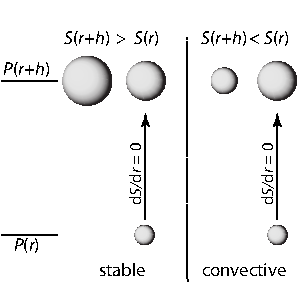
\includegraphics[width=\textwidth]{convective}
\caption[Illustration of criteria for convective instability.]{\label{f.convective-schematic}Illustration of criteria for convective instability.  On the left, raising a blob a distance $h$ adiabatically and in pressure balance with its surrounding results in a higher density $V_{b} < V$.  This is stable: the blob will sink back.  On the right, the blob is less dense and hence buoyant: it will continue to rise.}
\end{marginfigure}

Taking $h$ to be an infinitesimal displacement and expanding the left-hand side of equation~(\ref{e.archimedes}) gives us a local condition for stability:
\begin{equation}\label{e.convective-stability}
V[P(r+h),S(r)] + \tderiv{V}{S}{P}\frac{\dif S}{\dif r} - V[P(r+h),S(r)]  = \tderiv{V}{S}{P}\frac{\dif S}{\dif r} > 0 .
\end{equation}
Noting that
\begin{eqnarray*}
\tderiv{V}{T}{P} &=& \tderiv{V}{S}{P}\tderiv{S}{T}{P}\\
 &=& \frac{C_{P}}{T}\tderiv{V}{S}{P},
 \end{eqnarray*}
 we can rewrite equation~(\ref{e.convective-stability}) as
 \[
 \frac{T}{C_{P}}\tderiv{V}{T}{P}\frac{\dif S}{\dif r} > 0.
 \]
Now, $(\partial V/\partial T)_{P}$ is positive (gas expands on being heated), so our condition for stability is simply
 \begin{equation}\label{e.entropy-condition}
\frac{\dif S}{\dif r} > 0.
\end{equation}
In a convectively stable star, the entropy must increase with radius. if $\dif S/\dif r < 0$, then convection occurs and carries high-entropy material outward, where it will eventually mix with the ambient medium.  As a result, convection drives the entropy gradient toward the marginally stable configuration $\dif S/\dif r = 0$.  If a star is fully convective and mixes efficiently, then the interior of the star lies along an adiabat. 

\section{The adiabatic thermal gradient}\label{s.adiabatic-gradient}

We saw that the temperature gradient in the star is (eq.~[\ref{e.gradient-temperature}])
\[
    \DD{T}{r} = -\frac{3\rho\kappa}{4acT^3}\frac{L(r)}{4\pi r^2}.
\]
Here $\kappa$ is the opacity and $L(r)$ is the luminosity at radius $r$: $L/4\pi r^2$ is the flux. If this thermal gradient, $|\dif T/\dif r|$, becomes too large, however, the fluid becomes unstable: warm fluid begins to rise while cold fluid sinks to take its places.  This usually occurs quickly enough that there is little exchange of heat between the upwelling warm current and the sinking cold one.

As a result of this lack of heat exchange, the motions are termed \newterm{adiabatic}.  To understand what this means, recall the first law of thermodynamics\cite{Fermi1956Thermodynamics}, which relates the change in internal energy $\dif U$ and in volume $\dif V$ to the heat transferred $\dif Q$:
\begin{equation}\label{e.first-law-thermo}
	\dif Q = \dif U + P\dif V,
\end{equation}
where $P$ is the pressure. Now, we aren't using volume to describe our fluid so let's apply this equation to a fixed mass of fluid, say $m = \val{1}{\kilo\gram}$, and divide both sides of Equation~(\ref{e.first-law-thermo-astro}) by the mass. Then $Q$ refers to the heat transferred \emph{per kilogram}, and $U$ refers to the internal energy \emph{per kilogram}.  Instead of $\dif V$, we then have $\dif(V/m) = \dif(1/\rho) = -\rho^{-2}\dif\rho$.  Our first law, rewritten in terms of mass-specific quantities, is thus
\begin{equation}\label{e.first-law-thermo-astro}
	\dif Q = \dif U -\frac{P}{\rho^{2}}\dif \rho.
\end{equation}
Suppose we wish to express quantities in terms of temperature $T$ and density $\rho$: then
\[ \dif U = \tderiv{U}{T}{\rho}\dif T + \tderiv{U}{\rho}{T}\dif \rho, \]
and
\[ \dif Q = \tderiv{U}{T}{\rho}\dif T + \left[\tderiv{U}{\rho}{T} - \frac{P}{\rho^{2}}\right]\dif \rho. \]
Hence the heat needed to raise the temperature of one kilogram of fluid when holding density fixed is
\begin{equation}\label{e.CV}
C_{\rho} \equiv \tderiv{Q}{T}{\rho} = \tderiv{U}{T}{\rho}.
\end{equation}
For an ideal gas, $U = U(T)$ and $C_{\rho}$ is approximately constant; hence we may integrate equation~(\ref{e.CV}) to obtain $U = C_{\rho}T + \textrm{const}$.

In Eq.~(\ref{e.first-law-thermo-astro}), the last term is $-(P/\rho)\, (\dif\rho/\rho) = -(P/\rho)\,\dif\ln\rho$. This demonstrates a useful trick: take the logarithm of the equation of state, $\ln (P) = \ln(\rho) + \ln (T) + \ln (\kB/\mu\mb)$, and then take the differential to obtain
\[ \frac{\dif P}{P} = \frac{\dif\rho}{\rho} + \frac{\dif T}{T}. \]
Now eliminate $\dif\rho/\rho$ in the equation
\[ \dif Q = C_{\rho}\dif T - \frac{P}{\rho}\frac{\dif\rho}{\rho} \]
to obtain an expression for the heat transferred as a function of temperature and pressure,
\[ \dif Q = \left[C_{\rho} + \frac{P}{\rho T}\right]\dif T - \frac{1}{\rho}\dif P
	 = \left[C_{\rho} + \frac{\kB}{\mu\mb}\right]\dif T - \frac{1}{\rho}\dif P. \]
From this we see that the heat needed to raise the temperature of one kilogram when holding pressure fixed is
\begin{equation}\label{e.CP}
C_{P}\equiv \tderiv{Q}{T}{P} = C_{\rho} + \frac{\kB}{\mu\mb}.
\end{equation}
For a plasma of ions and electrons, $C_\rho = (3/2)\kB/(\mu\mb)$ and hence $C_P = (5/2)\kB/(\mu\mb)$.  The ratio of specific heats is
\begin{equation}\label{e.gamma}
    \gamma = \frac{C_P}{C_\rho} = \frac{5/2}{3/2} = \frac{5}{3}.
\end{equation}
This value of $\gamma$ is for an ideal gas and does not hold universally.

\newthought{During adiabatic motion, there is no heat exchange:} hence, the entropy is constant,
\begin{equation}\label{e.differential-entropy}
    T\dif S = \dif Q = 0 = C_{P}\dif T - \frac{1}{\rho} \dif P.
\end{equation}
Using the ideal gas equation of state we can write 
\[
    \frac{1}{\rho} = \frac{\kB}{\mu\mb} \frac{T}{P}
\]
and insert this into Equation~(\ref{e.differential-entropy}) to obtain
\begin{equation}\label{e.differential-adiabat}
     \frac{\dif T}{T} = \frac{\kB/(\mu\mb)}{C_{P}}\frac{\dif P}{P} = \frac{C_{P}-C_{\rho}}{C_{P}} \frac{\dif P}{P} = \frac{\gamma-1}{\gamma}\frac{\dif P}{P}.
\end{equation}
Integrating both sides of the equation gives
\[ \ln T = \frac{\gamma-1}{\gamma}\ln P + \textrm{const.},\]
or 
\begin{equation}\label{e.adiabat}
 T = T_{0}\left(\frac{P}{P_{0}}\right)^{(\gamma-1)/\gamma},
\end{equation}
where $T_{0}$ and $P_{0}$ are the temperature and pressure at the beginning of the adiabatic process.
Equation~(\ref{e.adiabat}) tells us how the temperature changes with pressure along an adiabat for an ideal gas.  Notice that we can recast Equation~(\ref{e.differential-adiabat}) as
\begin{equation}
    \frac{P}{T}\left(\dd{T}{P}\right)_s = \left(\dd{\ln T}{\ln P}\right)_s = \frac{\gamma-1}{\gamma}.
\label{e.nabla-adiabat}
\end{equation}
Equation~(\ref{e.nabla-adiabat}) tells us how temperature changes with pressure in an adiabatically stratified gas.

\newthought{We can derive a condition for convective stability} in terms of the local gradients of temperature and pressure. Writing $S = S[P(r),T(r)]$ we expand equation~(\ref{e.entropy-condition}) to obtain
\begin{equation}\label{e.schwarzschild-1}
\frac{\dif S}{\dif r} = \tderiv{S}{P}{T} \frac{\dif P}{\dif r} + \tderiv{S}{T}{P}\frac{\dif T}{\dif r} .
\end{equation}
Now, $P$ is a monotonically decreasing function of $r$, which means we can change variables:
\begin{equation}\label{e.TPstar}
\frac{\dif T}{\dif r} = \TPstar \frac{\dif P}{\dif r} .
\end{equation}
Here $\dif T/\dif P|_{\star}$ is the slope of the $T(P)$ relation \emph{for the stellar interior}.  In particular, this is \emph{not} a thermodynamic equality. Substituting equation~(\ref{e.TPstar}) into equation~(\ref{e.schwarzschild-1}), using hydrostatic equilibrium to eliminate $\dif P/\dif r$, and recognizing that $(\partial S/\partial T)_{P} = C_{P}/T$, we obtain
\begin{equation}\label{e.schwarzschild-2}
\frac{\dif S}{\dif r} =  -\rho g\left[\tderiv{S}{P}{T} + \frac{C_{P}}{T} \TPstar \right].
\end{equation}
Finally, we can use the identity
\begin{equation}
\tderiv{S}{P}{T}\tderiv{T}{S}{P}\tderiv{P}{T}{S} = -1
\end{equation}
to simplify equation~(\ref{e.schwarzschild-2}),
\begin{equation}
\frac{\dif S}{\dif r} = -\frac{\rho g}{P}C_{P}\left[\frac{P}{T}\TPstar - \frac{P}{T}\tderiv{T}{P}{S}\right].
 \label{e.schwarzschild}
\end{equation}
Hence, if the term in $\left[\cdot\right]$ is positive, then the fluid is convectively unstable.

Let's use our expression for the flux, Equation~(\ref{e.gradient-temperature}), to put $\left.\dif T/\dif P\right|_\star$ in terms of $\kappa$ and $L(r)$:
\begin{eqnarray}
    \frac{P}{T}\TPstar &=& \frac{P}{T}\DD{T}{r}\DD{r}{P} = \frac{P}{\rho g(r)}\frac{1}{\color{red}T}\frac{{\color{red}3}\rho\kappa}{4c {\color{red}a T^3}}\frac{L(r)}{4\pi r^2} \nonumber\\
    &=& \frac{P}{\color{red}\Prad}\frac{\kappa}{16\pi Gc} \frac{L(r)}{m(r)}.
\end{eqnarray}
The fluid is unstable to convection if
\begin{equation}
    \frac{P}{\Prad}\frac{\kappa}{16\pi Gc}\frac{L(r)}{m(r)} > \tderiv{\ln T}{\ln P}{S}  = \frac{\gamma -1}{\gamma}.
\end{equation}
We have used Equation~(\ref{e.nabla-adiabat}) for the last term here.
This occurs for large $\kappa$ (outer layers of cool stars) or for a high $L(r)/m(r)$ (centers of luminous hot stars).  On the main-sequence, stars with $M \lesssim \Msun$ have convective outer layers; stars with $M \lesssim \val{0.3}{\Msun}$ are fully convective. Stars with $M\gtrsim\Msun$ have convective cores.

\begin{marginfigure}
\includegraphics[width=\linewidth]{convection_hinode}
\caption{\label{f.solar-convection]} Solar convection cells, imaged with the Hinode Solar Optical Telescope. Image credit: Hinode JAXA/NASA/PPARC.}
\end{marginfigure}

\begin{exercisebox}[Onset of convection]
The figure shows some hypothetical runs of temperature with respect to pressure in a gas in hydrostatic equilibrium.  Indicate which of these situations is convectively unstable, and explain why. Draw on that plot the pressure-temperature relation that would ensue once convection sets in.

\includegraphics[width=\linewidth]{convection-worksheet-1}
\end{exercisebox}

\begin{exercisebox}[Temperature and density within a star]
The figure below indicates the central density and temperature (\emph{triangle}) for 3 hypothetical stars: (\emph{left}) a star that is fully convective; (\emph{center}) a star with a radiative (i.e., stable against convection) core (densities greater than $\val{10}{\kilo\gram\usk\meter^{-3}}$) and a convective envelope; (\emph{right}) a star with a convective core and a radiative envelope.  For each star, sketch a plausible run of temperature with density within the star. In the center and right panels, the boundary between radiative and convective regions is marked with a vertical solid line.

\includegraphics[width=\linewidth]{convection-worksheet-2}
\end{exercisebox}




\chapter{Burn}\label{ch.nuclear-burning}
% !TEX root = ../intro-stellar-physics.tex

\section{The Coulomb barrier}

Let's take two nuclei with masses\sidenote{When doing kinematics, we shall make the approximation $m\approx A\mb$.} $A_{1}\mb$ and $A_{2}\mb$. This is a two-body problem, so we transform to the center-of-mass frame; the problem reduces to that of one particle, mass $A\mb = A_{1}A_{2}/(A_{1}+A_{2})\times\mb$, moving in a potential.  At distances $\gtrsim \val{2}{\fermi}$, the potential is all Coulomb\sidenote{We write the force between two electrons as $e^2/r^2$.},
\[ \frac{Z_{1}Z_{2}e^{2}}{r} = \val{1.44}{\MeV}\times Z_{1}Z_{2}\left(\frac{\val{1}{\fermi}}{r}\right). \]
We show in Fig.~\ref{f.tunneling} this Coulomb potential as a red curve.
At closer distances the nuclear potential forms a deep well with a repulsive core (blue curve in Fig.~\ref{f.tunneling}).

\begin{figure}[hb]
\includegraphics[width=\linewidth]{Tunneling}
\caption{Tunneling through the Coulomb potential barrier.}
\label{f.tunneling}
\end{figure}

\newthought{Suppose we shoot the particle in from infinity:} How close does the particle come before stopping? For the sun, $E \sim \val{1}{\keV}$ (black line in Fig.~\ref{f.tunneling}).  Equating this energy with the potential and solving for $r$ gives the \emph{turning radius}
\begin{equation}
	r_{E} = \frac{Z_{1}Z_{2}e^{2}}{E} = Z_{1}Z_{2}\times \left(\frac{\val{1}{\keV}}{E}\right) \times \val{1440}{\fermi}.
\end{equation}
This is much bigger than the nuclear radius.  Classically the particle can't go in the region $r<r_{E}$.

The world is quantum, however: the particle wavefunction (thin gray line) decreases exponentially in this region, but there is a finite probability for the particle to reach $r\sim\val{1}{\fermi}$.  This probability is
\[ \mathcal{P}\approx \exp\left[-2\pi^{2}\frac{r_{E}}{\lambda}\right] \]
where $\lambda = h/p$, $p$ being the momentum of the particle.

Expanding,
\[ \frac{2\pi^{2}r_{E}}{\lambda} = 2\pi^{2}\left(\frac{Z_{1}Z_{2}e^{2}}{E}\right)
	\left(\frac{p}{h}\right) = \left[\sqrt{2}\pi \frac{Z_{1}Z_{2}e^{2}}{\hbar}\right]\left(\frac{1}{E}\right)^{1/2}, \]
so we write
\begin{equation}
\mathcal{P} \approx \exp\left[-\left(\frac{\EG}{E}\right)^{1/2}\right],
\end{equation}
with
\[ \EG \equiv \textrm{``Gamow Energy''} = \left[\frac{2\pi^{2}Z_{1}Z_{2}e^{4}m}{\hbar^{2}}\right] = Z_{1}^{2}Z_{2}^{2}A \times \val{979}{\keV}.
\]

\section{The cross-section}
The cross-section for scattering in general is proportional to the ``size'' of the wavefunction, 
\[\sigma\propto \pi\left(\frac{\lambda}{2\pi}\right)^{2} = \pi \left(\frac{\hbar}{p}\right)^{2} = \pi\frac{\hbar^{2}}{2mE}.\]
To get the cross-section for a reaction, we multiply this by the probability of tunneling through the Coulomb barrier, $\mathcal{P} = \exp\left[-\left(\EG/E\right)^{1/2}\right]$, and a term $S(E)$ that accounts for the nuclear interaction.

Putting this all together, we write the reaction cross-section as
\begin{equation}\label{e.s-def}
\sigma(E) = \frac{S(E)}{E}\exp\left[-\left(\frac{\EG}{E}\right)\right].
\end{equation}
It turns out that $S(E)$ is nearly constant\sidenote{This is true as long as we are not close to a resonance---an energy level in the compound nucleus that matches the energy of the incoming particle.}, which helps with extrapolating the cross-section from laboratory energies  to the much lower stellar energies.

\section{The reaction rate}
Recall that the mean-free path of a particle is $\ell = (n\sigma)^{-1}$, where $n$ is the density of targets.  For a particle traveling at speed $v$, the mean time between collisions is therefore $\ell/v$; in a large ensemble of particles, this gives the mean rate, $r = n\sigma v$.  Here $v = |\bvec{v}_{1}-\bvec{v}_{2}|$ is the relative velocity between the particles.  Since the cross-section depends on energy, the rate at which any given particle 1 will react with particles of type 2 having velocities $\bvec{v}_{2}$ in a range $\dif^{3}v_{2}$ is
\[ n_{2} \sigma |\bvec{v}_{1}-\bvec{v}_{2}| \left(\frac{m_{2}}{2\pi kT}\right)^{3/2}\exp\left(-\frac{m_{2}v_{2}^{2}}{2kT}\right) \,\dif^{3}v_{2}. \]
The extra terms are because the particles have a Maxwell-Boltzmann distribution of velocities.  To get the total rate per unit volume, we then have to multiply by the number of particles of type 1 having velocities $\bvec{v}_{1}$ in a range $\dif^{3} v_{1}$ and integrate\sidenote{If particle 1 and particle 2 are identical, for example in the reaction $p+p$, then divide the rate by 2 to avoid double-counting.} over $\dif^{3}v_{1}\,\dif^{3}v_{2}$:
\begin{eqnarray}\label{e.rate-joint}
\lefteqn{r_{12} = n_{1}n_{2}  \left[\frac{m_{1}m_{2}}{(2\pi kT)^{2}}\right]^{3/2}}
  \nonumber\\ &&\times\int\! \sigma(E) v\exp\left(-\frac{m_{1}v_{1}^{2}}{2kT}-\frac{m_{2}v_{2}^{2}}{2kT}\right)  \,\dif^{3} v_{1}\,\dif^{3}v_{2}.
\end{eqnarray}
Now $E$ and $v$ are the relative energies and velocity in the center-of-mass frame.  We can change variable using the relations
\begin{eqnarray*}
\bvec{v}_{1} &=& \bvec{V} - \frac{m_{2}}{m_{1}+m_{2}} \bvec{v}\\
\bvec{v}_{2} &=& \bvec{V} + \frac{m_{1}}{m_{1}+m_{2}} \bvec{v}.
\end{eqnarray*}
where $V$ is the center-of-mass velocity. It is straightforward to show that $\dif v_{1,x}\,\dif v_{2,x} = \dif V_{x}\dif v_{x}$, and likewise for the $y,z$ directions.  Furthermore, $m_{1}v_{1}^{2} + m_{2}v_{2}^{2} = (m_{1}+m_{2})V^{2} + m v^{2}$, and multiplying and dividing the integral in equation~(\ref{e.rate-joint}) by $m_{1}+m_{2}$ allows us to write
\begin{eqnarray*}
\lefteqn{r_{12} = n_{1}n_{2} \left(\frac{m_{1}+m_{2}}{2kT}\right)^{3/2}\left(\frac{m}{2kT}\right)^{3/2}}\\
&&\times \int\!\dif^{3}V \int\!\dif^{3}v \,\sigma(E)v \exp\left[-\frac{mv^{2}}{2kT}\right]
 \exp\left[-\frac{(m_{1}+m_{2})V^{2}}{2kT}\right].
\end{eqnarray*}
The integral over $\dif^{3}V$ can be factored out and is normalized to unity. Hence we have for the reaction rate between a pair of particles 1 and 2, 
\begin{eqnarray}\label{e.rate}
r_{12} &=& n_{1}n_{2}\left\{\left(\frac{m}{2\pi kT}\right)^{3/2}\int_{0}^{\infty}\! \sigma(E) v \exp\left(-\frac{mv^{2}}{2kT}\right)  4\pi v^{2}\,\dif v\right\}.\nonumber\\
 &\equiv& \frac{1}{1+\delta_{12}}n_{1}n_{2}\langle\sigma v\rangle.
\end{eqnarray}
The term in $\{\}$ is the averaging over the joint distribution of the cross-section times the velocity, and is usually denoted as $\langle\sigma v\rangle$. 

Changing variables to $E = mv^{2}/2$ in equation~(\ref{e.rate}) and inserting the formula for the cross-section, equation~(\ref{e.s-def}), gives
\begin{equation}\label{e.integral}
\langle\sigma v\rangle = \left(\frac{8}{\pi m}\right)^{1/2}\left(\frac{1}{kT}\right)^{3/2}\int_{0}^{\infty}\!S(E)\exp\left[-\left(\frac{\EG}{E}\right)^{1/2}-\frac{E}{kT}\right]\,\dif E.
\end{equation}
Now, we've assumed that $S(E)$ varies slowly; but look at the argument of the exponential. This is a competition between a rapidly rising term $\exp[-(\EG/E)^{1/2}]$ and a rapidly falling term $\exp(-E/kT)$. As a result, the exponential will have a strong peak, and we can expand the integrand in a Taylor series about the maximum. Let 
\[
f(E) = -\left(\frac{\EG}{E}\right)^{1/2} - \frac{E}{kT}.
\]
Then we can write 
\begin{eqnarray*}
\lefteqn{\int_{0}^{\infty}\!S(E)\exp\left[-\left(\frac{\EG}{E}\right)^{1/2}-\frac{E}{kT}\right]\,\dif E}\\
&\approx&
	\int_{0}^{\infty}\! S(\Epk)\exp\left[f(\Epk) + \frac{1}{2}\left.\frac{\dif^{2} f}{\dif E^{2}}\right|_{E=\Epk}\left(E-\Epk\right)^{2}\right].
\end{eqnarray*}
Here $\Epk$ is found by solving $(\dif f/\dif E)|_{E=\Epk} = 0$. This trick allows us to turn the integral into a Gaussian! (Before the internet, all there was to do for fun were integrals.)

Solving for \Epk, we get
\[
\Epk = \frac{\EG^{1/3}(kT)^{2/3}}{2^{2/3}},
\]
and 
\[ \exp\left[f(\Epk)\right] = \exp\left[-3\left(\frac{\EG}{4kT}\right)^{1/3}\right].
\]
Further,
\[
\left.\frac{1}{2}\frac{\dif^{2}f}{\dif E^{2}}\right|_{E=\Epk} = -\frac{3}{2(2\EG)^{1/3}(kT)^{5/3}} = -\frac{3}{4\Epk kT}.
\]
Defining a variable $\Delta = 4(\Epk kT/3)^{1/2}$, our integral becomes
\begin{eqnarray}\label{e.integral2}
\lefteqn{\langle\sigma v\rangle = \left(\frac{8}{\pi m}\right)^{1/2}\left(\frac{1}{kT}\right)^{3/2}}\nonumber\\
&&\times S(\Epk)
  \exp\left[-3\left(\frac{\EG}{4kT}\right)^{1/3}\right]
  \int_{0}^{\infty}\!\exp\left[-\frac{(E-\Epk)^{2}}{(\Delta/2)^{2}}\right]\,\dif E.
\end{eqnarray}
How well does this approximation do?  Figure~\ref{f.integrand} shows the integrand (\emph{solid line}) and the approximation by a Gaussian (\emph{dashed line}).  Although the integrand is skewed to the right, the area is approximately the same.  
\begin{marginfigure}
\includegraphics[width=\linewidth]{coulomb_integrand}
\caption[Terms in integrand for calculating Coulomb barrier]{Integrand of eq.~(\protect\ref{e.integral}) (\emph{solid line}) and the Gaussian (\emph{dot-dashed line}) constructed by expanding to second order the argument of the exponential. The parameters for $\EG$ were taken from the $p+p$ reactions ($Z_{1}Z_{2}=1$, $A = 1/2$), and the temperature is $\val{10^{7}}{\K}$.  Note that the grey curves, showing the two terms of the exponential, have been rescaled to fit on the same plot.}
\label{f.integrand}
\end{marginfigure}

Another simplification can be made because both the Gaussian and the original integrand go to zero as $E\to 0$.  As a result, we can extend the lower bound of our integral (eq.~[\ref{e.integral2}]) to $-\infty$, and obtain
\begin{eqnarray}\label{e.rate2}
\langle\sigma v\rangle &\approx& \left(\frac{8}{\pi m}\right)^{1/2}\left(\frac{1}{kT}\right)^{3/2} S(\Epk) \exp\left[-3\left(\frac{\EG}{4kT}\right)^{1/3}\right]\frac{\Delta}{2}\nonumber\\
 &=& \frac{2^{13/6}}{\sqrt{3m}}\frac{\EG^{1/6}}{(kT)^{2/3}} \exp\left[-3\left(\frac{\EG}{4kT}\right)^{1/3}\right]  S(\Epk).
\end{eqnarray}
On to some numbers. Table~\ref{t.reaction} lists quantities for some common reactions. A couple of notes. First, $\Delta/\Epk$ indicates how well our Gaussian approximation works---you will see it is less than 1 in all cases. We evaluated $\Delta/\Epk$, which decreases with temperature as $T^{-1/6}$, at $T = \val{10^{7}}{\K}$. Second, the quantity $n(T)$ is the exponent if we want to approximate the reaction rate as a power-law, $r\propto T^{n}$.  We compute this as 
\begin{equation}\label{e.exponent}
 n(T) = \dd{\ln r}{\ln T} = -\frac{2}{3} + \left(\frac{\EG}{4kT}\right)^{1/3},
\end{equation}
as you can verify for yourself. In the table, the exponent is evaluated at $T = \val{10^{7}}{\K}$; the exponent $n$ depends on temperature. Finally, note the size of $\EG/(4k)$.  This makes the argument of the exponential in equation~(\ref{e.rate2}) large in absolute value, and sets the temperature scale at which a given reaction comes into play.
 
\begin{table}[hb]
\caption{\label{t.reaction} Parameters for non-resonant reactions}
\begin{center}
\begin{tabular}{lrrrrrr}
\hline
Reaction & $p+p$ & $p+\helium[3]$ & $\helium[3]+\helium[3]$ & $p+\lithium[7]$ & $p+\carbon$\\
\hline\hline
$A$ & 1/2 & 3/4 & 3/2 & 0.88 & 0.92 \\
$Z_{1}Z_{2}$ & 1 & 2 & 4 & 3 & 6 \\
$\EG$ (MeV) & 0.489 & $2.94$ & $23.5$ & $7.70$ & $32.5$\\
$\EG/(4k)$ (GK) & $1.4$ & $8.5$ & $68.0$ & $22.0$ & $94.0$ \\
$\Epk|_{T=\val{10^{7}}{\K}}$ (keV) & 4.5 & 8.2 & 16.3 & 11.3 & 18.2\\
$\Delta/\Epk|_{T=\val{10^{7}}{\K}}$ & 1.0 & 0.75 & 0.53 & 0.64 & 0.50 \\
$n(T = \val{10^{7}}{\K})$ & 4.6 & 8.8 & 18.3 & 12.4 & 20.5\\
\hline
\end{tabular}
\end{center}
\end{table}


\chapter{Star}\label{ch.main-sequence}
% !TEX root = ../intro-stellar-physics.tex

We now have almost all of the physics necessary to describe the lift of a star. The nuclear physics enters in an equation for the luminosity, which we shall derive next. We then need to discuss departures from the classical ideal gas equation of state; this becomes important for low-mass stars and sets the minimum stellar mass.

\section{The luminosity equation}

We've established the relations for the enclosed mass,
\begin{equation}\label{e.mass}
\DD{m}{r} = 4\pi r^{2}\rho,
\end{equation}
the pressure,
\begin{equation}\label{e.pressure}
\DD{P}{r} = -\rho\frac{Gm}{r^{2}},
\end{equation}
and the temperature,
\begin{eqnarray}\label{e.temperature-radiative}
\DD{T}{r} &=& - \frac{L}{4\pi r^{2}}\frac{3\rho\kappa}{4ac T^{3}}\qquad \textrm{in radiative regions;} \\ 
\label{e.temperature-convective}
\DD{T}{r} &=& \frac{T}{P}\tderiv{\ln T}{\ln P}{S}\DD{P}{r} \quad \textrm{in convective regions}.
\end{eqnarray}
We need an equation for the luminosity $L(r)$, which we now derive.

\begin{marginfigure}
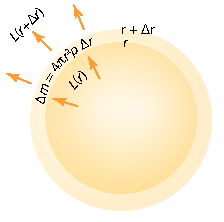
\includegraphics[width=\linewidth]{luminosity-eqn}
\caption[Heat balance in a mass shell]{Heat balance in a shell $\Delta m$.}
\label{f.luminosity}
\end{marginfigure}
Suppose we have a shell of mass $\Delta m$ lying between surfaces $r$ and $r+\Delta r$ (Fig.~\ref{f.luminosity}). The shell gains heat from nuclear reactions at a rate $\Delta m \times \varepsilon$, where $\varepsilon$ is the heating rate per unit mass.  In addition, there is heat entering the shell from below at a rate $L(r)$ and heat leaving the top of the shell at a rate $-L(r+\Delta r)$.
If the shell is neither gaining or losing heat, then these terms must balance:
\[ 4\pi r^{2}\rho\varepsilon\,\Delta r + L(r) - L(r+\Delta r) = 0. \]
This reduces to our fourth equation of stellar structure,
\begin{equation}
\label{e.luminosity}
\DD{L}{r} = 4\pi r^{2}\rho\varepsilon.
\end{equation}
These equations are supplemented by an equation of state $P = P(\rho,T)$.

\section{Contraction to the main sequence}
\label{s.contraction-to-main-sequence}
When the core is too cool for nuclear reactions to power the luminosity from the surface (remember, the luminosity is set by the mass of the star and its opacity) then the star must contract.\marginnote{When the radius is changing, an extra term appears in eq.~(\ref{e.luminosity}) giving the luminosity evolved from gravitational contraction.}

\subsection{Degeneracy}
\label{s.degeneracy}

As a star contracts, the particles within it are packed ever closer together.  As we saw from our discussion of ionization, the behavior of particles must change when the separation between particles is of the order of the uncertainty in their positions.  Equivalently, our classical description breaks down when the particle density exceeds roughly
\begin{equation}\label{e.heuristic-quantum-density}
    \frac{1\;\textrm{particle}}{(\Delta x)^3} 
    = \left(\frac{\Delta p}{h}\right)^3 
    \sim \left(\frac{m\kB T}{h^2}\right)^{3/2}.
\end{equation}
Another way to put this is that quantum effects become important when there is roughly 1 particle in a normalized phase space volume $\dif^{3}x\,\dif^{3}p/h^{3}$.

Suppose we have two identical particles in a quantum state. Since the particles are identical, if we exchange them the wavefunction can only change by a phase factor\sidenote{See Box~\ref{sb.identical-particles}} $e^{i\delta}$. If we exchange the particles again, we are back to our original state; as a result, $e^{2i\delta} = 1$, and therefore $\delta = 0$ or $\pi$. Hence upon the exchange of particles, the wavefunction either is unchanged ($\delta=0$) or it changes sign ($e^{i\pi}=-1$).
\begin{quote}\itshape
    There are two types of particles in this world: those that change sign under exchange; and those that don't.
\end{quote}
Particles that don't change sign under exchange are called \newterm{bosons} and have integer spin. Photons are bosons. Particles that change sign under exchange are called \newterm{fermions} and have half-integer spin. Electrons, neutrinos, protons, and neutrons are all fermions. 

A consequence of the fermion wavefunction changing sign when any two particles are exchanged is that the wavefunction vanishes if any two particles are in the same state---that is, they have the same position, momentum, and spin. For spin-half particles like electrons, then means we can put at most two such electrons in the same position and momentum state; we do this by having their spins antiparallel.

\begin{sidebar}[Identical Particles]
\label{sb.identical-particles}
To understand how the interchange of identical particles works in more detail, let's start by recalling some features of quantum mechanics. This discussion is based on the treatment of \citet{Feynman1989The-Feynman-Lec}.
We denote a state as $\ket{a}$, where $a$ is just a label.  For example, $a$ could be "electron with such-and-such momentum".  The probability of finding the electron in some other state $\phi$ is given by $|\braket{\phi}{a}|^2$, where $\braket{\phi}{a}$ is a complex number known as the probability amplitude.

Now suppose we have two particles, a and b, and we scatter them so that one particle ends up in detector 1 and the other ends up in detector 2. There are two ways this can go, as shown here.
\begin{center}
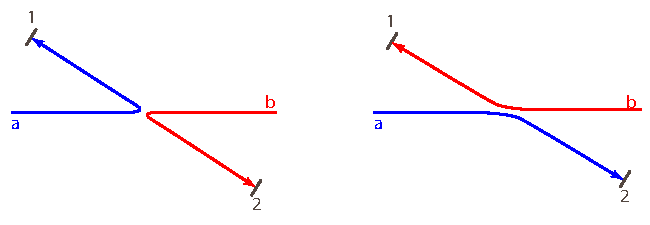
\includegraphics[width=\linewidth]{scattering-classical}
\end{center}
Classically, we would argue that the probability of getting either particle in detector 1 is just
\begin{equation}
    \mathcal{P}(\textrm{a or b in 1}) = \mathcal{P}(\textrm{a in 1}) + \mathcal{P}(\textrm{b in 1}).
\end{equation}
If particles a and b are different---e.g., one is a \carbon\ nucleus and the other is an \oxygen\ nucleus---then this holds in quantum mechanics as well. Quantum mechanically, we write
\begin{equation}
    \mathcal{P}(\textrm{a or b in 1}) = |\braket{1}{a}\braket{2}{b}|^2 + |\braket{2}{a}\braket{1}{b}|^2.
\end{equation}
If the particles are identical, however---for example, if a and b are two electrons with identical spin---then this picture is wrong.

Because of the uncertainty principle, we cannot follow the trajectories of a and b with infinite precision to see which is which; instead, the situation is more analogous to the depiction shown here.
\begin{center}
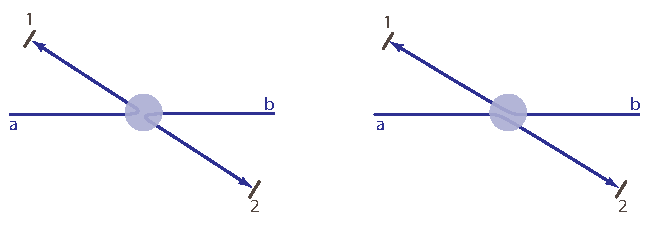
\includegraphics[width=\linewidth]{scattering-quantum}
\end{center}
There are now two indistinguishable ways of arriving at the final state---in this case, an electron in detector 1 and an electron in detector 2. According to quantum mechanics, we must therefore sum the amplitudes for getting to the final state, \emph{before taking the square}. That is, the probability for this one particle to end up in detector 1 and the other to end up in detector 2 is
\begin{eqnarray}
    \mathcal{P}(\textrm{a or b in 1}) &=& |\braket{1}{a}\braket{2}{b} + \braket{2}{a}\braket{1}{b}|^2\nonumber\\
    &=& |\braket{1}{a}\braket{2}{b}|^2 + |\braket{2}{a}\braket{1}{b}|^2 \nonumber\\
    && + {\color{red}\left[ \braket{1}{a}^*\braket{2}{b}^*\braket{2}{a}\braket{1}{b}\right.} \nonumber\\
    && {\color{red}+ \left.\braket{2}{a}^*\braket{1}{b}^*\braket{1}{a}\braket{2}{b}\right]} \nonumber\\
    &=& \mathcal{P}(\textrm{a in 1}) + \mathcal{P}(\textrm{b in 1}) \nonumber\\
    && + {\color{red}\left[ \braket{1}{a}^*\braket{2}{b}^*\braket{2}{a}\braket{1}{b}\right.}\nonumber\\
    && {\color{red}+ \left.\braket{2}{a}^*\braket{1}{b}^*\braket{1}{a}\braket{2}{b}\right]}.
    \label{e.scattering-quantum}
\end{eqnarray}
The probability of scattering an electron into detector 1 is the classical value plus the \emph{additional} interference term in $\color{red}[\cdot]$.

\newthought{To see the effect on the thermal properties,} let's imagine putting two particles into the same small volume.  To do this, we imagine the detectors 1 and 2 sliding together until they overlap, as shown here.  
\begin{center}
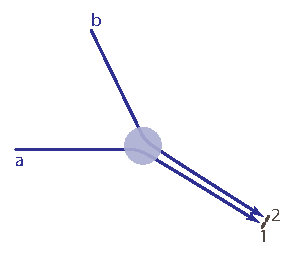
\includegraphics{fermions}
\end{center}
Since detectors 1 and 2 are approaching one another, we must have that
\begin{equation}
    |\braket{1}{a}\braket{2}{b}|^2 = |\braket{2}{a}\braket{1}{b}|^2.
\end{equation}
This does not imply, however, that $\braket{1}{a}\braket{2}{b} = \braket{2}{a}\braket{1}{b}$: the amplitudes could differ by a phase factor, so that interchanging the particles would yield
\[
    \braket{2}{a}\braket{1}{b} = e^{i\delta}\braket{1}{a}\braket{2}{b}.
\]
If we interchange the particles, and then interchange them again, we get
\[
    \braket{1}{a}\braket{2}{b} = e^{2i\delta}\braket{1}{a}\braket{2}{b};
\]
since swapping the particles twice just gets up back to the original situation, we must have that $e^{2i\delta} = 1$ and therefore $e^{i\delta} = \pm 1$.

If there is no change of sign, i.e., $\braket{2}{a}\braket{1}{b} = \braket{1}{a}\braket{2}{b}$, then from equation~(\ref{e.scattering-quantum}) we have
\begin{equation}\label{e.boson}
    \mathcal{P}(\textrm{a or b in 1}) = 2|\braket{1}{a}\braket{2}{b}|^2 + 2|\braket{2}{a}\braket{1}{b}|^2.
\end{equation}
This is \emph{twice} the classical value: the probability of the particles entering the same state is enhanced.

In contrast, if $\braket{2}{a}\braket{1}{b} = -\braket{1}{a}\braket{2}{b}$, then equation~(\ref{e.scattering-quantum}) implies that
\begin{eqnarray}
\mathcal{P}(\textrm{a or b in 1}) &=& |\braket{1}{a}\braket{2}{b}| + |\braket{2}{a}\braket{1}{b}| \nonumber\\ 
    && - |\braket{1}{a}\braket{2}{b}| - |\braket{2}{a}\braket{1}{b}| \nonumber\\ 
    &=& 0.\label{e.fermion}
\end{eqnarray}
\begin{quote}\itshape
We cannot have 2 identical particles with the same momentum, position, and spin if their wavefunction changes sign when the particles are exchanged.
\end{quote}
Particles with integer spin (i.e., their angular momentum is an integer multiple of $\hbar$) have wavefunctions that do not change sign under exchange; these particles are said to obey \emph{Bose-Einstein statistics} and are called \emph{bosons}.  Particles with half-integer spin have wavefunctions that do change sign under exchange; these particles are said to obey \emph{Fermi-Dirac statistics} and are called \emph{fermions}.  Photons are bosons; electrons, protons, neutrons, and neutrinos are fermions.
\end{sidebar}

\newthought{To connect with the equation of state,} we begin by imagining a small volume containing $N$ electrons. Motivated by eq.~(\ref{e.heuristic-quantum-density}), we divide the phase space into cells,
\[
	\frac{\dif^{3}x\,\dif^{3}p}{h^{3}},
\]
and into each cell we place 2 electrons with opposing spins. We always add the electrons to the lowest open energy level, and repeat the process until we have added all $N$ electrons. This procedure is represented by the equation
\begin{equation}
	N = \frac{2}{h^{3}}\int_{V}\dif^{3}x\int_{0}^{\EF}\dif^{3}p
\end{equation}
In this equation $\EF$, the \emph{Fermi energy}, is the energy of the last electrons added and is the largest filled energy level.

If our volume is isotropic, then we can change variables: first, to spherical momentum coordinates, $\dif^{3}p = 4\pi p^{2}\,\dif p$; second, from $\dif p$ to $\dif\varepsilon$.  Since $p = \sqrt{2m\varepsilon}$, where $\varepsilon$ is the energy of a single electron,
\[
	\dif p = \sqrt{\frac{m}{2\varepsilon}}\,\dif \varepsilon;
\]
we can therefore change variables and integrate over $\varepsilon$ from $0$ to $\EF$ to obtain
\[
	N = \frac{8\pi}{h^{3}}V \int_{0}^{\EF} \sqrt{2}m^{3/2}\varepsilon^{1/2}\,\dif \varepsilon
	= \frac{8\pi}{3h^{3}} V (2m)^{3/2} \EF^{3/2}.
\]
Solving for the Fermi energy gives
\begin{equation}\label{e.fermi-energy}
	\EF = \frac{h^{2}}{2m}\left(\frac{3}{8\pi}\frac{N}{V}\right)^{2/3}.
\end{equation}
What is the total energy of our system? We again integrate over phase space, with each electron multiplied by its energy $\varepsilon$:
\begin{equation}\label{e.total-energy}
	E = \frac{8\pi}{h^{3}}V\int_{0}^{\EF}\sqrt{2}m^{3/2}\varepsilon^{3/2}\,\dif\varepsilon = \frac{8\pi}{5h^{3}}V(2m)^{3/2} \EF^{5/2}.
\end{equation}
Using eq.~(\ref{e.fermi-energy}) to substitute for $\EF$ in eq.~(\ref{e.total-energy}), we can find the energy per unit volume,
\[
	\frac{E}{V} = \frac{3}{5}\left(\frac{3}{8\pi}\right)^{2/3}\frac{h^{2}}{2m}n^{5/3} = \frac{3}{5} n \EF,
\]
where $n=N/V$ is the density of electrons.

Recall that for a non-relativistic gas the pressure is $P = (2/3)(E/V)$.  Hence the pressure of our electron gas is
\begin{equation}\label{e.pressure-electrons}
	P = \frac{2}{3}\frac{E}{V} = \frac{2}{5} n\EF
		= \frac{2}{5}\left(\frac{3}{8\pi}\right)^{2/3}\frac{h^{2}}{2m}n^{5/3}.
\end{equation}
Notice that the pressure is independent of the temperature.

The electrons, being more than 1000 times lighter than the nuclei, become degenerate first. Suppose our composition consists of species with charge $Z_{i}$ and mass number $A_{i}$. Then the number of electrons per unit volume\marginnote{assuming complete ionizaton} is
\[
	n_{e} = \sum_{i} n_{i} Z_{i} = \frac{\rho}{\mb}\sum_{i} X_{i}\frac{Z_{i}}{A_{i}}.
\]
By analogy with the mean molecular weight, we define an electron mean weight
\begin{equation}\label{e.electron-mean-weight}
\mu_{e} \equiv \left(\sum_{i}X_{i}\frac{Z_{i}}{A_{i}}\right)^{-1}
\end{equation}
so that $n_{e} = \rho/(\mb\mu_{e})$.

\begin{exercisebox}[The mass-radius relation for a degenerate EOS]
\label{ex.degenerate-mass-radius}
Use equation~(\ref{e.electron-mean-weight}) in eq.~(\ref{e.pressure-electrons}) to express the pressure as a function of mass density $\rho$. The use the virial scalings for $P(M,R)$ and $\rho(M,R)$ to obtain a relation $R(M)$ for a degenerate object. \emph{Hint:} this may be easier to do in a Jupyter notebook.
\end{exercisebox}

As you found in exercise~\ref{ex.degenerate-mass-radius}, when the star becomes degenerate, there is a unique radius for a given mass and composition. This is in contrast to the non-degenerate case, for which a star of a given mass can have a wide range of possible radii depending on the internal temperature.

\section{Summary}

This convective zone changes the structure of the star, so that $L\sim M^{3.5}$ rather than the $M^{3}$ scaling we derived earlier.  It also means the star can burn more of the hydrogen in its interior.  The hotter $\Teff$ means, however, that the opacity is less strong in the surface layers of upper main sequence stars, and so the outer layers are radiative.  Table~\ref{t.MS-characteristics} gives a summary of the properties of main sequence stars.
\begin{margintable}[-6\baselineskip]
\caption{\label{t.MS-characteristics} Characteristics of main-sequence stars}
\centering
\begin{tabular}{lll}
characteristic & $M\lesssim\Msun$ & $M\gtrsim\Msun$\\
\hline
hydrogen burning & pp & CNO\\
core & radiative  & convective\\
envelope & convective & radiative\\
\end{tabular}
\end{margintable}


\chapter{The Equation of State}\label{ch.degeneracy}
\input{degeneracy/degeneracy}

\chapter{End of the Line}\label{ch.post-main-sequence}
% !TEX root = ../intro-stellar-physics.tex

\section{Low-mass stars}
For stars with main-sequence masses $\lesssim \valrng[--]{8}{10}{\Msun}$, the core becomes degenerate before the onset of $\carbon$ fusion.  Indeed, for stars around a solar mass, the fusion of \helium\ occurs under moderately degenerate conditions.

\subsection{Ascent of the red-giant branch}
With the depletion of hydrogen, the core contracts while there is \hydrogen\ fusion occurring in a shell surrounding the core.  The rising temperature and pressure in the shell causes the \hydrogen\ fusion reactions to go at an ever increasing rate.  The high luminosity drives the envelope, now fully convective, to large radii and hence to a low surface temperature. Observationally, the star becomes a red giant.  During this phase the high luminosity, combined with the low surface gravity of the distended envelope, drives a strong wind\sidenote{The exact rate of mass loss is still not well constrained.}.

\subsection{The helium flash}
There are no stable isotopes with mass $A=5$ or $A=8$, which makes the fusion of \helium\ somewhat tricky.  The isotope \beryllium[8] is, however, long-lived ($\val{10^{-16}}{\second}$) compared to a nuclear timescale\sidenote{Roughly the time for a pion to cross a nucleus, $\sim \val{10^{-22}}{\second}$.}.
When the core temperature reaches $\approx\val{10^{8}}{\K}$, the reaction
\[ \helium + \helium \longleftrightarrow\beryllium[8] \]
builds up a small abundance of \beryllium[8]; the reaction
\[ \beryllium[8] + \helium \longleftrightarrow \carbon^{*} \]
then builds up a small abundance of \carbon\ in an excited state (denoted by the $^{*}$).  While the dominant decay channel of $\carbon^{*}$ is $\carbon^{*}\to\beryllium[8]+\helium$, there is a branching to the ground state, $\carbon^{*}\to\carbon+\gamma$; as a result, there is a net conversion $3\helium\to\carbon$---the ``triple-alpha'' reaction.  This reaction is \emph{very temperature-sensitive}: $\partial\ln\epsilon_{3\alpha}/\partial\ln T \approx 40$ at $T = \val{10^{8}}{\K}$; this sensitivity, combined with the mildly degenerate conditions of the core, makes the ignition of \helium\ unstable for solar-mass stars.

\subsection{Helium burning: the horizontal branch}

Once core \helium\ has ignited, the star settles onto a ``Helium Main Sequence;'' observationally this is the \newterm{horizontal branch}, so called because these stars form a noticeable clump on a Hertzsprung-Russell diagram.  The luminosity on the horizontal branch is about \valrng[--]{30}{100}{\Lsun}.  The higher luminosity, combined with the much lower energy release from the $3\helium\to\carbon$, makes the horizontal branch lifetime much shorter than that of the main-sequence (e.g., the horizontal branch lifetime is $\sim \val{10^{8}}{\yr}$ for a solar-mass star.

\subsection{The asymptotic giant branch and planetary nebula}

With the depletion of \helium\ in the core, the core---now composed of \carbon\ and \oxygen---contracts, while the growing luminosity from the H- and He-burning shells again drive the envelope to large radii.  The H- and He-burning shells are often thermally unstable and \emph{pulse}.  The hydrogen-rich envelope is consumed at its base by the H- and He-burning shells and is expelled at the surface by an increasingly strong wind.  After the envelope is gone, the hot core---now called a \newterm{white dwarf}---slowly cools.

\section{Massive stars}

For stars with main-sequence masses $\gtrsim \valrng[--]{8}{10}{\Msun}$, the fusion of \carbon\ commences while the core is non-degenerate.  The temperature required is $\approx\val{\sci{8}{8}}{\K}$.  At this temperature, electron-positron pairs can form and annihilate; while this usually produces photons, there is a branch
\[ e^{-}+e^{+} \longleftrightarrow \nu_{e} + \bar{\nu}_{e}\]
that generates a neutrino-antineutrino pair. The mean free path for the neutrinos is larger than the radius of the star; as a result, this process efficiently cools the core.

After this point, the core evolves on a timescale that is too fast for the envelope to keep up.  The fusion of \carbon\ produces $\sodium+\pt$ and $\neon+\helium$; the \pt\ and \helium\ capture onto other nuclei that are present.  At slightly higher temperatures, the reaction $\neon+\gamma \to \oxygen+\helium$ occurs; the \helium\ capture onto other \oxygen, \neon, and \magnesium.

The next significant burning stage is $\oxygen+\oxygen$, which produces $\phosphorus[31]+\pt$ and $\silicon+\helium$; as before, the \pt\ and \helium\ combine with other nuclei and produce a group of nuclei around \silicon.

The strong Coulomb barrier inhibits the fusion of nuclei beyond \oxygen; instead, photodissociation reactions such as $\silicon+\gamma \to \magnesium+\helium$ liberate \nt, \pt, and \helium.  These light nuclei then fuse with other heavy nuclei, and the composition gradually becomes composed of nuclei around \iron.  This is \emph{nuclear statistical equilibrium}: the composition is in the lowest energy state (most bound) for the ambient density and temperature.

\begin{exercisebox}[Dynamical time of evolved stellar core]
At the onset of \oxygen\ burning in a \val{20}{\Msun} star, the central density is $\approx \val{10^{6}}{\grampercc}$.  What is the dynamical time of the core?
\end{exercisebox}

\subsection{A relativistic degenerate equation of state}

For degenerate electrons, the momentum---and hence the kinetic energy---increases with density.  When the kinetic energy approaches the rest mass of the electrons, the relation between kinetic energy and momentum is no longer $E = p^{2}/2m$.  When the electrons are extremely relativistic, their energy becomes $E = p c$.

Recall that for an ideal gas (no interactions) the density of electrons is given by the integral over phase space,
\[
  n = \frac{2}{h^{3}} \int \dif^{3}p \frac{1}{\exp\left[\left(E-\mu\right)/kT\right]+1}.
\]
The $2$ in the numerator is because electrons are spin-$1/2$ particles and there are thus 2 states in the same infinitesimal $\dif^{3}p$.  If the electrons are degenerate, $kT \ll E,\mu$ and the integral becomes
\[
  n = \frac{2}{h^{3}}\int_{0}^{E_{F}} \dif^{3}p = \frac{8\pi}{h^{3}} \int_{0}^{E_{F}} p^{2}\,\dif p = \frac{8\pi}{h^{3}c^{3}} \int_{0}^{E_{F}} E^{2}\,\dif E = \frac{8\pi}{3h^{3}c^{3}} E_{F}^{3}.
\]
Hence the electrons are characterized by a Fermi energy
\begin{equation}\label{e.fermi}
	E_{F} = \left(\frac{3}{8\pi}\right)^{1/3}hc\; n^{1/3}
\end{equation}
With this we can find the energy density
\[
  U = \frac{8\pi}{h^{3}c^{3}}\int_{0}^{E_{F}} E^{3}\,\dif E = \frac{3}{4} n E_{F};
\]
and for a relativistic gas the pressure is $U/3$, or
\begin{equation}\label{e.pressure-relativistic}
  P = \frac{1}{4}n E_{F} = \frac{1}{4}\left(\frac{3}{8\pi}\right)^{1/3}hc\; n^{4/3}.
\end{equation}
Here $n = \rho/(\mb\mu_{e})$ is the number of electrons per unit volume.

\subsection{The Chandrasekhar mass}
We constructed a mass-radius relation for white dwarfs by combining the virial relations,
\begin{eqnarray*}
   P    &\propto& \frac{GM^{2}}{R^{4}}\\
   \rho &\propto& \frac{M}{R^{3}}
\end{eqnarray*}
and the equation of state for a non-relativistic, degenerate, ideal gas.  We found that $R\propto M^{-1/3}$.  If we try that with our relativistic equation of state, eq.~(\ref{e.pressure-relativistic}), we get
\[
	\frac{GM^{2}}{R^{4}} \propto P = \frac{1}{4}\left(\frac{3}{8\pi}\right)^{1/3}hc\; \left(\frac{\rho}{\mb\mu_{e}}\right)^{4/3} \propto \left(\frac{M}{R^{3}}\right)^{4/3}.
\]
The radius $R$ cancels, and what we have is a relation $M\propto (hc/G)^{3/2}/\mb^{2}$.  This is rather odd: hydrostatic balance and our equation of state produce a characteristic mass in terms of fundamental constants.

Let's investigate this a bit more.  Suppose we construct a box filled with $N$ electrons and a mass $\mu_{e}\mb N$.  The volume of the box $V \sim R^{3}$, and since the electrons are degenerate, the volume per electron is roughly $\lambda^{3}$, where $\lambda \sim h/p$ is the wavelength of the electrons.  As a result, $N = (R/\lambda)^{3}$; further, the momentum of an electron is
\[	p \sim \frac{h}{\lambda} \sim h\frac{N^{1/3}}{R}. \]
If our electrons were non-relativistic, the total, kinetic plus gravitational, energy of our box would be
\[
	E_{\mathrm{total}} = N\frac{p^{2}}{2m_{e}} - \frac{GM^{2}}{R} \sim N^{5/3}\frac{h^{2}}{R^{2}m_{e}} - GN^{2}\mu_{e}^{2}\mb^{2} \frac{1}{R}.
\]
For a given $N$, we can adjust $R$ to make $E_{\mathrm{total}}<0$, and indeed, if we satisfy the virial theorem, we will recover the $R\propto M^{-1/3}$ scaling.

If, however, the electrons are relativistic then the total energy is
\begin{eqnarray*}
	E_{\mathrm{total}} = Npc - \frac{GM^{2}}{R} 
		&=& \frac{1}{R}\left[hc N^{4/3} - G N^{2}(\mu_{e}\mb)^{2}\right]\\
		&=& G(\mu_{e}\mb)^{2}\frac{N^{4/3}}{R}\left[ {\color{red}\frac{hc}{G(\mu_{e}\mb)^{2}} - N^{2/3}}\right].
\end{eqnarray*}
If $N < [hc/G/(\mu_{e}\mb)^{2}]^{3/2}$, then $E_{\mathrm{total}} > 0$; by making $R$ larger, however, we can lower the energy until the electrons are no longer relativistic.  If $N > [hc/G(\mu_{e}\mb)^{2}]^{3/2}$, then $E_{\mathrm{total}} < 0$; by making $R$ smaller, however, we can keep reducing $E_{\mathrm{total}}$.  There is no bound state with finite $R$.

Thus, there is a limit to the number of degenerate electrons, and hence the total mass, that we can put in hydrostatic equilibrium.  An exact calculation yields
\begin{equation}\label{e.Chandrasekhar}
	M_{\mathrm{Ch}} = 1.456 \left(\frac{2}{\mu_{e}}\right)^{2}\Msun.
\end{equation}
When the mass reaches this limiting value, known as the \newterm{Chandrasekhar mass}, the star must collapse.  

\newthought{There is another way of looking at the onset of instability}\cite{Cox1980Theory-of-Stell} that touches on a broader topic in physics.  Suppose we imagine all of the mass of the star $M$ is concentrated at the center, and the volume of the star is filled with a massless gas of mean density $n = N/V = 3N/(4\pi R^{3})$. Encasing the star is an impermeable membrane of mass $m$.  The net force on the membrane is
\begin{equation}\label{e.force}
	4\pi R^{2} P - \frac{GMm}{R^{2}} = 0,
\end{equation}
and we set this net force to zero because we presume the membrane is in equilibrium at radius $R$.

Now let us change the radius by a small amount $\delta R$ and get the equation of motion. Our perturbation is adiabatic, in which case the new pressure is
\[ 
	P(R+\delta R) \approx P + \tderiv{P}{n}{s}\DD{n}{R}\delta R 
	= P + \frac{P}{n}\tderiv{\ln P}{\ln n}{s} \DD{n}{R}\delta R. 
\]
To make this simple, write $n^{-1}\dif n/\dif R = R^{-1}\dif\ln n/\dif\ln R = -3/R$; using this and the adiabatic exponent $\gamma = (\partial\ln P/\partial\ln n)_{s}$ gives
\[
	P(R+\delta R) \approx P\left(1 + \frac{\delta P}{P}\right) 
	= P\left(1 - 3\gamma \frac{\delta R}{R}\right).
\]
To lowest order the area term is
\[ 4\pi (R+\delta R)^{2} \approx 4\pi R^{2}\left(1 + 2\frac{\delta R}{R}\right), \]
and the gravitational term is
\[
	\frac{GMm}{(R+\delta R)^{2}} \approx \frac{GMm}{R^{2}}\left(1-2\frac{\delta R}{R}\right).
\]
Now we substitute these expressions into equation (\ref{e.force}) and keep only terms to linear order in $\delta R$:
\begin{eqnarray}
	F &=& \color{red} 4\pi R^{2} P - \frac{GMm}{R^{2}}
	\color{black} + \left[{\color{red}4\pi R^{2}P}\left( 2 - 3\gamma \right) + 2 {\color{red}\frac{GMm}{R^{2}}} \right ] \frac{\delta R}{R} \nonumber\\
	&=& \frac{GMm}{R^{2}} \left[4 - 3\gamma\right]\frac{\delta R}{R}.
\end{eqnarray}
The terms in red are equal, because we assumed when $\delta R = 0$ the force vanishes.  Notice the sign of the force: if $\gamma > 4/3$, the force has an opposite sign to $\delta R$. For example, if $\gamma = 5/3$, then 
\begin{equation}\label{e.SHO}
	m\frac{\dif^{2}\delta R}{\dif t^{2}} = F  = - \frac{GMm}{R^{3}}\delta R.
\end{equation}
This is just the equation of motion of a simple harmonic oscillator.

\begin{exercisebox}[Stellar pulsation period]
What is the period of oscillation for equation (\ref{e.SHO})?  Notice anything familiar about this timescale?
\end{exercisebox}

\noindent If, however, $\gamma < 4/3$, the the equation of motion is
\[ \delta\ddot{R} \propto \delta R, \]
which has an exponential solution: push in the membrane, and it continues to collapse!

\subsection{Core collapse}
When the core of a massive star reaches nuclear statistical equilibrium (NSE), there are no further sources of energy available. Fusion reactions in the shells surrounding the core add mass to it, causing it to contract.  The increasing density raises the electron Fermi energy.  At some point, the electron Fermi is sufficiently large $\sim\MeV$ that electron captures on iron-group nuclei commence.  These captures do two things: first, by removing some of the electrons they force the remaining ones to have a higher momentum and energy to maintain pressure support; second, the captures increase $\mu_{e}$ and reduce $M_{\mathrm{Ch}}$.  As the core begins the final plunge, the rapidly rising temperature induces the photodisintegration of iron-group nuclei into neutrons, protons, and helium nuclei.  This process is endothermic, which further robs the core of pressure support and accelerates the collapse.

As the core collapses, electrons combine with protons to form neutrons; in the process, a large number of neutrinos are released.  Eventually the neutrino mean free path becomes smaller than the core radius for two reasons: the weak interaction cross-section increases with energy, and the mean free path increases with density, $\ell = (n\sigma)^{-1}$.  At this point neutrinos must diffuse out of the collapsing core.

The gravitational binding energy released during collapse is enormous,
\[ E_{\mathrm{grav}} \sim \frac{GM^{2}}{R} \sim \val{10^{53}}{\erg}. \]
Most of this is carried off in neutrinos; if a small amount $\sim \val{10^{51}}{\erg}$ can be transferred to the envelope, then the envelope will be blown off producing a \newterm{supernovae}.




\backmatter
\bibliographystyle{plainnat}
\bibliography{bibs/stellar-astro}

\end{document}
